\documentclass[12pt]{article}
\usepackage{amsmath,amssymb,amsthm,bm,enumitem}
\usepackage{geometry,graphicx,subcaption,sidecap}
\geometry{margin = 1 in}
\usepackage{color}

% Discrete notation:
\newcommand{\gVec}{\mathbf{g}}	% Vector
\newcommand{\gnoise}{\widetilde{g}}	% Component
\newcommand{\gnoiseVec}{\widetilde{\mathbf{g}}}	% Vector
\newcommand{\kVec}{\mathbf{k}}	% Vector
\newcommand{\kMat}{K}	% Matrix K
\newcommand{\fVec}{\mathbf{f}}	% Vector
\newcommand{\tVec}{\mathbf{t}}	% Vector
\newcommand{\dVec}{\mathbf{d}}	% Differential operator vector
\newcommand{\trans}{\mathrm{T}}	% Matrix transpose
\newcommand{\ctrans}{*}	% Conjugate transpose
\newcommand{\trace}{\operatorname{trace}}	% Trace
\newcommand{\diag}{\operatorname{diag}}	% Diagonal matrix
\newcommand{\rank}{\operatorname{rank}}	% Rank of a matrix
\newcommand{\range}{\operatorname{range}}	% Range (space) of a matrix
\newcommand{\nullspace}{\operatorname{null}}	% Null space of a matrix

% Regularization notation:
\newcommand{\regparam}{\alpha}
\newcommand{\R}{R_{\regparam}}	% Regularization matrix
\newcommand{\freg}{\fVec_{\regparam}}	% Regularized solution
\DeclareMathOperator*{\argmax}{arg\,max}
\DeclareMathOperator*{\argmin}{arg\,min}

% Filter function:
\newcommand{\filt}{\phi}
\newcommand{\mfilt}{\psi}

% Statistics notation:
\newcommand{\noise}{\eta}	% Noise (single component/variable)
\newcommand{\noiseSD}{\sigma}	% Standard deviation
\newcommand{\noiseVec}{\bm{\noise}}	% Noise vector
\newcommand{\blurV}{\nu}	% Variance of Gaussian blur function
\newcommand{\Var}{\operatorname{Var}}	% Variance
\newcommand{\Cov}{\operatorname{Cov}}	% Covariance
\newcommand{\E}{\operatorname{E}}	% Expected value
\renewcommand{\Re}{\operatorname{Re}}	% Real part
\renewcommand{\Im}{\operatorname{Im}}	% Imaginary part
\newcommand{\NCchi}{\chi'\:}	% Noncentral chi-squared

% Singular values and vectors:
\newcommand{\singular}{s}	% Singular values
\newcommand{\LSV}{\mathbf{u}}	% Left singular vector
\newcommand{\RSV}{\mathbf{v}}	% Left singular vector

% UPRE derivation notation:
\newcommand{\PE}{\mathbf{p}_{\regparam}}	% Predictive error
\newcommand{\regres}{\mathbf{r}_{\regparam}}	% Regularized residual
\newcommand{\A}{A_{\regparam}}	% Influence matrix
\newcommand{\U}{U}	% UPRE functional

% GCV derivation notation:
\newcommand{\GCV}{G}	% GCV functional

% Discrepancy principle derivation notation:
\newcommand{\D}{D}	% Discrepancy principle functional
% Rosie's commands
\newcommand{\comment}[1]{\textcolor{red}{ \textbf{Comment}: #1}}
% Defining Trace Lemma
\newtheorem*{TL}{Trace Lemma}
% General Lemma
\newtheorem{lemma}{Lemma}[section]
% Sampling Theorem
\newtheorem*{SWST}{Shannon-Whittaker Sampling Theorem}
% General Theorem
\newtheorem{theorem}{Theorem}[section]

\title{\underline{Regularization Parameter Estimation (1D)}}
\author{Michael Byrne}
\date{\today}

\begin{document}
\maketitle

\section{Introduction} \label{sec:Introduction}
Given functions $g(x)$ and $k(x,t)$, a \textit{Fredholm equation of the first kind} can be stated as
\begin{equation}
	g(x) = \int_a^b k(x,t)f(t)\:dt,
	\label{eq:Con}
\end{equation}
where the function $f$ is unknown. If the kernel $k$ is of the form $k(x,t) = k(x-t)$, then the integral equation represents the continuous convolution $g = k * f$ over the interval $[a,b]$, and the kernel is spatially invariant. Convolution is a smoothing operation: if $k$ is integrable and $f$ is bounded and locally integrable, then $k * f$ is a continuous function \cite{DebnathLokenath1999ItHs}. In particular, if $k$ and $f$ are at least piecewise smooth and bounded, the resulting convolution $k * f$ is continuous. \par
If $k * f$ is considered a smoothing operation, then finding $f$ such that $g = k * f$, given $g$ and $k$, could be considered a ``sharpening" operation. For instance, consider the kernel $k(t) = \exp(-200(t-\frac{1}{2})^2)$ and the piecewise-smooth function $f(t)$ defined as:
\begin{equation}
f(t) = \begin{cases}
\sin\left(8\pi{t}\right), & 0 < t \leq \frac{1}{4} \\
0, & \frac{1}{4} < t \leq \frac{1}{3} \\
24\left(t-\frac{1}{3}\right), & \frac{1}{3} < t \leq \frac{3}{8} \\
1, & \frac{3}{8} < t \leq \frac{5}{8} \\
-24\left(t-\frac{2}{3}\right), & \frac{5}{8} < t \leq \frac{2}{3} \\
0, & \frac{2}{3} < t \leq \frac{3}{4} \\
\sin\left(8\pi\left(t-\frac{3}{4}\right)\right), & \frac{3}{4} < t \leq 1
\end{cases}.
\label{eq:Test Function 2}
\end{equation}
The kernel $k$ is smooth and bounded on $[0,1]$, and the function $f$ is 1-periodic and bounded. Plots of $f(t)$ and $k(t)$ are shown in Figure \ref{FunctionKernelPlot}. \par
The kernel $k(t) = \exp(-200(t-\frac{1}{2})^2)$ is an example of a Gaussian kernel. The form of a Gaussian kernel comes from the probability density function of the Gaussian distribution,
\[p(t) = \frac{1}{\sqrt{2\pi\blurV}}\exp\left(\frac{-(t-\mu)^2}{2\blurV}\right),\]
where $\mu$ is the mean and $\blurV$ is the variance. The mean is the center of the Gaussian distribution, as well as the abscissa of the absolute maximum. The variance is a measure of dispersion of the distribution; as $\blurV$ increases, the width of the graph of $p(t)$ increases. The standard deviation $\sqrt{\blurV}$ is also a measure of dispersion, though variance will be the measure of choice in this report. The scale factor $1/\sqrt{2\pi\blurV}$ ensures that $\int_{\mathbb{R}} p(t) \: dt = 1$, an essential property of a continuous probability distribution defined on the entire real line. For Gaussian kernels, however, this scale factor may be dropped since having a unitary integral is not required of kernels in general.  For the Gaussian kernel example $k(t) = \exp(-200(t-\frac{1}{2})^2)$, the mean is 1/2 and $-1/2\noiseSD = -200$ implies that $\blurV = 1/400$. Figure \ref{GaussianDistributions} illustrates the relationship between variance and width of the Gaussian distribution. It should be noted that the choice of $\blurV$ as the symbol for variance of the Gaussian distribution is nonstandard; a common choice for this variance is $\sigma^2$, though in this report $\sigma^2$ is reserved for the variance of the white noise in measured data.  As a last remark, kernel $k(x,t)$ and function $f(t)$ \eqref{eq:Test Function 2} will be used repeatedly the numerical examples included in this report.

\begin{figure}
	\centerline{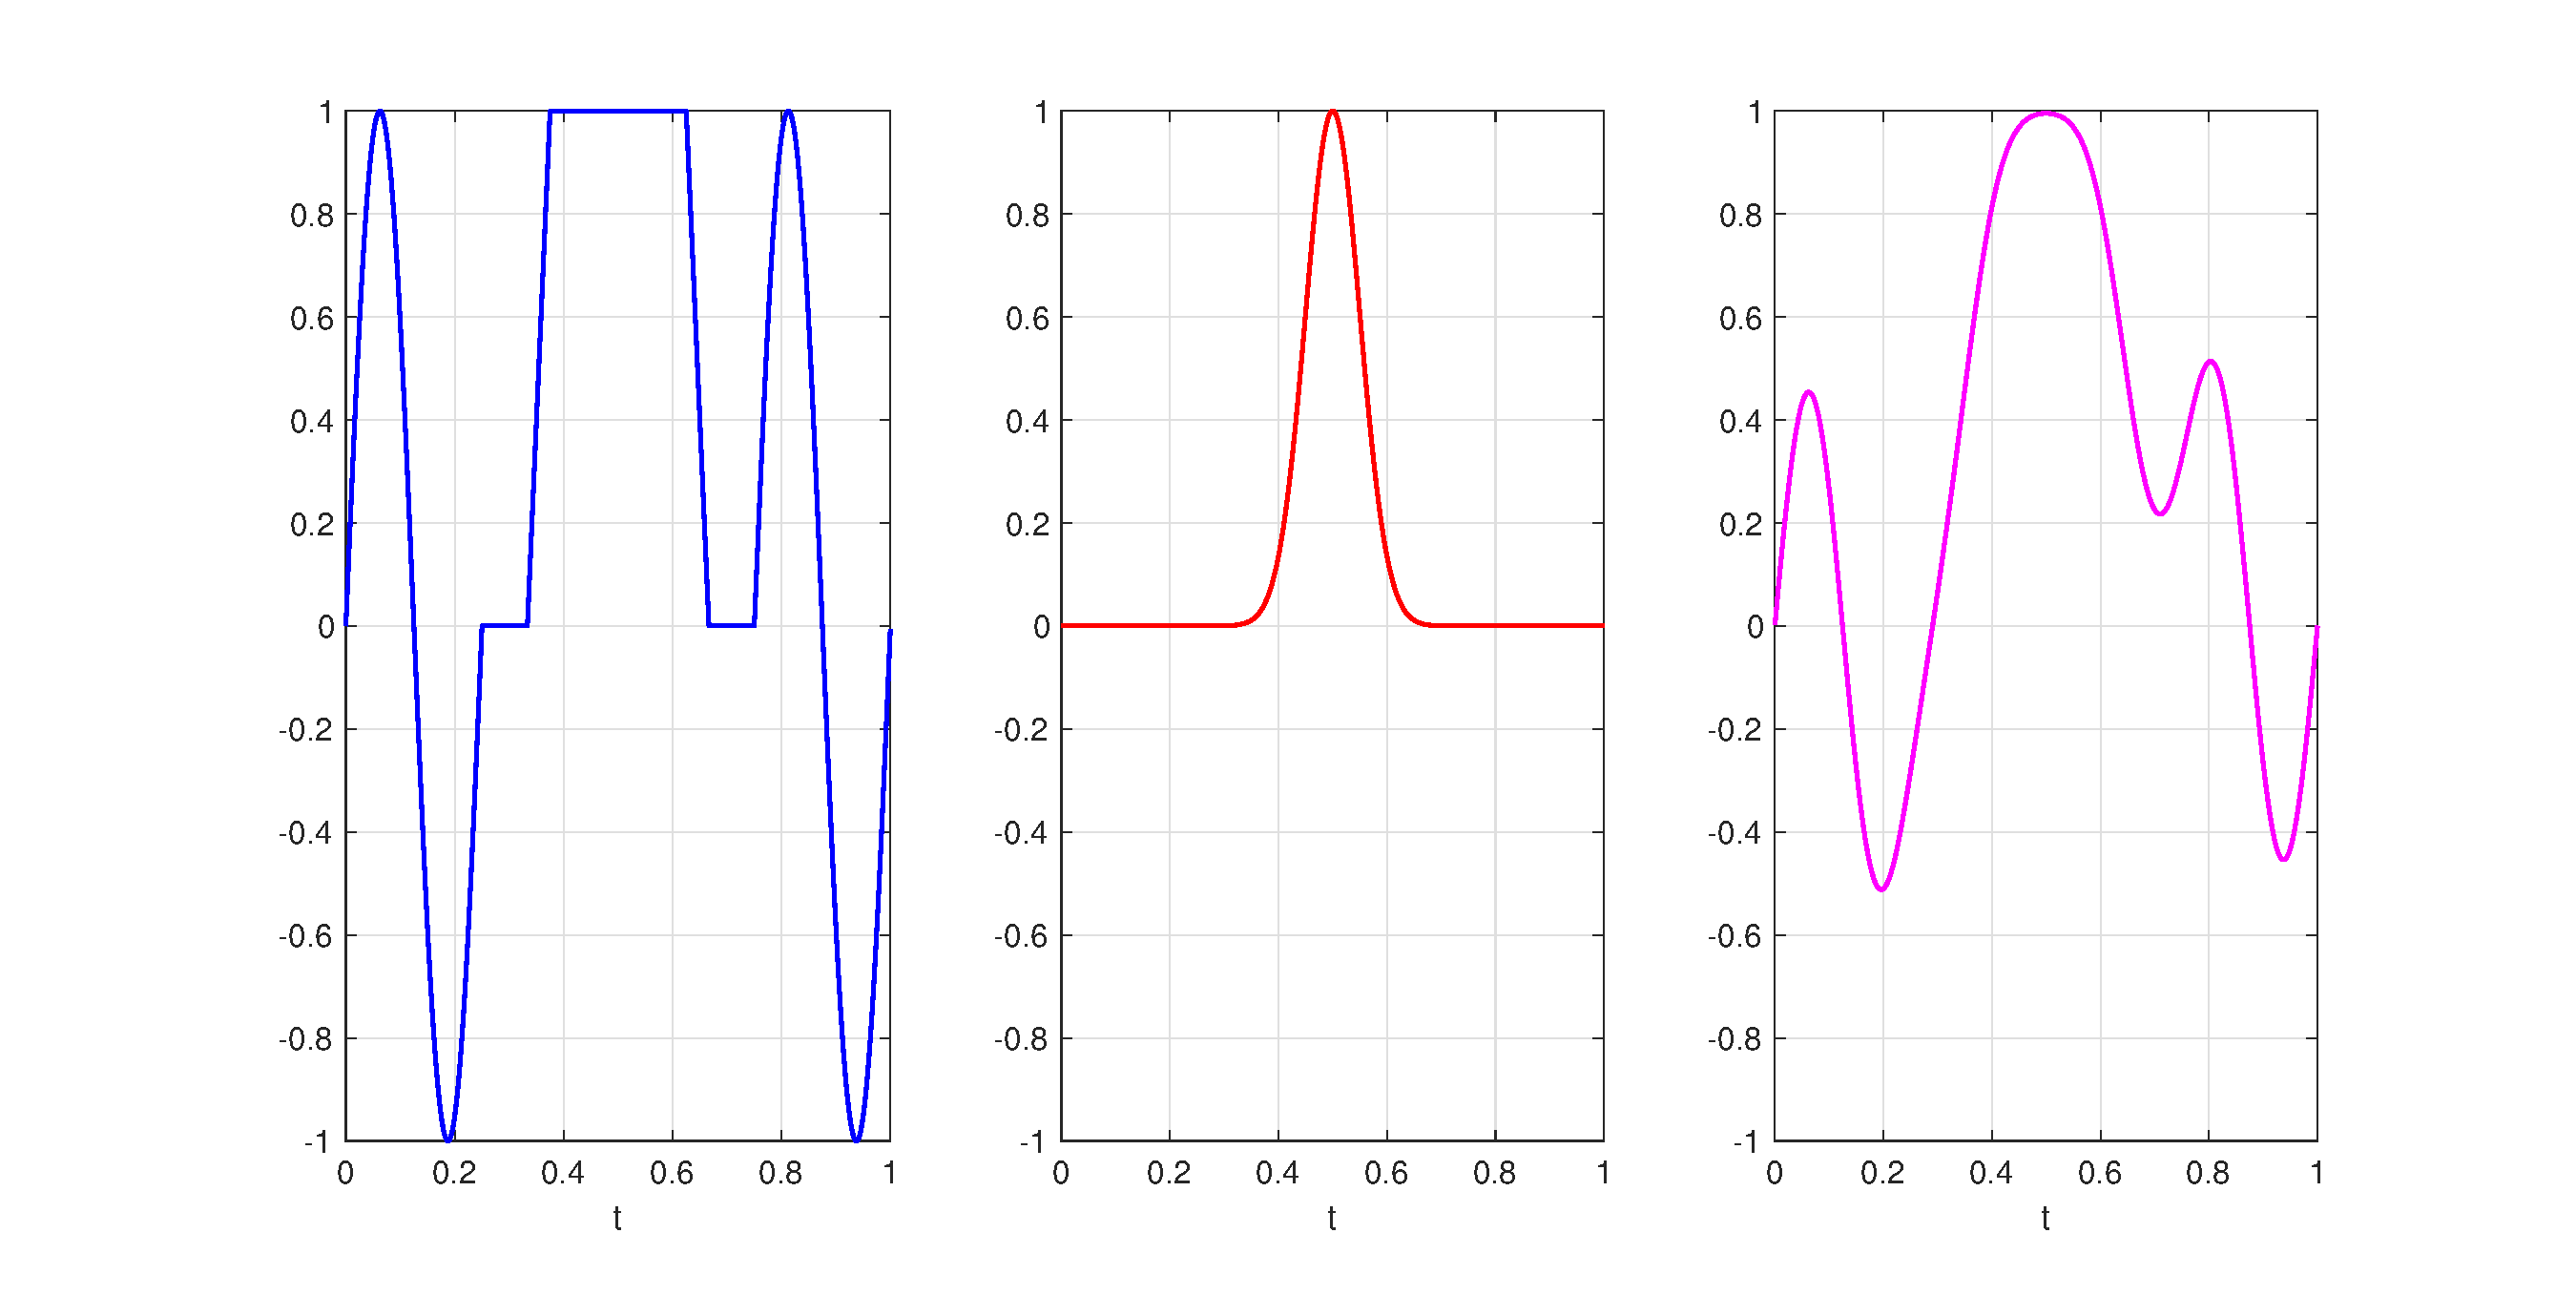
\includegraphics[scale=0.4]{Figures/FunctionKernelPlot.eps}}
\caption{Left: The graphs of the piecewise-smooth function $f(t)$. Right: The Gaussian kernel $k(t)$.}
\label{FunctionKernelPlot}
\end{figure}

\begin{figure}
	\centerline{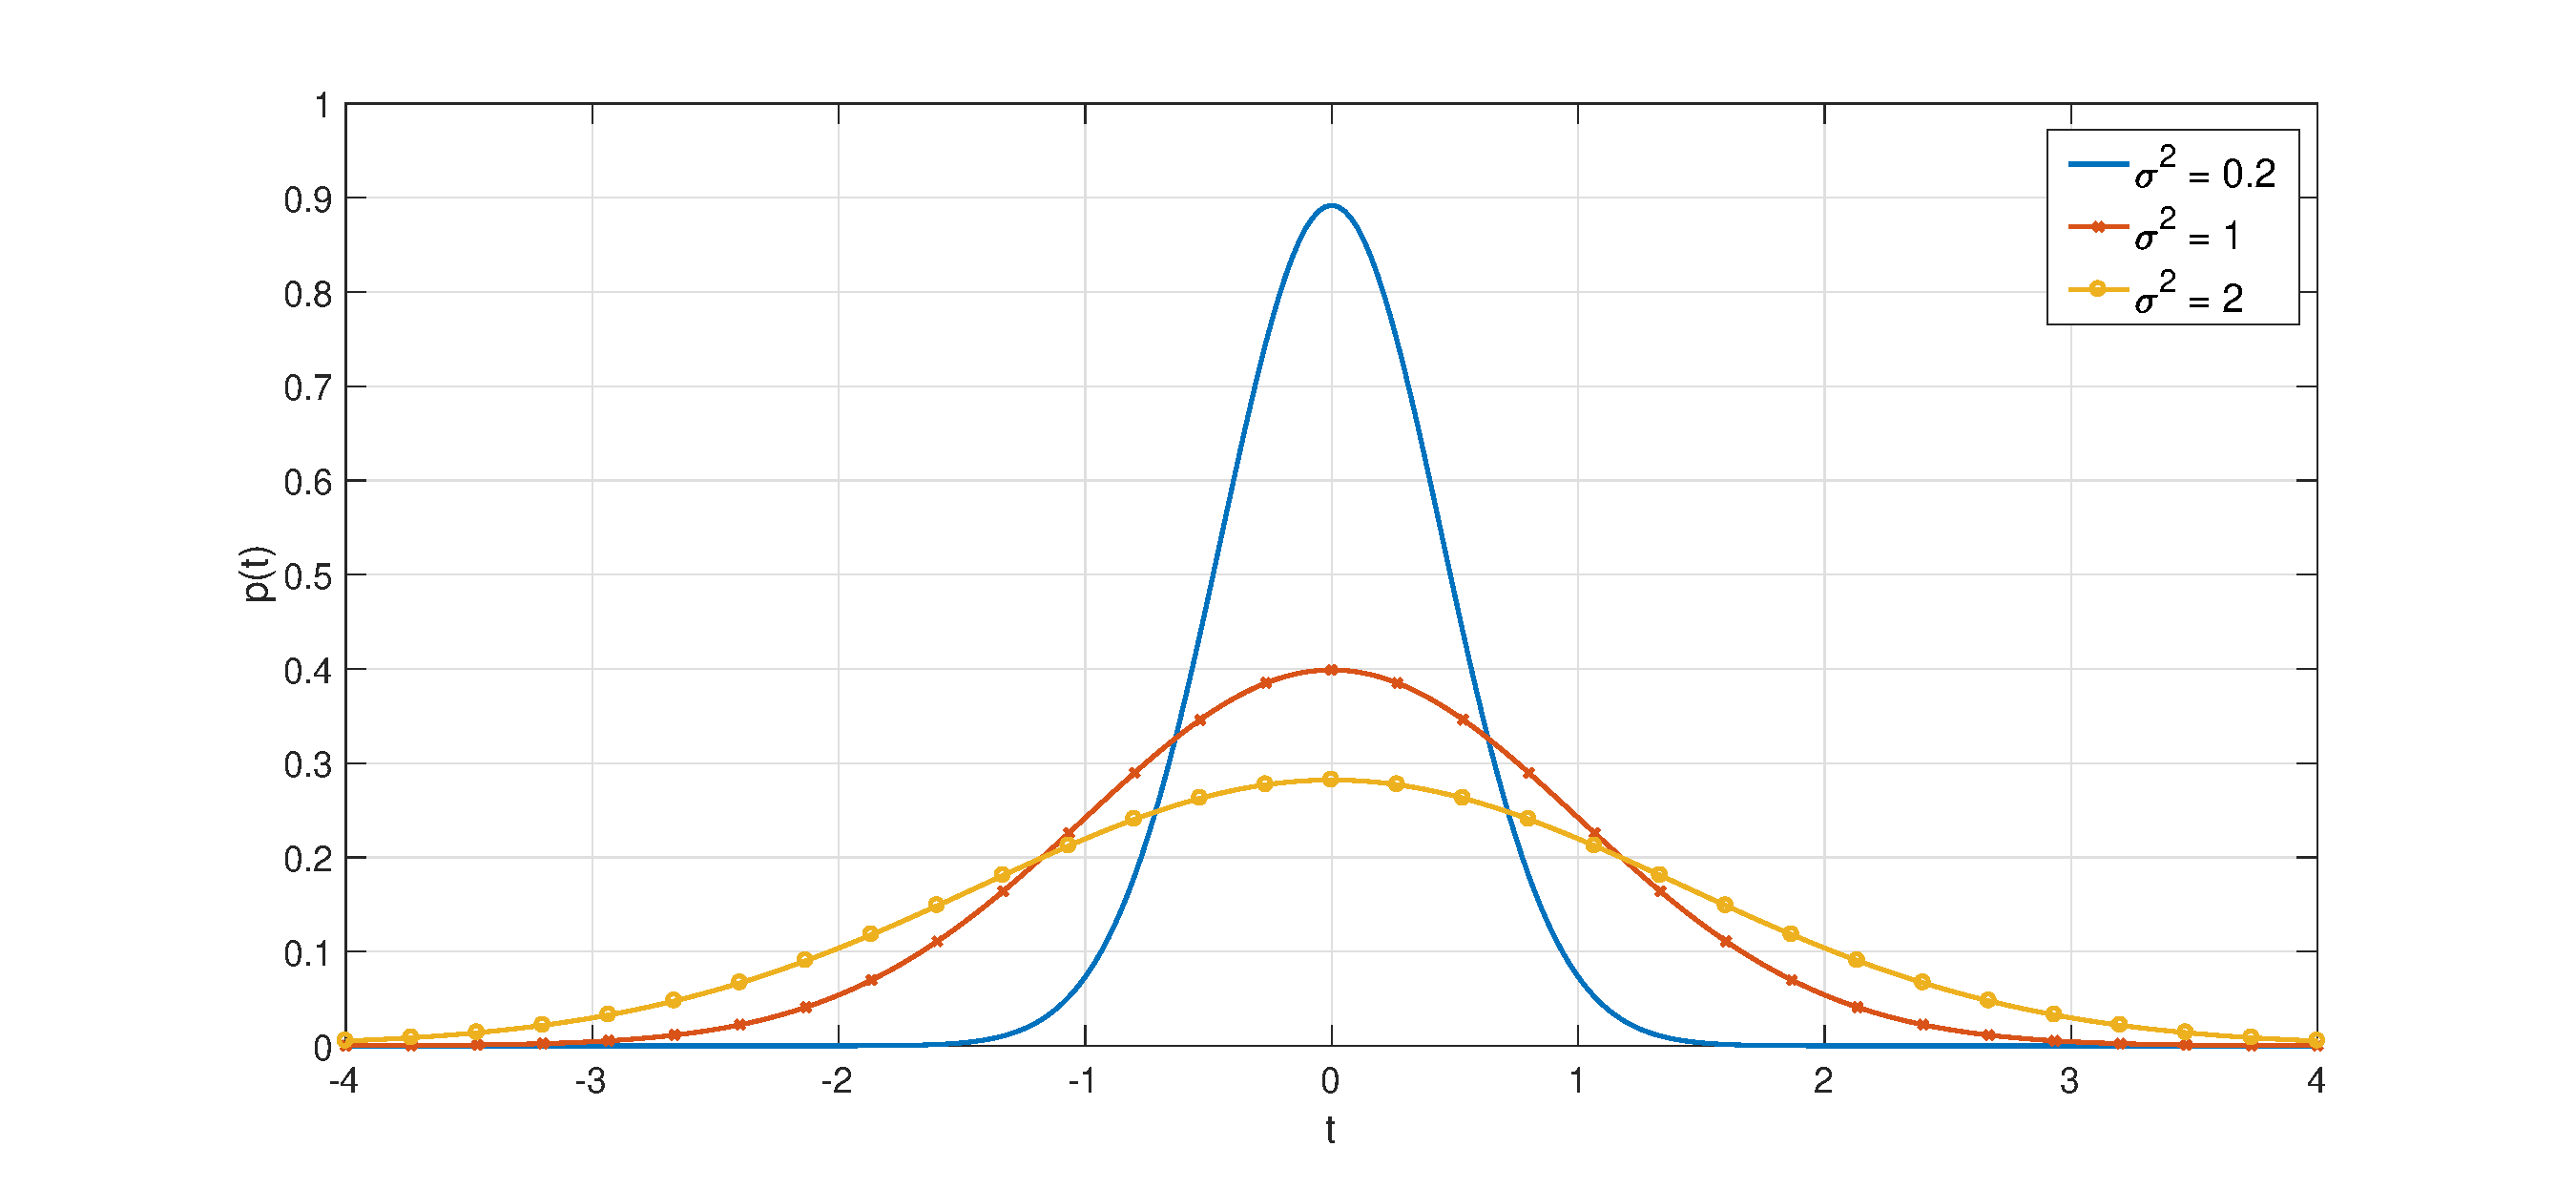
\includegraphics[scale=0.4]{Figures/GaussianDistributions.eps}}
\caption{Gaussian distributions for difference values of variance $\blurV$, all centered at the origin ($\mu = 0$). As $\blurV$ increases, the width of the distribution increases.}
\label{GaussianDistributions}
\end{figure}

To find a solution to the forward problem, which is the evaluation of $g = k * f$, a quadrature method can be used to find a numerical approximation to the convolution integral. In the discrete setting, (1) can be stated as
\begin{equation}
\gVec = \kMat\fVec,
\label{eq:Dis}
\end{equation}
where $\fVec$ and $\gVec$ are the vector discretization of $f$ and $g$, respectively, and $\kMat$ is a matrix representing the discrete convolution of $k$ with $f$. For example, suppose $k(x,t)$ is a zero-centered Gaussian kernel and the domain of integration in \eqref{eq:Con} is $[0,1]$. Given some $x_j \in [0,1]$, the continuous forward problem is to evaluate
\[g(x_j) = \int_0^1 \exp\left(\frac{-(x_j - t)^2}{2\blurV}\right)f(t) \: dt.\]
If a left Riemann sum is used with $t_k = (k-1)/n$ for $k \in \{1,2,\ldots,n\}$, representing an equispaced discretization of $[0,1]$ using $n$ points, then
\[g(x_j) \approx \sum_{k=1}^n \frac{1}{n}\exp\left(\frac{-(x_j - t_k)^2}{2\blurV}\right)f(t_j).\]
For approximations to $g(x)$ at the same points that make up the equispaced discretization of $[0,1]$, i.e. at the points $x_j = (j-1)/n$ for $j \in \{1,2,\ldots,n\}$, then \eqref{eq:Dis} is exactly the system that provides these approximations with $\fVec = [f(t_1),f(t_2),\ldots,f(t_n)]$, $\gVec = [g(x_1),g(x_2),\ldots,g(x_n)]$, and the elements of $\kMat$ being
\[K_{jk} = \frac{1}{n}\exp\left(\frac{-(j - k)^2}{2\blurV}\right).\]
Note that taking the collocation and quadrature points as the same ensures that the matrix $\kMat$ is square. Changing the number of collocation points, or the quadrature method, can change $\kMat$ from square to rectangular. \par
If the matrix $\kMat$ is nonsingular, then the solution to the inverse problem of \eqref{eq:Dis} is $\fVec = \kMat^{-1}\gVec$. As with many linear systems, however, direct matrix inversion is discouraged and usually impractical since the matrix $\kMat$ becomes increasingly ill-conditioned as the size of the system grows \cite{Vogel:2002}. Unfortunately, large systems are necessary to adequately approximate the continuous problem, and so other methods of solving for $\fVec$ must be considered. \par
Before discussing the consequences of ill-conditioning, the concept of an well-posed problem will be introduced, which is due to Hadamard. Given an operator $A : \mathcal{H}_1 \rightarrow \mathcal{H}_2$, where $\mathcal{H}_1$ and $\mathcal{H}_1$ are Hilbert spaces, the equation $Af = g$ is said to be well-posed if
\begin{enumerate}
\item[(i)] for each $g \in \mathcal{H}_2$ there exists a solution $f \in \mathcal{H}_1$ to $Af = g$,
\item[(ii)] the solution $f$ is unique, and
\item[(iii)] if $Af_* = g_*$ and $Af = g$, then $f \rightarrow f_*$ whenever $g \rightarrow g_*$.
\end{enumerate}
In order, these conditions require that a solution exists, is unique, and is stable under perturbations in $g$. If one of these conditions is not met, then $Af = g$ is said to be an ill-posed problem. The discrete version $\kMat\fVec = \gVec$ of the problem in this report is ill-posed: singularity of $\kMat$ violates conditions (i) and (ii), and a poor condition number of nonsingular $\kMat$ violates condition (iii). If the matrix $\kMat$ is rectangular, then $\kMat$ is singular and certainly (i) is violated.  \par 
A primary consequence of $\kMat$ being ill-conditioned relates to the accuracy of the vector $\gVec$. If $\gVec$ contains errors, as is often the case in practical applications, the errors are amplified during the multiplication $\kMat^{-1}\gVec$ since $\kMat$ is ill-conditioned and so the solution $\fVec$ will contain errors as well. In other words, $\fVec$ is sensitive to errors in $\gVec$. For this consideration, the following system will be the assumed model throughout this report
\begin{equation}
\gnoiseVec = \kMat\fVec + \noiseVec
\label{eq:DisNoise}
\end{equation}
where $\noiseVec$ is a vector that represents any errors in $\gVec$ (this is equivalent to the statement $\gnoiseVec = \gVec + \noiseVec$). For further simplicity, assume that $\noiseVec \sim \mathcal{N}(\bm{0},\noiseSD^2I)$, where $\bm{0}$ is the zero vector of length $n$ and $I$ is the $n \times n$ identity matrix. In other words, the error vector $\noiseVec$ is an $n$-dimension Gaussian random variable with mean zero and variance $\noiseSD^2$. 

\subsection{The Singular Value Decomposition} \label{sec:SVD}

Since direct matrix inversion is not practical, and at times not even possible since $\kMat$ can be singular, a singular value decomposition (SVD) of $\kMat$ can be an alternative. Assuming $\kMat$ is a real $m \times n$ matrix, the SVD of $\kMat$ is
\begin{equation}
\kMat = U\Sigma{V^\trans}
\label{eq:SVD}
\end{equation}
where the $m \times m$ matrix $U$ and the $n \times n$ matrix $V$ have orthogonal columns and $\Sigma$ is a $m \times n$ diagonal matrix. The diagonal elements of $\Sigma$ are the singular values of $\kMat$, denoted $\singular_i$ and satisfying $\singular_1 \geq \singular_2 \geq \ldots \geq \singular_n \geq 0$. The columns of $U$ and $V$ will be denoted $\LSV_i$ and $\RSV_i$, respectively; these vectors are known as the left and right singular vectors of $\kMat$, respectively. A matrix of complex values has a SVD as well, the only difference being that the transpose is replaced with conjugate transpose. \par
Let $r$ denote the rank of $\kMat$. Then $\singular_1 \geq \ldots \geq \singular_r > 0$, i.e. the number of nonzero singular values of $\kMat$ is equal to the rank of $\kMat$.  A common variation of the SVD is the compact SVD (or economy SVD \cite{golub2013matrix}), in which $\Sigma = \diag(\singular_1,\ldots,\singular_r)$, $U$ is an $m \times r$ matrix and $V^\trans$ is an $r \times n$ matrix. The matrices $U$ and $V$ are no longer orthogonal in the traditional sense because they are not square (unless $\kMat$ is nonsingular), though their columns remain orthonormal. For the remainder of this report all SVD's are assumed to be compact.  \par 
By using $\kMat^{-1} = V\Sigma^{-1}U^\trans$ when $\kMat$ is nonsingular, the product $\kMat^{-1}\gnoiseVec$ is
\begin{equation}
\kMat^{-1}\gnoiseVec = \kMat^{-1}\left(\kMat\fVec + \noiseVec\right) = \fVec + \kMat^{-1}\noiseVec = \fVec + V\Sigma^{-1}{U^\trans}\noiseVec = \fVec + \sum_{\ell = 1}^n \frac{{\LSV^\trans_\ell}\noiseVec}{\singular_\ell}\RSV_\ell. 
\label{eq:InvProd}
\end{equation}
Even if $\kMat$ is singular, a solution can still be obtained by using the psuedoinverse $\kMat^+ = V{\Sigma^+}U^\trans$, where $\Sigma^+ = \diag(1/\singular_1,\ldots,1/\singular_r)$, and the upper bound of summation in \eqref{eq:InvProd} becomes $r$. In either the nonsingular or singular case for $\kMat$, however, the summands in \eqref{eq:InvProd} are numerically unstable for small $\singular_i$. For a visual representation of this instability, a Picard plot can be constructed. A Picard plot is a graph showing the terms $|\LSV^\trans_i\noiseVec|/\singular_i$ in decreasing order with respect to the singular values. If the terms $|\LSV^\trans_i\noise|$ decay faster than $\singular_i$ as $i$ increases, then the terms $|\LSV^\trans_i\noiseVec|/\singular_i$ do not become excessively large; this is the discrete Picard condition \cite{ABT}. The discrete Picard condition is thus a measure of instability. If the discrete Picard condition is not met, then the terms $|\LSV^\trans_i\noiseVec|/\singular_i$ blow up as $i$ increases, often resulting in worthless solutions. In this experiment, the discrete Fourier transform will be used to obtain solutions analogous to those obtained by \eqref{eq:InvProd}. In Section \ref{sec:The Discrete Fourier Transform} a Picard plot is provided that demonstrates the relationship between the noise, the width of the Gaussian blur, and the resulting numerical instabilities related to obtaining meaningful solutions. See \cite{Hansen1990} for more information on Picard plots and the associated discrete Picard condition. \par 
A common approach to overcome numerical instabilities is to multiply the summands in \eqref{eq:InvProd} by \textit{filter functions} $\filt$ that depend upon $\singular_i$ and a non-negative \textit{regularization parameter} $\regparam$. By doing so, an approximate solution is obtained:
\begin{equation}
\fVec(\regparam) = \sum_{\ell = 1}^n \RSV_\ell\filt(\regparam,\singular_\ell)\left(\frac{{\LSV^\trans_\ell}\gnoiseVec}{\singular_\ell}\right) = V\Phi\Sigma^+U^\trans\gnoiseVec,
\label{eq:ApproxSol}
\end{equation}
where the matrix $\Phi$ is diagonal with $\Phi_{\ell\ell} = \filt(\regparam,\singular_\ell)$ for $\ell = 1,\ldots,n$. The most desired property of the filter functions is that $\filt(\singular_\ell)/\singular_\ell \approx 1$  for large values of $\singular_\ell$ and $\filt(\singular_\ell)/\singular_\ell \approx 0$ for small values of $\singular_\ell$.  Perhaps the simplest filter function is
\[\filt(\regparam,\singular_\ell) = \begin{cases}
1, & \singular_\ell^2 > \regparam \\
0, & \singular_\ell^2 \leq \regparam
\end{cases}\]
Using this function in (3) gives the approximate solution
\[\fVec(\regparam) = \sum_{\singular_\ell^2 > \regparam} \frac{{\LSV^\trans_\ell}\gnoiseVec}{\singular_\ell}\RSV_\ell\]
which actually corresponds to the solution obtained using a truncated singular value decomposition (TSVD) of the matrix $\kMat$ \cite{Vogel:2002}. \par

\subsection{Tikhonov regularization} \label{sec:Tikhonov reg.}

A less simple filter function is
\begin{equation}
\filt(\regparam,\singular_\ell)  = \frac{\singular_\ell^2}{\singular_\ell^2 + \regparam^2}
\label{eq:TikFilt}
\end{equation}
which is known as the Tikhonov filter function. For large values of $\regparam$, \eqref{eq:TikFilt} is close to zero and for small values of $\regparam$ (and nonzero values of $\singular_\ell$), it is close to one. Another property of \eqref{eq:TikFilt} is that for fixed nonzero $\singular_\ell$, it is monotone decreasing in $\regparam$. Tikhonov filter functions will be considered extensively through this report. Thus in addition, let
\begin{equation}
\mfilt(\regparam,\singular_\ell) = 1 - \filt(\regparam,\singular_\ell) = \frac{\regparam^2}{\singular_\ell^2 + \regparam^2}.
\label{eq:TikFiltPsi}
\end{equation}
The expression $1 - \filt(\regparam,\singular_\ell)$ arises a number of time in the methods introduced in Section \ref{sec:Parameter estimation methods}, and so $\mfilt(\regparam,\singular_\ell)$ will be used to simplify notation. In contrast to \eqref{eq:TikFilt}, \eqref{eq:TikFiltPsi} is close to one for large values of $\regparam$ and monotone increasing in $\regparam$ for fixed $\singular_\ell$; see Figure \ref{fig:Phi Psi Plot}. \par 

\begin{figure}
	\centerline{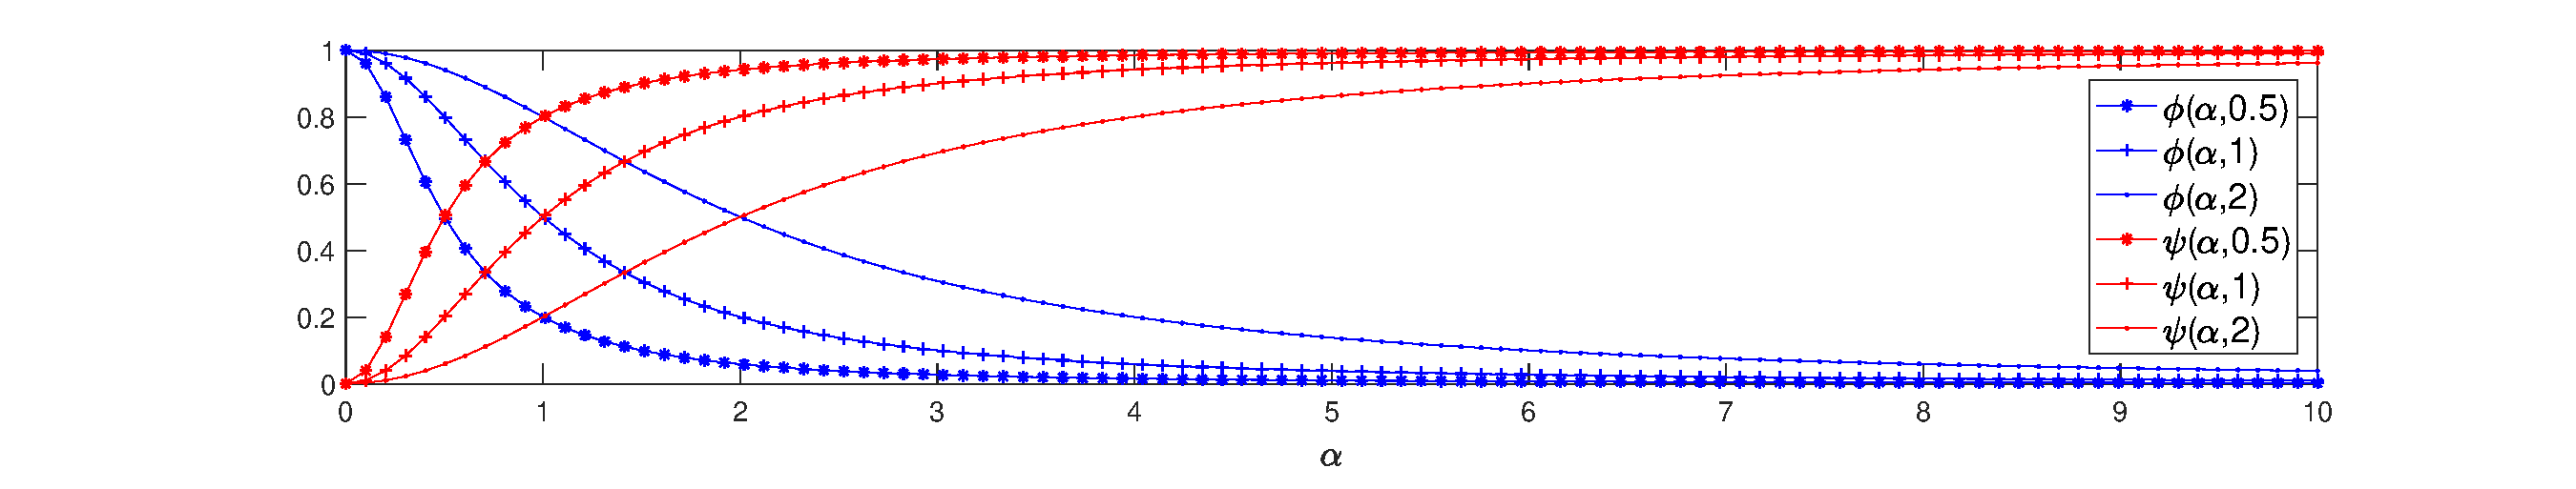
\includegraphics[scale = 0.5]{Figures/Phi_Psi_Plot.eps}}
\caption{The behavior of the Tikhonov filter function $\filt(\regparam,\singular_\ell)$ and corresponding $\mfilt(\regparam,\singular_\ell) = 1 - \filt(\regparam,\singular_\ell)$ is displayed for choice values of $\singular_\ell$. For fixed $\singular_\ell$, $\filt(\regparam,\singular_\ell) \rightarrow 0$ and $\mfilt(\regparam,\singular_\ell) \rightarrow 1$ as $\regparam \rightarrow \infty$. Notice also that $\filt(\regparam,\singular_\ell) = \mfilt(\regparam,\singular_\ell) = 1/2$ for $\alpha = \singular_\ell$.}
\label{fig:Phi Psi Plot}
\end{figure}

The use of the Tikhonov filter function to generate an approximate solution is known as \textit{Tikhonov regularization} \cite{Tikh1963}; in terms of an SVD, the obtained solution is
\begin{equation}
\fVec(\regparam) = \sum_{\ell = 1}^n \filt(\regparam,\singular_\ell)\frac{{\LSV^\trans_\ell}\gnoiseVec}{\singular_\ell}\RSV_\ell = \sum_{\ell = 1}^n \frac{\singular_\ell{\LSV^\trans_\ell}\gnoiseVec}{\singular_\ell^2 + \regparam^2}\RSV_\ell = V\Phi\Sigma^+U^\trans\gnoiseVec.
\label{eq:TikSol}
\end{equation}
An alternative (and more general) representation of the above Tikhonov solution is
\begin{equation}
\fVec(\regparam) = \arg\min_{\fVec \in \mathbb{R}^n} \|\kMat\fVec - \gnoiseVec\|^2 + \regparam^2\|D\fVec\|^2,
\label{eq:TikSol2}
\end{equation}
where $D$ is the matrix representation of a linear operator. The term $\|D\fVec\|^2$ is commonly called the penalty function \cite{Vogel:2002}. The representation \eqref{eq:TikSol} follows from selecting $D$ to be $I$, the $n \times n$ identity matrix. The solution \eqref{eq:TikSol2} can also be expressed in block form as
\begin{equation}
\fVec(\regparam) = \arg\min_{\fVec \in \mathbb{R}^n} \left\| \begin{bmatrix}
\kMat \\
\regparam D
\end{bmatrix}\fVec - \begin{bmatrix}
\gnoiseVec \\
\bm{0}
\end{bmatrix} \right\|^2.
\label{eq:TikSol3}
\end{equation}
If the matrix $D$ in \eqref{eq:TikSol2} is non-singular, then the substitutions $\mathbf{y} = D\fVec$, $A = \kMat{D}^{-1}$, and $\mathbf{b} = \gnoiseVec$ give
\begin{equation}
\mathbf{y}(\regparam) = \arg\min_{\mathbf{y} \in \mathbb{R}^n} \|A\mathbf{y} - \mathbf{b}\|^2 + \regparam^2\|\mathbf{y}\|^2.
\label{eq:TikSol Standard Form}
\end{equation}
This is known as standard form of the regularization problem. Once $\mathbf{y}$ is obtained from \eqref{eq:TikSol Standard Form}, the final solution is recovered by $\fVec = D^{-1}\mathbf{y}$.  \par 
However, there are many examples of matrices $D$ that are singular, such as finite difference matrices that approximate derivative operators. In such cases, the regularization can still be recast in standard form, which relies upon the introduction of the generalized singular value decomposition (GSVD). To simply the derivation of the GSVD, it will be assumed that the matrix $[\kMat, \regparam D]^\trans$ in \eqref{eq:TikSol3} has full column rank, which ensures that the solution $\fVec(\regparam)$ is unique. Another simplifying assumption being that the $p \times n$ matrix $D$ has full row rank. Under these assumptions \cite[p.~104]{ABT}, the matrices $\kMat$ and $D$ can be expressed as
\begin{equation}
\label{eq:GSVD matrices}
\kMat = U\Lambda X^\trans, \quad D = VMX^\trans
\end{equation}
where the matrices $U$, $V$, $\Lambda$, $M$, and $X$ satisfy the following: 
\begin{itemize}
\item $U$ is an orthogonal $m \times m$ matrix. 
\item $V$ is an orthogonal $p \times p$ matrix.
\item $\Lambda$ is an $m \times n$ matrix with the property that the nonzero entries satisfy
\[0 \leq \Lambda_{1,k+1} \leq \ldots \leq \Lambda_{m,k+m} \leq 1,\]
where $k = 0$ if $m > n$ and $k = n-m$ otherwise. 
\item $M$ is a diagonal $p \times n$ matrix with $M_{1,1} \geq \ldots \geq M_{p,p} \geq 0.$
\item $M^\trans M + \Lambda^\trans \Lambda = I$ (the dimension of the identity matrix being $n \times n$).
\item $X$ is a nonsingular $n \times n$ matrix.
\end{itemize}
The generalized singular values of $\kMat$ and $D$ are defined as $\gamma_\ell = \lambda_{\ell}/\mu_{\ell}$, where
\begin{equation}
\label{eq:GSVD lambda}
\lambda_\ell = \sqrt{(\Lambda^\trans \Lambda)_{\ell,\ell}}, \quad \mu_\ell = \sqrt{(M^\trans M)_{\ell,\ell}}
\end{equation}
for $\ell = 1,\ldots,n$. In contrast to the SVD, the generalized singular values are ordered $\gamma_1 \leq \ldots \leq \gamma_n$. It is also possible that $\mu_\ell = 0$ for some $\ell$, in which case $\gamma_\ell$ is not defined. Even when $\mu_\ell$ is small, the resulting value of $\gamma_\ell$ can be excessively large which again emphasizing the need for regularization. By applying the orthogonality properties of the GSVD matrices \cite[p.~105-106]{ABT}, the regularized solution \eqref{eq:TikSol3} can be expressed as
\begin{equation}
\label{eq:TikSol GSVD}
\fVec(\regparam) = \sum_{\ell=1}^n \frac{\gamma_\ell^2}{\gamma_\ell^2 + \regparam^2} \frac{U_{\cdot,\ell+k}^\trans\gnoiseVec}{\lambda_\ell}Y_{\cdot,\ell}.
\end{equation}
The terms $\gamma_\ell^2/(\gamma_\ell^2 + \regparam^2)$ are known as the GSVD filter factors, which are identical in form to the filter factors \eqref{eq:TikFilt}. \par 
With the derivation of the GSVD established, an extension the transformation that rendered \eqref{eq:TikSol Standard Form} is now stated \cite[p.~38]{Hansen:98}. First, a weighted version of the psuedoinverse $D^+$ is defined as
\[D_{\kMat}^+ = \left(I - \left(\kMat\left(I - D^+D\right)\right)^+\kMat\right)D^+\]
If $p \geq n$, then $D_{\kMat}^+$ is the same as $D^+$. We must also consider
\[\fVec_0 \equiv \left(\kMat\left(I - D^+D\right)\right)^+\gnoiseVec,\]
which is the component of the solution contained in $\nullspace(D)$.  Using the GSVD matrices from \eqref{eq:GSVD matrices}, $D_{\kMat}^+$ and $\fVec_0$ can be written as
\begin{equation}
\label{eq:Trans. 1}
D_{\kMat}^+ = X \begin{bmatrix}
M^{-1} \\
\mathbf{0}
\end{bmatrix}V^\trans, \quad \fVec_0 = \sum_{\ell=m+1}^{n} U_{\cdot,\ell}^\trans\gnoiseVec X_{\cdot,\ell}
\end{equation}
where $\bm{0}$ is the zero matrix of appropriate dimension. The form of the regularized solution can now be expressed as \eqref{eq:TikSol Standard Form} with substitutions $\mathbf{y} = D\fVec$, $A = \kMat{D_{\kMat}^+}$, and $\mathbf{b} = \gnoiseVec - \kMat\fVec_0$. This is shown by writing
\begin{align*}
\|A\mathbf{y} - \mathbf{b}\|^2 + \regparam^2\|\mathbf{y}\|^2 &= \|\kMat{D_{\kMat}^+}D\fVec - \gnoiseVec - \kMat\fVec_0\|^2 + \regparam^2\|D\fVec\|^2 \\
&=  \|\kMat({D_{\kMat}^+}D\fVec - \fVec_0) - \gnoiseVec\|^2 + \regparam^2\|D\fVec\|^2
\end{align*}
as well as 
\begin{align*}
{D_{\kMat}^+}D\fVec - \fVec_0 &= \left(I - \left(\kMat\left(I - D^+D\right)\right)^+\kMat\right)D^+D\fVec - \left(\kMat\left(I - D^+D\right)\right)^+\gnoiseVec \\
&= D^+D\fVec - \left(\kMat\left(I - D^+D\right)\right)^+\kMat D^+D\fVec - \left(\kMat\left(I - D^+D\right)\right)^+\gnoiseVec \\ 
&= D^+D\fVec - \left(\kMat\left(I - D^+D\right)\right)^+\left[\kMat D^+D\fVec + \gnoiseVec\right] \\
&= 
\end{align*}
The final solution is then recovered by $\fVec = D_{\kMat}^+\mathbf{y} + \fVec_0$. \newpage

\section{Analytical tools} \label{sec:Analytical tools}

A number of analytic tools are used in this experiment. First, convolutions and certain associated matrices will be discussed. The discrete Fourier transform and some properties will then be examined. Lastly, the effects and resulting statistics of the Fourier transform as applied to Gaussian noise will be presented.

\subsection{Discrete convolution} \label{sec:Discrete convolution}
As described in the Section \ref{sec:Introduction}, the operation of convolution arises in various settings pertaining to inverse problems. Discrete convolution will first be described  in a general setting, followed by specific instances and connections to the numerical experiments conducted in this report. \par
Let $(x_n)$ and $(y_n)$ be sequences of complex numbers indexed by the integers. Then the discrete convolution of $(x_n)$ and $(y_n)$, denoted $x*y$, is defined by
\[(x*y)_n = \sum_{\ell=-\infty}^\infty x_{n-\ell}y_\ell.\]
The series in the definition of discrete convolution is bi-infinite, meaning that the discrete convolution might not be well-defined for any two arbitrary sequences. For example, if $x_n = y_n = 1$ for all $n \in \mathbb{Z}$, then the series defining $(x*y)_n$ is $\sum_{j=-\infty}^\infty 1$, which does not converge. In various cases, however, the discrete convolution is well-defined. These cases include sequences having only finitely-many nonzero terms and sequences in $\ell^1$. (In fact, the set of sequences having finitely-many nonzero terms is a linear subspace of $\ell^1$).  \par 
Fortunately, real-world applications usually involve finite sequences (vectors), which can be thought of as infinite or bi-infinite sequences having finitely-many nonzero terms. While such sequences do not require the evaluation of infinite series to compute discrete convolutions, it is helpful to have general results regarding the length and indices of discrete convolutions. Let $(x_n)$ and $(y_n)$ be nonzero sequences with finitely-many nonzero terms. For $(x_n)$, the assumptions imply the existence of integers $s_x$ and $e_x$ such that $x_n = 0$ for all $n \in \mathbb{Z}$ with either $n < s_x$ or $e_x < n$. Such integers exist for $(y_n)$ and will be denoted $s_y$ and $e_y$. The choice of letters reflects the fact that $s$ and $e$ represent the starting and ending indices of the section of the sequence where the terms can be nonzero. Extending this notation, the number of terms in this section of sequence is $n_x = e_x - s_x + 1$ and $n_y = e_y - s_y + 1$ for $(x_n)$ and $(y_n)$, respectively. From \cite{BoggessAlbert2001Afci}, the values of $s_{x*y}$, $e_{x*y}$, and $n_{x*y}$ are
\begin{align}
s_{x*y} &= s_x + s_y, \nonumber \\
e_{x*y} &= e_x + e_y, \label{eq:ConResults} \\
n_{x*y} &= n_x + n_y - 1. \nonumber
\end{align}
As an illustrative example, let $\mathbf{x} = [1,2,3]$ and $\mathbf{y} = [4,5,6,7]$ be row vectors. The vectors can be thought of as the bi-infinite sequences $(x_n) = (\ldots,0,1,2,3,0\ldots)$ and $(y_n) = (\ldots,0,4,5,6,7,0,\ldots)$. If the sequences are indexed so that $x_1 = 1$ and $y_1 = 4$, then $s_x = s_y = 1$, $e_x = n_x = 3$, and $e_y = n_y = 4$. Then by \eqref{eq:ConResults}, $s_{x*y} = 2$, $e_{x*y} = 8$, and $n_{x*y} = 6$. The bi-infinite sequence produced from the convolution is
\[x*y = (\ldots,0,4,13,28,34,32,21,0,\ldots),\]
where $(x*y)_2 = 4$ and $(x*y)_8 = 21$. \par 
Since the numerical experiments for this report are conducted in MATLAB, a brief remark regarding discrete convolutions in MATLAB is be given. If the built-in function \texttt{conv} is used to evaluate the discrete convolution of row vectors $\mathbf{x}$ and $\mathbf{y}$ described in the previous example, the output is the row vector $[4,13,28,34,32,21]$.  All vectors in MATLAB have a starting index of 1, and the vector resulting from the convolution is no different: the component 4 has an index of 1. While this seems to conflict with \eqref{eq:ConResults} (recall that $s_{x*y} = 2$, not 1), from a practical standpoint there is little reason for concern; usually the components themselves are of interest and not the indexing of the bi-infinite sequence. If one wants to keep track of the indexing as the convolution is evaluated, index vectors can be defined for $\mathbf{x}$ and $\mathbf{y}$ and \eqref{eq:ConResults} can be applied to obtain an index vector for the resulting convolution. See \cite{BoggessAlbert2001Afci} for an explicit MATLAB example. \par 

\subsection{Circulant matrices} \label{sec:Circulant matrices}
In Section \ref{sec:Discrete convolution}, the discrete convolution and some of its variants were discussed. In this section, matrices will be discussed that have connections to discrete convolutions and other concepts. \par 
The first type of matrix to be discussed is a \textit{Toeplitz matrix}. A matrix $T$ is called a Toeplitz matrix if it is constant along each diagonal. The following matrices are examples of Toeplitz matrices.
\[A = \begin{bmatrix}
1 & 2 \\
2 & 1 \\
3 & 2
\end{bmatrix}, \quad 
B = \begin{bmatrix}
1 & 2 & 3 \\
2 & 1 & 2 
\end{bmatrix}, \quad 
C = \begin{bmatrix}
1 &  2 \\
2 & 1
\end{bmatrix}.\]
It is important to notice that by definition, Toeplitz matices need not be square. \par 
The primary connection to be made in this report is that discrete convolutions can be described in the context of matrix-vector multiplication using Toeplitz matrices. For example, the discrete convolution of $\mathbf{x} = [1,2,3]$ and $\mathbf{y} = [4,5,6,7]$ from Section \ref{sec:Discrete convolution} can be cast as a matrix-vector product by defining a matrix $X$ to be
\[X = \begin{bmatrix}
1 & 0 & 0 & 0 \\
2 & 1 & 0 & 0 \\
3 & 2 & 1 & 0 \\
0 & 3 & 2 & 1 \\
0 & 0 & 3 & 2 \\
0 & 0 & 0 & 3
\end{bmatrix}.\]
Certainly $X$ is a Toeplitz matrix, and $x*y$ can be expressed as $Xy^\trans$ with $x*y$ being a (column) vector of length $n_{x*y} = 6$; the length of this vector agrees with result \eqref{eq:ConResults}. The operation $Xy^\trans$ is equivalent to \texttt{conv(x,y)} in MATLAB. \par 
If a matrix $C$ has the property that each row is the circular right shift of the components of the preceding row, then $C$ is called a \textit{circulant matrix}. The \textit{circular right shift} of a row vector $[x_1,x_2,\ldots,x_n]$ is $[x_n,x_1,\ldots,x_{n-1}]$. From this definition, every circulant matrix is also a Toeplitz matrix. Just like Toeplitz matrices, circulant matrices need not be square. For example,
\[C = \begin{bmatrix}
1 & 2 & 3 & 4 \\
4 & 1 & 2 & 3 \\
3 & 4 & 1 & 2
\end{bmatrix}\] 
is a circulant matrix generated by circular right shifts of the vector $[1,2,3,4]$. However, circulant matrices are often defined to be square, a convention that will be adopted in this report. Therefore every reference to circulant matrices from this point will be under the assumption that circulant matrices are square. A significant property of circulant matrices is that they are diagonalized by the discrete Fourier transform, a property that will be discussed in Section \ref{sec:The Discrete Fourier Transform}.

\subsection{The Discrete Fourier Transform} \label{sec:The Discrete Fourier Transform}
The discrete Fourier transform will be introduced from the perspective of approximating coefficients of the Fourier series of a $2\pi$-periodic function $f$. On the interval $[0,2\pi]$, the $k$th complex Fourier coefficient of $f$ is given by
\[c_k = \frac{1}{2\pi}\int_0^{2\pi} f(t)\exp(-ikt)\:dt,\]
where $i = \sqrt{-1}$.  Applying the trapezoidal rule for approximating this integral with $n$ points then produces
\[c_k \approx \frac{1}{n}\sum_{j = 0}^{n-1} f\left(\frac{2\pi{j}}{n}\right)\exp\left(\frac{-2\pi{ijk}}{n}\right).\]
This approximation is accurate for $k$ significantly smaller than the number of points $n$. \par 
The \textit{discrete Fourier transform} (DFT) is a mapping $\mathcal{F}:\mathbb{C}^n \rightarrow \mathbb{C}^n$ defined by
\begin{equation}
\mathcal{F}(\mathbf{f})_k = \frac{1}{\sqrt{n}}\sum_{j=0}^{n-1} f_{j}\exp\left(\frac{-2\pi{ijk}}{n}\right), \quad \mathbf{f}\in\mathbb{C}^n, \quad 0 \leq k \leq n-1.
\label{eq:DFT}
\end{equation}
The DFT of a vector $\mathbf{f}$ will be denoted by $\widehat{\mathbf{f}}$. The inverse DFT of a vector $\widehat{\mathbf{f}}$ is given by
\begin{equation}
\mathcal{F}^{-1}(\widehat{\mathbf{f}})_k = \frac{1}{\sqrt{n}}\sum_{j=0}^{n-1} \widehat{f}_j\exp\left(\frac{2\pi{ijk}}{n}\right) = \mathbf{f}
\end{equation}
These definitions are nonstandard; typically the factors $1/\sqrt{n}$ in both the forward and inverse DFT definitions are combined as a single factor of $1/n$ in the definition of the forward DFT. The DFT can also be stated in terms of matrix-vector multiplication. Given an $\mathbf{f} \in \mathbb{C}^n$, $\widehat{\mathbf{f}}$ can be expressed as $F\mathbf{f}$ where the matrix $F\in\mathbb{C}^{n\times{n}}$ has components
\begin{equation}
F_{jk} = \frac{1}{\sqrt{n}}\exp\left(\frac{-2\pi{ijk}}{n}\right), \quad 0 \leq j,k \leq n-1.
\label{eq:DFT-Matrix}
\end{equation}
The matrix representing the inverse DFT is then $F^\ctrans$, where $\ctrans$ denotes conjugate transposition. A property of $F$ is that $F^\ctrans F = FF^\ctrans = (1/n)\diag(n) = I$, and so splitting the factor of $1/n$ as $(1/\sqrt{n})(1/\sqrt{n})$ for the definition of the DFT provides the benefit of $F$ being a unitary matrix. \par 
As stated previously, a significant property of circulant matrices is that they are diagonalized by the DFT. Using the definition of the $n \times n$ unitary Fourier matrix $F$, the property can be stated as
\begin{equation}
C = F^\ctrans\diag(\widehat{\mathbf{c}})F,
\label{eq:CircDiag}
\end{equation}
where $C$ is any $n \times n$ circulant matrix and $\widehat{\mathbf{c}}$ is the DFT of the first row of $C$ (recall that the rows of a circulant matrix are circulant right shifts a single row vector of length $n$). The components of $\widehat{\mathbf{c}}$ and the columns of $F^\ctrans$ are the eigenvalues and eigenvectors, respectively, of $C$. For a proof of this property, see \cite{BoggessAlbert2001Afci} or \cite{Vogel:2002}. \par
Now the properties of the DFT will be connected with the SVD of a circulant matrix, which will be the basis for the experiment design in Section \ref{sec:Experiment design}. Let $\fVec$ and $\kVec$ be the $N$-point discretizations of functions $f$ and $k$ on some interval $[a,b]$. Then the cyclic convolution $\gVec = \kVec * \fVec$ can be computed as a matrix-vector product by constructing an $N \times N$ circulant matrix $\kMat$ from $\kVec$. This construction is carried out by setting the first row of $\kMat$ to be $\kVec$, and each subsequent row to be a circular right shift of the preceding row (see \ref{sec:Circulant matrices}). In MATLAB, the command \texttt{toeplitz([k(1) fliplr(k(2:end))], k)} constructs the matrix $\kMat$. Then $\gVec = \kMat\fVec$, and after the addition of noise the equation \eqref{eq:DisNoise} is obtained. Then by using the property \eqref{eq:CircDiag} with the $N \times N$ unitary Fourier matrix $F$ and assuming that $\kMat$ is invertible, 
\begin{equation}
\kMat^{-1}\gnoiseVec = \fVec + (F^*\diag(\widehat{\kVec})F)^{-1}\noiseVec = \fVec + F^*\diag(\widehat{\kVec})^{-1}F\noiseVec = \fVec + \sum_{\ell = 0}^{n-1} [F^*]_\ell\left(\frac{\widehat{\noise}_\ell}{\widehat{k}_\ell}\right),
\label{eq:InvProdDFT}
\end{equation}
where $\widehat{\noise}_i$ and $\widehat{k}_i$ are the $i$th Fourier coefficients of $\noiseVec$ and $\kVec$, respectively, and $[F^*]_i$ is the $i$th column of the matrix $F^*$. Analogous to \eqref{eq:InvProd}, instabilities can arise if $\widehat{k}_i$ is small. By introducing filter factors to reduce possible instability, an approximate solution
\begin{equation}
\fVec(\regparam) = \sum_{\ell = 0}^{n-1} [F^*]_\ell\left(\frac{\filt(\regparam,\widehat{k}_\ell)\widehat{\gnoise}_\ell}{\widehat{k}_\ell}\right) = F^\ctrans\Phi\widehat{\kMat}^+F\gnoiseVec
\label{eq:ApproxSolDFT}
\end{equation}
can be obtained analogous to \eqref{eq:ApproxSol}, where $\widehat{\kMat}^+ = \diag(1/\widehat{\kVec})$.
Since $F^*$ is a matrix representation of the inverse DFT, the approximate solution can be rewritten as
\[\fVec(\regparam) = F^* \frac{\filt(\regparam,\widehat{\kVec})\widehat{\gnoiseVec}}{\widehat{\kVec}}.\]
Here $\filt(\regparam,\widehat{\kVec})\widehat{\gnoiseVec}/{\widehat{\kVec}}$ is a vector where the operations of multiplication and division are performed component-wise. This representation is useful for making a connection with the MATLAB implementation. \par
As mentioned in Section \ref{sec:Introduction}, a Picard plot is often useful in analyzing the numerical instabilities of solutions obtained from either or \eqref{eq:InvProd} or \eqref{eq:InvProdDFT}. Figure \ref{PicardPlot} shows an example of a Picard plot. The terms $|\widehat{k}_i|$ decrease down to machine precision, though the $|\widehat{\gnoise}_i|$ decrease but then level off just above the variance in the noise. As a result, the terms $|\widehat{\gnoise}_i|/|\widehat{k}_i|$ only decrease so far and then begin increasing. The steady increase can produce a blow up of the approximate solution. While illustrating these relationships, a Picard plot is also useful in determining how to truncate the sum in \eqref{eq:ApproxSolDFT} to avoid blow up in the solution. For the plot in Figure \ref{PicardPlot}, the sum in \eqref{eq:ApproxSolDFT} should be truncated around index 8 to obtain a meaningful solution. \par 

\begin{figure}[htb]
	\centerline{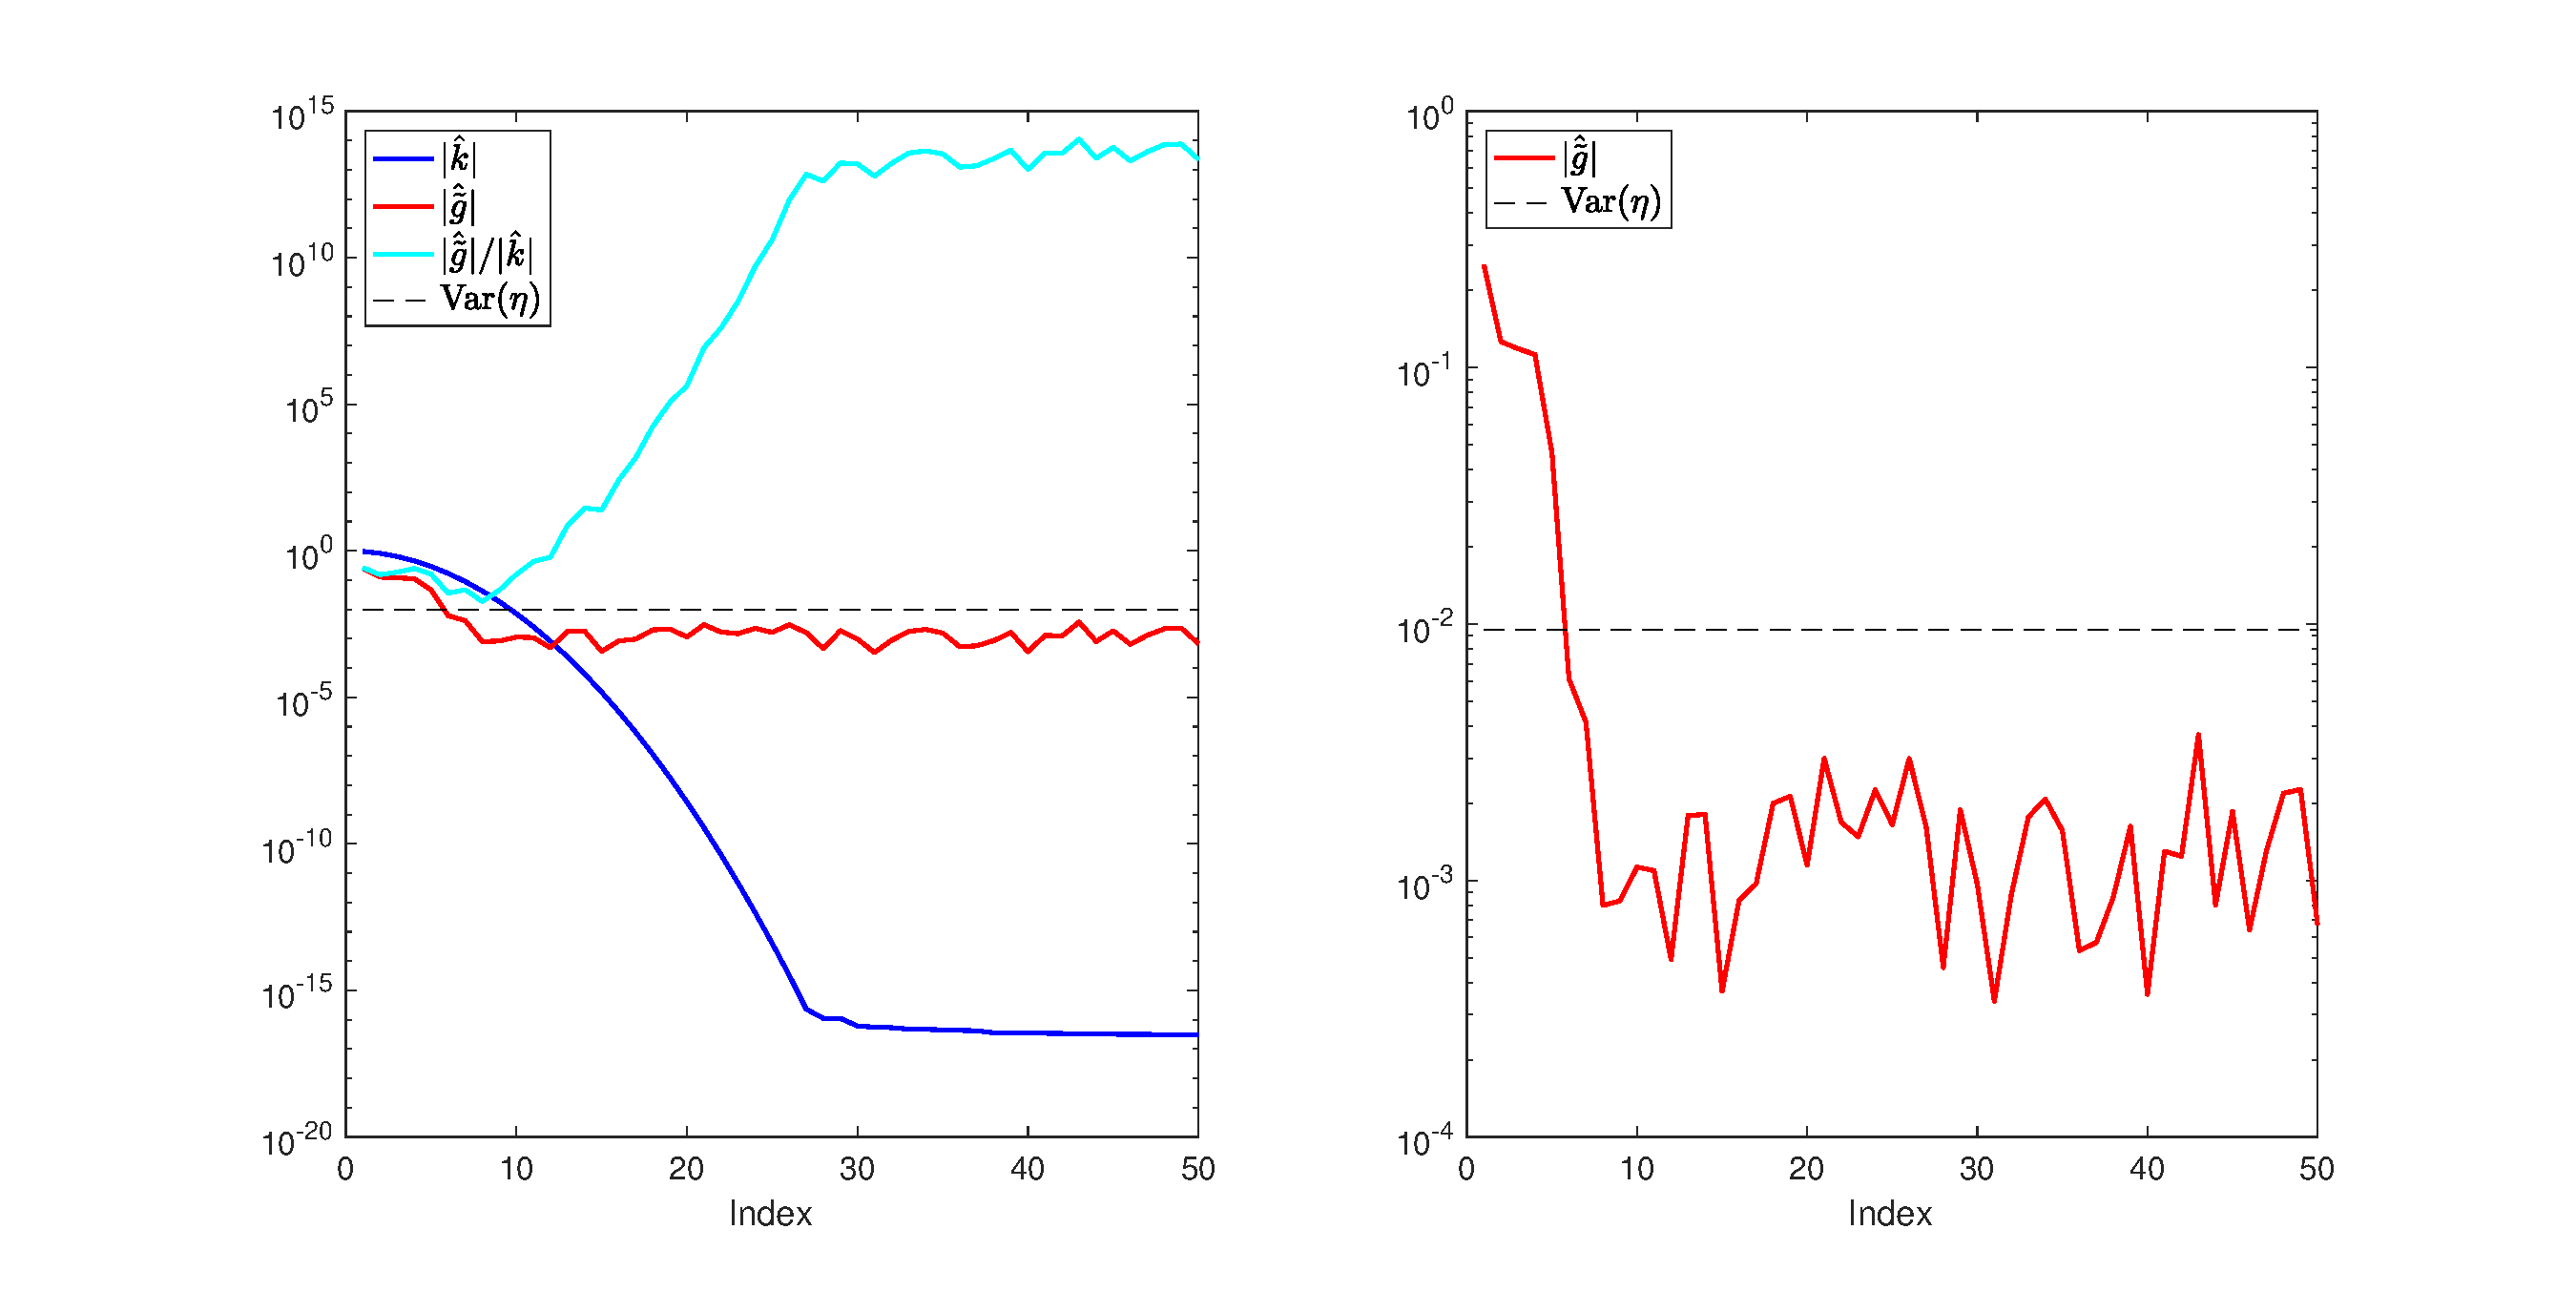
\includegraphics[scale = 0.45]{Figures/PicardPlot1D_F2_S15_W200.eps}}
\caption{(Left) A Picard plot generated from the second test function, a Gaussian blur with a width of 200, and an SNR of 15. The terms $|\widehat{\gnoise}_i|/|\widehat{k}_i|$ decrease until index 8, at which case the terms increase in magnitude. This is due to the fact that the $|\widehat{k}_i|$ steadily decrease, while the $|\widehat{\gnoise}_i|$ level off just below the variance in the noise. (Right) A zoom-in of the Picard plot is provided, showing that elements of the DFT of $\gnoiseVec$ decay only slightly below the variance of the noise in $\gnoiseVec$.}
\label{PicardPlot}
\end{figure}

While the connection between lines \eqref{eq:InvProdDFT} and \eqref{eq:ApproxSolDFT} and the SVD have been noted in regard to the structure of the terms and equations, a complete connection can be made if another property about $\kMat$ is assumed. Until this point $\kMat$ is assumed to be an invertible $N \times N$ circulant matrix formed from a vector $\kVec$. If $\kMat$ is also assumed to be symmetric, then the SVD of $\kMat$ is the same as the diagonalization by the unitary DFT matrix $F$ and the singular values of $\kMat$ are also the eigenvalues. \newpage

\section{Statistical considerations} \label{sec:Stats.}

Since the parameter estimation methods in Section \ref{sec:Parameter estimation methods} involve DFT's of the vector $\gnoiseVec = \gVec + \noiseVec$, some results regarding the distribution of the components of $\widehat{\noiseVec}$ will be presented. The first results will be in regard to the real and imaginary parts of the $\widehat{\noiseVec}$. Letting $A$ and $B$ be the real and imaginary parts, respectively, of the $n \times n$ DFT matrix, Euler's identity gives
\begin{equation}
A_{jk} = \frac{1}{\sqrt{n}}\cos\left(\frac{-2\pi{jk}}{n}\right), \quad B_{jk} = \frac{1}{\sqrt{n}}\sin\left(\frac{-2\pi{jk}}{n}\right),
\label{eq:Components Re(F) and Im(F)}
\end{equation}
for $0 \leq j,k \leq n-1$. It is clear from \eqref{eq:Components Re(F) and Im(F)} that the matrices $A$ and $B$ are symmetric. The rows (and by symmetry, columns) of $A$ and $B$ have the following orthogonality properties.
\begin{lemma}
\label{lem:Inner products}
Let $A$ and $B$ be the real and imaginary parts, respectively, of the $n \times n$ DFT matrix, and let $\langle\cdot,\cdot\rangle$ denote standard inner product (dot product) of $\mathbb{R}^n$. Then for $0 \leq j,k \leq n-1$:
\begin{enumerate}[label=(\roman*)]
\item $\langle A_{j,\cdot}, B_{k,\cdot}\rangle = 0$.
\item If $n$ is even, then 
\begin{align*}
\langle A_{j,\cdot}, A_{k,\cdot}\rangle &= \begin{cases}
1 & j = k = 0 \text{ or } j = k = n/2 \\ 
1/2 & j = k \neq 0 \text{ or } j = k \neq n/2 \\ 
1/2 & j \neq k \text{ and } k = n - j \\ 
0 & \text{otherwise} \end{cases}, \\
\langle B_{j,\cdot}, B_{k,\cdot}\rangle &= \begin{cases}
0 & j = k = 0 \text{ or } j = k = n/2 \\ 
1/2 & j = k \neq 0 \text{ or } j = k \neq n/2 \\ 
-1/2 &  j \neq k \text{ and } k = n - j \\ 
0 & \text{otherwise} \end{cases}.
\end{align*}
Equivalently,
\[AA^\trans = \frac{1}{2}I + \frac{1}{2}\left(\bm{e}_0^{}\bm{e}_0^\trans + \bm{e}_{n/2}^{}\bm{e}_{n/2}^\trans + \tilde{I}\right), \quad BB^\trans = \frac{1}{2}I - \frac{1}{2}\left(\bm{e}_0^{}\bm{e}_0^\trans + \bm{e}_{n/2}^{}\bm{e}_{n/2}^\trans + \tilde{I}\right),\]
where $\tilde{I}$ denotes the exchange matrix.
\item If $n$ is odd, then
\[\langle A_{j,\cdot}, A_{k,\cdot}\rangle = \begin{cases}
1 & j = k = 0 \\ 
1/2 & j = k \neq 0 \\
1/2 & j+k = n \\
0 & \text{otherwise} \end{cases}, \quad 
\langle B_{j,\cdot}, B_{k,\cdot}\rangle = \begin{cases}
0 & j = k = 0 \\ 
1/2 & j = k \neq 0 \\
-1/2 & j+k = n \\
0 & \text{otherwise} \end{cases}.\]
Equivalently,
\[AA^\trans = \frac{1}{2}I + \frac{1}{2}\left(\bm{e}_0^{}\bm{e}_0^\trans + \tilde{I}\right), \quad BB^\trans = \frac{1}{2}I - \frac{1}{2}\left(\bm{e}_0^{}\bm{e}_0^\trans + \tilde{I}\right).\]
\end{enumerate}
Notice that in both the even and odd cases, $AA^\trans + BB^\trans = I$.
\end{lemma}
\begin{proof}
Property (i) will first be established. Letting $A$ and $B$ be as required, \eqref{eq:Components Re(F) and Im(F)} gives
\begin{equation}
\langle A_{j,\cdot}, B_{k,\cdot}\rangle = \frac{1}{n}\sum_{\ell=0}^{n-1}\cos\left(\frac{-2\pi{j\ell}}{n}\right)\sin\left(\frac{-2\pi{\ell{k}}}{n}\right) = \frac{1}{n}\sum_{\ell=0}^{n-1}\cos\left(-\theta_{j\ell}\right)\sin\left(-\theta_{k\ell}\right),
\label{eq: <Re(F),Im(F)>}
\end{equation}
where $\theta_{j\ell} = 2\pi{j\ell}/n$. Applying the appropriate product-to-sum trigonometric identity and using the fact that sine is an odd function allows for sum in \eqref{eq: <Re(F),Im(F)>} to be evaluated as
\begin{align*}
\frac{1}{n}\sum_{\ell=0}^{n-1}\cos\left(-\theta_{j\ell}\right)\sin\left(-\theta_{k\ell}\right) &= \frac{1}{2n}\sum_{\ell=0}^{n-1}\left[\sin\left(-\theta_{(j+k)\ell}\right) - \sin\left(-\theta_{(k-j)\ell}\right)\right] \\
&= \frac{1}{2n}\sum_{\ell=0}^{n-1}\left[\sin\left(\theta_{(k-j)\ell}\right) - \sin\left(\theta_{(j+k)\ell}\right)\right] \\
&= \frac{1}{2n}\left(s_1 - s_2\right),
\end{align*}
where
\[s_1 = \sum_{\ell=0}^{n-1}\sin\left(\theta_{(k-j)\ell}\right), \quad s_2 = \sum_{\ell=0}^{n-1}\sin\left(\theta_{(j+k)\ell}\right).\]
Both $s_1$ and $s_2$ are of the form $\sum_{\ell=0}^{n-1} \sin(\theta_{p\ell})$, where $p$ is an integer (either $k-j$ or $j+k$). This form can be written as
\[\sum_{\ell=0}^{n-1} \sin\left(\theta_{p\ell}\right) = \Im\left(\sum_{\ell=0}^{n-1} \exp\left(i\theta_{p\ell}\right)\right).\] 
If $p$ is a multiple of $n$, then $p = mn$ for some $m \in \mathbb{Z}$. Thus $\exp(i\theta_{p\ell}) = \exp(i2\pi{mn}\ell/n) = \exp(i2\pi{m\ell}) = 1$, and so
\[\Im\left(\sum_{\ell=0}^{n-1} \exp\left(i\theta_{p\ell}\right)\right) = \Im\left(\sum_{\ell=0}^{n-1} 1\right) = 0.\]
If $p$ is not a multiple of $n$, then
\[\Im\left(\sum_{\ell=0}^{n-1} \exp\left(i\theta_{p\ell}\right)\right) = \Im\left(\frac{1-\exp(i\theta_{np})}{1-\exp(i\theta_p)}\right).\]
However, $\theta_{np} = 2\pi{np}/n = 2\pi{p}$. Since $p$ is an integer, $\exp(i\theta_{np})  =\exp(i2\pi{p}) = 1$, meaning that the preceding equation is equal to zero. Therefore
\begin{align*}
s_1 &= \sum_{\ell=0}^{n-1}\sin\left(\theta_{(k-j)\ell}\right) = \Im\left(\sum_{\ell=0}^{n-1}\exp\left(i\theta_{(k-j)\ell}\right)\right) = 0, \\
s_2 &= \sum_{\ell=0}^{n-1}\sin\left(\theta_{(j+k)\ell}\right) = \Im\left(\sum_{\ell=0}^{n-1}\exp\left(i\theta_{(j+k)\ell}\right)\right) = 0
\end{align*}
for all $0 \leq j,k \leq n-1$, which implies $\langle A_{j,\cdot},B_{k,\cdot}\rangle = (s_1 - s_2)/2n = 0$. \par 
The results of properties (ii) and (iii) regarding $A$ will now be proved; the results regarding $B$ will be handled afterwards. Utilizing \eqref{eq:Components Re(F) and Im(F)} again,
\[\langle A_{j,\cdot}, A_{k,\cdot}\rangle = \frac{1}{n}\sum_{\ell=0}^{n-1}\cos\left(\frac{-2\pi{j\ell}}{n}\right)\cos\left(\frac{-2\pi{\ell{k}}}{n}\right) = \frac{1}{n}\sum_{\ell=0}^{n-1}\cos\left(-\theta_{j\ell}\right)\cos\left(-\theta_{k\ell}\right).\]
By the fact that cosine is an even function and applying another product-to-sum identity gives $\langle A_{j\cdot}, A_{k\cdot}\rangle = (c_1 + c_2)/2n$, where
\begin{equation}
c_1 = \sum_{\ell=0}^{n-1}\cos\left(\theta_{(j-k)\ell}\right), \quad c_2 = \sum_{\ell=0}^{n-1}\cos\left(\theta_{(j+k)\ell}\right).
\label{eq:c_1 and c_2}
\end{equation} 
Both $c_1$ and $c_2$ are of the form $\sum_{\ell=0}^{n-1} \cos(\theta_{p\ell})$, where $p$ is an integer (either $j-k$ or $j+k$). This form can be written as
\[\sum_{\ell=0}^{n-1} \cos\left(\theta_{p\ell}\right) = \Re\left(\sum_{\ell=0}^{n-1} \exp\left(i\theta_{p\ell}\right)\right).\] 
If $p$ is a multiple of $n$, then $p = mn$ for some $m \in \mathbb{Z}$. Thus $\exp(i\theta_{p\ell}) = \exp(i2\pi{mn}\ell/n) = \exp(i2\pi{m\ell}) = 1$, and so
\[\Re\left(\sum_{\ell=0}^{n-1} \exp\left(i\theta_{p\ell}\right)\right) = \Re\left(\sum_{\ell=0}^{n-1} 1\right) = n.\]
If $p$ is not a multiple of $n$, then
\[\Re\left(\sum_{\ell=0}^{n-1} \exp\left(i\theta_{p\ell}\right)\right) = \Re\left(\frac{1-\exp(i\theta_{np})}{1-\exp(i\theta_p)}\right).\]
However, $\theta_{np} = 2\pi{np}/n = 2\pi{p}$. Since $p$ is an integer, $\exp(i\theta_{np})  =\exp(i2\pi{p}) = 1$, meaning that the preceding equation is equal to zero. Thus 0 and $n$ are the two possible values of $c_1$ and $c_2$, which depend upon whether or not $j-k$ and $j+k$ are multiples of $n$. \par 
First consider property (ii), the case where $n$ is even.
\begin{itemize}
\item If $j = k = 0$ or $j = k = n/2$, then $j-k = 0$ and $j+k$ is either 0 or $n$. In other words, both $j-k$ and $j+k$ are multiples of $n$, and so $c_1 = c_2 = n$. This implies that $\langle A_{j,\cdot},A_{k,\cdot} \rangle = (c_1 + c_2)/2n = (n+n)/2n = 1$.
\item If $j = k \neq 0$ or $j = k \neq n/2$, then $j-k = 0$ but $j+k$ is not a multiple of $n$. Thus $c_1 = n$ and $c_2 = 0$, and so $\langle A_{j,\cdot},A_{k,\cdot} \rangle = (c_1 + c_2)/2n = (n+0)/2n = 1/2$.
\item If $j \neq k$ and $k = n-j$, then $j-k$ is not a multiple of $n$ but $j+k = n$. Thus $c_1 = 0$ and $c_2 = n$, and so $\langle A_{j,\cdot},A_{k,\cdot} \rangle = (c_1 + c_2)/2n = (0+n)/2n = 1/2$.
\item If $j \neq k$ and $k \neq n-j$, then neither $j-k$ nor $j+k$ are multiples of $n$. Thus $c_1 = c_2 = 0$, and so $\langle A_{j,\cdot},A_{k,\cdot} \rangle = (c_1 + c_2)/2n = (0+0)/2n = 0$.
\end{itemize}
For property (iii), the case where $n$ is odd, $n/2$ need not be considered and the preceding argument holds. \par 
For the results regarding $B$,
\[\langle B_{j,\cdot}, B_{k,\cdot} \rangle = \frac{1}{n}\sum_{\ell=0}^{n-1}\sin\left(\frac{-2\pi{j\ell}}{n}\right)\sin\left(\frac{-2\pi{\ell{k}}}{n}\right) = \frac{1}{n}\sum_{\ell=0}^{n-1}\sin\left(-\theta_{j\ell}\right)\sin\left(-\theta_{k\ell}\right).\]
By the fact that sine is an odd function and applying another product-to-sum identity gives $\langle B_{j,\cdot}, B_{k,\cdot}\rangle = (c_1 - c_2)/2n$, where $c_1$ and $c_2$ are defined by \eqref{eq:c_1 and c_2}. Again 0 and $n$ are the two possible values of $c_1$ and $c_2$, which depend upon whether or not $j-k$ and $j+k$ are multiples of $n$. \par 
First consider property (ii), the case where $n$ is even.
\begin{itemize}
\item If $j = k = 0$ or $j = k = n/2$, then $j-k = 0$ and $j+k$ is either 0 or $n$. In other words, both $j-k$ and $j+k$ are multiples of $n$, and so $c_1 = c_2 = n$. This implies that $\langle B_{j,\cdot},B_{k,\cdot} \rangle = (c_1 - c_2)/2n = (n-n)/2n = 0$.
\item If $j = k \neq 0$ or $j = k \neq n/2$, then $j-k = 0$ but $j+k$ is not a multiple of $n$. Thus $c_1 = n$ and $c_2 = 0$, and so $\langle B_{j,\cdot},B_{k,\cdot} \rangle = (c_1 - c_2)/2n = (n-0)/2n = 1/2$.
\item If $j \neq k$ and $k = n-j$, then $j-k$ is not a multiple of $n$ but $j+k = n$. Thus $c_1 = 0$ and $c_2 = n$, and so $\langle B_{j,\cdot},B_{k,\cdot} \rangle = (c_1 - c_2)/2n = (0-n)/2n = -1/2$.
\item If $j \neq k$ and $k \neq n-j$, then neither $j-k$ nor $j+k$ are multiples of $n$. Thus $c_1 = c_2 = 0$, and so $\langle B_{j,\cdot},B_{k,\cdot} \rangle = (c_1 - c_2)/2n = (0+0)/2n = 0$.
\end{itemize}
For property (iii), the case where $n$ is odd, $n/2$ need not be considered and again the preceding argument holds.
\end{proof}

There are some important consequences of this lemma. First, it shows that while the rows (columns) of $F$ form an orthonormal basis for $\mathbb{C}^n$, the orthogonality of the rows of $A$ and $B$ are limited by conditions on the row indices. Another consequence is that while $F$ is invertible and therefore has full rank, the matrices $A$ and $B$ are rank-deficient. Just how the components of $A$ and $B$ depend upon the parity of $n$, the next lemma illustrates that the rank of these matrices depend upon $n$ as well.

\begin{lemma}
\label{lem:Rank of A and B}
Let $A$ and $B$ be the real and imaginary parts, respectively, of the $n \times n$ DFT matrix. If $n$ is even, then $\rank(A) = (n/2)+1$ and $\rank(B) = (n/2)-1$. If $n$ is odd, then $\rank(A) = (n+1)/2$ and $\rank(B) = (n-1)/2$. 
\begin{proof}
Let the matrices $A$, and $B$ be as required. By applying various properties of the rank of a matrix, all of the effort can be dedicated to finding the rank of $A$. Since the rank of a matrix is equal to the dimension of the row space (or column space), the approach that will be taken is to determine the dimension of the row space of $A$ using the preceding lemma. The dimension of the row space will be determined by counting the number of linearly independent rows of $A$. \par 
Assuming that $n$ is even, let $0 \leq j,\ell \leq n/2$ with $j \neq \ell$. From Lemma \ref{lem:Inner products},
\[\langle A_{j,\cdot},A_{\ell,\cdot}\rangle = \begin{cases}
1/2 & j+\ell \equiv 0 \bmod n \\
0 & j+\ell \not\equiv 0 \bmod n
\end{cases}.\]
However, $0 \leq j,\ell \leq n/2$ implies that $j+\ell \not\equiv 0 \bmod n$ because congruence is only achieved if both $j$ and $\ell$ are zero or $n/2$, and this would violate the condition that $j \neq \ell$. Thus the first $(n/2)+1$ rows of $A$ form an orthogonal set of vectors, and so they are linearly independent. \par 
However, this only shows that $\rank(A) \geq (n/2)+1$. In order to show equality, it will now be shown that the remaining $(n/2)-1$ rows of $A$ are copies of preceding rows. Let $0 \leq j \leq n/2$, and consider row $\ell = n - j$. From \eqref{eq:Components Re(F) and Im(F)} and the parity of cosine, the components of row $\ell$ are
\[A_{\ell,{k}} = \frac{1}{\sqrt{n}}\cos\left(\frac{-2\pi{\ell{k}}}{n}\right) = \frac{1}{\sqrt{n}}\cos\left(\frac{-2\pi{(n-j){k}}}{n}\right) = \frac{1}{\sqrt{n}}\cos\left(\frac{-2\pi{jk}}{n} + 2\pi{k}\right).\]
Since the column index $k$ is an integer, the periodicity of cosine gives $A_{\ell,{k}} = A_{j,k}$. Thus rows $j$ and $n-j$ of the matrix $A$ are the same for all $0 \leq j \leq n/2$, and therefore $\rank(A) = (n/2)+1$.  The argument that $\rank(A) = (n+1)/2$ for odd $n$ is identical with the exception that $j$ and $\ell$ are restricted so $j \neq \ell$ and $0 \leq j,\ell \leq (n-1)/2$. \par 
A similar argument for the rank of $B$ could be made, but for the sake of brevity a different approach can be taken which uses some matrix rank inequalities and  the result from Lemma \ref{lem:Inner products} that $AB^\trans$ is a zero matrix (regardless of the parity of $n$). Recalling that an invertible matrix has full rank and using the subadditive property of rank,
\[n = \rank(F) = \rank(A + iB) \leq \rank(A) + \rank(iB) = \rank(A) + \rank(B).\] 
Applying Sylvester's rank inequality to the product $AB^\trans$ gives
\[\rank(A) + \rank(B) - n = \rank(A) + \rank(B^\trans) - n \leq \rank(AB^\trans) = 0,\]
which implies that $\rank(A) + \rank(B) \leq n$. Thus $\rank(A) + \rank(B) = n$, and since the rank of $A$ has been determined for both even and odd $n$, the rank of $B$ immediately follows. 
\end{proof}
\end{lemma} 

The rank deficiency of $A$ and $B$ have statistical significance as well.  Given $\noiseVec \sim \mathcal{N}(\bm{0},\noiseSD^2I)$ and using the properties of the multivariate normal distribution, 
\begin{equation}
\Re(\widehat{\noiseVec}) = A\noise \sim \mathcal{N}(\bm{0},\noiseSD^2 AA^\trans), \quad \Im(\widehat{\noiseVec}) = B\noiseVec \sim \mathcal{N}(\bm{0},\noiseSD^2 BB^\trans), \quad
\label{eq:Real and imaginary distributions}
\end{equation}
However, the covariance matrices of $\Re(\widehat{\noiseVec})$ and $\Im(\widehat{\noiseVec})$ are rank-deficient, and therefore do not have density functions in the traditional sense; their density functions exist in $\rank(AA^\trans)$ and $\rank(BB^\trans)$-dimensional subspaces of $\mathbb{R}^n$. These density functions can be expressed using the psuedoinverses of the covariance matrices or, equivalently, by defining new transformations based on the rank of $AA^\trans$ and $BB^\trans$ \cite[p.~527-528]{Rao1973}. \par 
Instead of dealing with density functions of multivariate distributions, the distribution of the components of $\Re(\widehat{\noiseVec})$ and $\Im(\widehat{\noiseVec})$ will be determined individually. As a step towards this goal, the independence of the components of $\Re(\widehat{\noiseVec})$ and $\Im\{\widehat{\noiseVec}\}$ can be established by applying the following result regarding independence of linear combinations of random variables \cite{LukacsKing}.

\begin{theorem}[Lukacs \& King, 1954]
\label{thm:Independence Theorem}
Let $Z_1,\ldots,Z_n$ be $n$ independently distributed random variables, and assume that the $n$th moment of each $Z_{\ell}$ exists, i.e. $\E(Z_\ell^n)$ exists for each $\ell = 1,\ldots,n$. The necessary and sufficient conditions for the existence of two statistically independent linear forms $\sum_{\ell=1}^n a_{\ell}Z_{\ell}$ and $\sum_{\ell=1}^n b_{\ell}Z_{\ell}$ are:
\begin{enumerate}[label=(\roman*)]
\item Each random variable which has a nonzero coefficient in both forms is normally distributed.
\item $\sum_{\ell=1}^n a_{\ell}b_{\ell}\sigma_{\ell}^2 = 0$, where $\sigma_{\ell}^2$ denotes the variance of $Z_{\ell}$ $(\ell = 1,\ldots,n)$.
\end{enumerate}
\end{theorem}

\begin{lemma}
\label{lem:App of Ind Thm}
Let $\noiseVec$ be a random $n$-vector with $\noiseVec \sim \mathcal{N}(\bm{0},\noiseSD^2 I)$, $X = \Re(\widehat{\noiseVec})$ and $Y = \Im(\widehat{\noiseVec})$. Then $X_j$ and $Y_j$ are independent random variables for each $0 \leq j \leq n-1$.
\begin{proof}
Let $X$ and $Y$ be as required. For each $0 \leq j \leq n-1$, the components $X_j$ and $Y_j$ are linear combinations of the components of $\noiseVec$, with coefficients given by \eqref{eq:Components Re(F) and Im(F)}:
\[X_j = \sum_{\ell=0}^{n-1} \frac{1}{\sqrt{n}}\cos\left(\frac{-2\pi{j\ell}}{n}\right)\noise_{\ell}, \quad Y_j = \sum_{\ell=0}^{n-1} \frac{1}{\sqrt{n}}\sin\left(\frac{-2\pi{j\ell}}{n}\right)\noise_{\ell}.\]
Since the covariance matrix of $\noiseVec$ is $\noiseSD^2 I$, the components of $\noiseVec$ are independent. Furthermore, $\noise_{\ell} \sim \mathcal{N}(0,\noiseSD^2)$ and so each component has an $n$th moment. Thus the first condition of Theorem \ref{thm:Independence Theorem} is satisfied. As for the final condition, the following sum must be shown to be equal to zero:
\[\sum_{\ell=0}^{n-1} \left[\frac{1}{\sqrt{n}}\cos\left(\frac{-2\pi{j\ell}}{n}\right)\right]\left[\frac{1}{\sqrt{n}}\sin\left(\frac{-2\pi{j\ell}}{n}\right)\right]\noiseSD_{\ell}^2.\]
The $\noise_{\ell}$ are identically distributed with $\noiseSD_{\ell}^2 = \noiseSD^2$ for all $0 \leq \ell \leq n-1$. Thus
\[\sum_{\ell=0}^{n-1} \left[\frac{1}{\sqrt{n}}\cos\left(\frac{-2\pi{j\ell}}{n}\right)\right]\left[\frac{1}{\sqrt{n}}\sin\left(\frac{-2\pi{j\ell}}{n}\right)\right]\noiseSD_\ell^2 = \noiseSD^2 \langle A_{j\cdot},B_{j\cdot}\rangle = 0,\]
where the last equality follows from Lemma \ref{lem:Inner products}. Therefore $X_j$ and $Y_j$ are independent for each $0 \leq j \leq n-1$.
\end{proof}
\end{lemma}

Having established the independence of the components of $\Re(\widehat{\noiseVec})$ and $\Im(\widehat{\noiseVec})$, their individual distributions will be determined.

\begin{lemma}
\label{lem:Component distributions}
Let $X = \Re(\widehat{\noiseVec})$ and $Y = \Im(\widehat{\noiseVec})$, where $\noiseVec$ is a random $n$-vector with $\noiseVec \sim \mathcal{N}(\bm{0},\noiseSD^2 I)$. Then for $0 \leq j \leq n-1$, the distribution of $X_j$ and $Y_j$ is as follows.  
\begin{enumerate}[label=(\roman*)]
\item If $n$ is even, then the distribution of the components of $X$ is
\[X_j \sim \begin{cases}
\mathcal{N}(0,\noiseSD^2), & j = 0,n/2 \\
\mathcal{N}(0,\noiseSD^2/2), & \text{otherwise} \end{cases}.\]
The distribution of the components of $Y$ is that $Y_j = 0$ for $j \in \{0,n/2\}$ and $Y_j \sim \mathcal{N}(0,\noiseSD^2/2)$ otherwise.
\item If $n$ is odd, then the distribution of the components of $X$ is
\[X_j \sim \begin{cases}
\mathcal{N}(0,\noiseSD^2), & j = 0 \\
\mathcal{N}(0,\noiseSD^2/2), & \text{otherwise} \end{cases}.\]
The distribution of the components of $Y$ is that $Y_j = 0$ for $j = 0$ and $Y_j \sim \mathcal{N}(0,\noiseSD^2/2)$ otherwise.
\end{enumerate}
\begin{proof}
Let $X$ and $Y$ be as required. Using \eqref{eq:Components Re(F) and Im(F)}, $X_j$ can be written as
\[X_j = \sum_{k=0}^{n-1} \frac{1}{\sqrt{n}}\cos\left(\frac{-2\pi{jk}}{n}\right)\noise_k.\]
Since the covariance matrix of $\noiseVec$ is $\noiseSD^2 I$, the components of $\noiseVec$ are independent and identically distributed $\mathcal{N}(0,\noiseSD^2)$. Thus by the properties of a sum of independent normal random variables \cite[p.~184]{CasellaBerger02},
\[X_j \sim \mathcal{N}\left(0, \noiseSD^2\sum_{k=0}^{n-1} \left(\frac{1}{\sqrt{n}}\cos\left(\frac{-2\pi{jk}}{n}\right)\right)^2\right) = \mathcal{N}\left(0, \noiseSD^2 \langle A_{j\cdot},A_{j\cdot} \rangle\right) = \mathcal{N}\left(0, \noiseSD^2 (AA^\trans)_{jj}\right).\]
Lemma \ref{lem:Inner products} then provides the cases for evaluation of the inner product. Determination of the distribution of $Y_k$ is similar.
\end{proof}
\end{lemma}

The distribution of the components of $|\widehat{\noiseVec}|^2$ can finally be examined.

\begin{theorem}
\label{thm:Mag. squared theorem}
Let $\noiseVec$ be a random $n$-vector with $\noiseVec \sim \mathcal{N}(\bm{0},\noiseSD^2 I)$. Then for $0 \leq j \leq n-1$, the distribution of $|\widehat{\noise}_j|^2 = \Re(\widehat{\noise}_j)^2 + \Im(\widehat{\noise}_j)^2$ is as follows.
\begin{enumerate}[label=(\roman*)]
\item If $n$ is even, then the distribution of the components $|\widehat{\noise}_j|^2$ is
\[|\widehat{\noise}_j|^2 \sim \begin{cases}
\emph{gamma}(1/2,2\noiseSD^2), & j = 0,n/2 \\
\emph{exponential}(\noiseSD^2), & \text{otherwise} \end{cases}.\]
\item If $n$ is odd, then the distribution of the components of $X$ is that
\[|\widehat{\noise}_j|^2 \sim \begin{cases}
\emph{gamma}(1/2,2\noiseSD^2), & j = 0 \\
\emph{exponential}(\noiseSD^2), & \text{otherwise} \end{cases}.\]
\end{enumerate}
\begin{proof}
Let $\noiseVec \sim \mathcal{N}(\bm{0},\noiseSD^2 I)$, $\bm{X} = \Re(\widehat{\noiseVec})$, and $\bm{Y} = \Im(\widehat{\noiseVec})$. The proof relies on determining the distribution of the components of $\bm{X}^2$ and $\bm{Y}^2$ (here the exponent indicates that the components are individually squared) and then looking at their sum. Determination of the distribution of the components of $\bm{X}^2$ and $\bm{Y}^2$ is carried out by applying a result regarding univariate one-to-one transformations \cite[p.~53]{CasellaBerger02}. Without loss of generality, we assume that $n$ is odd. \par
First consider the components of $\bm{X}^2$. Since $n$ is odd, the two cases of $X^2_j$ to be considered are for $j = 0$ and $j \neq 0$, both of which are handled by Lemma \ref{lem:Component distributions}. If $j = 0$, then $X_j \sim \mathcal{N}(0,\noiseSD^2)$. Letting $g(x) = x^2$, the transformation $U = g(X_j) = X^2_j$ is not one-to-one on the entire sample space $\mathbb{R}$. However, $\mathbb{R}$ can be partitioned as $A_0 \cup A_1 \cup A_2$ with $A_0 = \{0\}$, $A_1 = (-\infty,0)$, and $A_2 = (0,\infty)$. Defining $g_1(x) = x^2$ and $g_2(x) = x^2$ with $g_1^{-1}(u) = -\sqrt{u}$ and $g_2^{-1}(u) = \sqrt{u}$,
\begin{enumerate}
\item $g(x) = g_1(x) = g_2(x)$ for all $x \in A_1 \cup A_2$,
\item $g_1$ and $g_2$ are monotone on $A_1$ and $A_2$, respectively,
\item $g_1(A_1) = g_2(A_2) = (0,\infty)$, and
\item the derivatives $g_1^{-1}$ and $g_2^{-1}$ are continuous on $(0,\infty)$.
\end{enumerate}
Lastly the set $A_0$ is of no concern since $P(X_j \in A_0) = P(X_j = 0) = 0$. Then using the probability density function of the normal distribution, the density function of $U$ is
\begin{align*}
f_U(u) &= \frac{1}{\sqrt{2\pi\noiseSD^2}}\exp\left(\frac{-(g_1^{-1}(u))^2}{2\noiseSD^2}\right)\left|\frac{d}{du}g_1^{-1}(u)\right| + \frac{1}{\sqrt{2\pi\noiseSD^2}}\exp\left(\frac{-(g_2^{-1}(u))^2}{2\noiseSD^2}\right)\left|\frac{d}{du}g_2^{-1}(u)\right| \\
&= \frac{1}{\sqrt{2\pi\noiseSD^2}}\exp\left(\frac{-u}{2\noiseSD^2}\right)\left|\frac{-1}{2\sqrt{u}}\right| + \frac{1}{\sqrt{2\pi\noiseSD^2}}\exp\left(\frac{-u}{2\noiseSD^2}\right)\left|\frac{1}{2\sqrt{u}}\right| \\
&= \frac{1}{\sqrt{2\pi\noiseSD^2}} \frac{1}{\sqrt{u}} \exp\left(\frac{-u}{2\noiseSD^2}\right).
\end{align*}
This is probability density function of the gamma distribution with shape parameter $1/2$ and scale parameter $2\noiseSD^2$. The same argument holds for when $j \neq 0$, with scale parameter instead being $\noiseSD^2$. The argument can also be applied for $Y_j^2$ when $j \neq 0$ since $X_j$ and $Y_j$ are identically distributed in this case. When $j = 0$, $Y_j$ is a constant random variable with $Y_j = 0$, and so $Y_j^2 = 0$ as well. \par 
Now that the distribution of $X_j^2$ and $Y_j^2$ is known, the distribution of their sum can be established. If $j = 0$, then $X_j^2 + Y_j^2$ has the same distribution as just $X_j^2$. The situation is more interesting when $j \neq 0$ since $Y_j^2$ is no longer a constant random variable. By Lemma \ref{lem:App of Ind Thm}, $X_j$ and $Y_j$ are independent for all $0 \leq j \leq n-1$. As a consequence, $X_j^2$ and $Y_j^2$ are independent for all $0 \leq j \leq n-1$. Let $f_{X_j^2}$ and $f_{Y_j^2}$ denotes the probability density functions of $X_j^2$ and $Y_j^2$, respectively. Since the probability density function of a sum of two independent continuous random variables is equal to the convolution of their individual density functions \cite[p.~215]{CasellaBerger02}, the density function of $V = X_j^2 + Y_j^2$ is given by 
\[f_V(v) = \int_{-\infty}^{\infty} f_{X_j^2}(w)f_{Y_j^2}(v-w) \: dw.\]
Fortunately $X_j^2$ and $Y_j^2$ are non-negative, meaning that the interval of integration of the convolution can be reduced; $f_{X_j^2}(w) = 0$ for $w < 0$ and $f_{Y_j^2}(v-w) = 0$ for $w > v$ implies an interval of integration of $[0,v]$. Using the density functions and the substitution $t = w/v$ then gives
\begin{align*}
f_V(v) &= \int_0^v \left[\frac{1}{\sqrt{\pi\noiseSD^2}} \frac{1}{\sqrt{w}} \exp\left(\frac{-w}{\noiseSD^2}\right)\right]\left[\frac{1}{\sqrt{\pi\noiseSD^2}} \frac{1}{\sqrt{v-w}} \exp\left(\frac{-(v-w)}{\noiseSD^2}\right)\right] \: dw \\
&= \frac{1}{\pi\noiseSD^2} \exp\left(\frac{-v}{\noiseSD^2}\right) \int_0^v \frac{1}{\sqrt{w}} \frac{1}{\sqrt{v-w}} \: dw \\
&= \frac{1}{\pi\noiseSD^2} \exp\left(\frac{-v}{\noiseSD^2}\right) \int_0^1 \frac{1}{\sqrt{vt}} \frac{1}{\sqrt{v-vt}}v \: dt \\
&= \frac{1}{\pi\noiseSD^2} \exp\left(\frac{-v}{\noiseSD^2}\right) \int_0^1 \frac{1}{\sqrt{t}} \frac{1}{\sqrt{1-t}} \: dt.
\end{align*}
The last integral represents $B(1/2,1/2)$, the beta function evaluated at $(1/2,1/2)$. Since $B(1/2,1/2) = \pi$, the probability density function of $V_j$ is
\[f_V(v) = \frac{1}{\noiseSD^2} \exp\left(\frac{-v}{\noiseSD^2}\right).\]
This is the density function of the exponential distribution with scale parameter $\noiseSD^2$.
\end{proof}
\end{theorem}

With the statistics of the DFT of white noise established, the combination $\gVec + \noiseVec = \gnoiseVec$ can be analyzed. By the properties of the multivariate normal distribution, if $\noiseVec \sim \mathcal{N}(\bm{0},\noiseSD^2 I)$ then $\gnoiseVec \sim \mathcal{N}(\gVec,\noiseSD^2 I)$ because $\gVec$ is a constant vector. Thus the distribution of the components of $\Re(\widehat{\gnoiseVec})$ and $\Im(\widehat{\gnoiseVec})$ are readily obtained by extending previous results.

\begin{lemma}[Extension of Lemma \ref{lem:Component distributions}]
\label{lem:Component distributions ext.}
Let $\bm{X} = \Re(\widehat{\gnoiseVec})$ and $\bm{Y} = \Im(\widehat{\gnoiseVec})$, where $\gnoiseVec$ is a random $n$-vector with $\gnoiseVec \sim \mathcal{N}(\gVec,\noiseSD^2 I)$. Then for $0 \leq j \leq n-1$, the distribution of $X_j$ and $Y_j$ is as follows.  
\begin{enumerate}[label=(\roman*)]
\item If $n$ is even, then the distribution of the components of $\bm{X}$ is
\[X_j \sim \begin{cases}
\mathcal{N}(\Re(\widehat{g}_j),\noiseSD^2), & j = 0,n/2 \\
\mathcal{N}(\Re(\widehat{g}_j),\noiseSD^2/2), & \text{otherwise} \end{cases}.\]
The distribution of the components of $\bm{Y}$ is $Y_j = 0$ for $j \in \{0,n/2\}$ and $Y_j \sim \mathcal{N}(\Im(\widehat{g}_j),\noiseSD^2/2)$ otherwise.
\item If $n$ is odd, then the distribution of the components of $\bm{X}$ is
\[X_j \sim \begin{cases}
\mathcal{N}(\Re(\widehat{g}_j),\noiseSD^2), & j = 0 \\
\mathcal{N}(\Re(\widehat{g}_j),\noiseSD^2/2), & \text{otherwise} \end{cases}.\]
The distribution of the components of $\bm{Y}$ is $Y_j = 0$ for $j = 0$ and \\ $Y_j \sim \mathcal{N}(\Im(\widehat{g}_j),\noiseSD^2/2)$ otherwise.
\end{enumerate}
\begin{proof}
Let $X$ and $Y$ be as required. Using \eqref{eq:Components Re(F) and Im(F)}, $X_j$ can be written as
\[X_j = \sum_{k=0}^{n-1} \frac{1}{\sqrt{n}}\cos\left(\frac{-2\pi{jk}}{n}\right)\gnoise_k.\]
Since the covariance matrix of $\gnoiseVec$ is $\noiseSD^2 I$, the components $\gnoise_k$ are independent and distributed $\mathcal{N}(\gVec_k,\noiseSD^2)$ for all $0 \leq k \leq n-1$. Thus by the properties of a sum of independent normal random variables \cite[p.~184]{CasellaBerger02},
\begin{align*}
X_j &\sim \mathcal{N}\left(\sum_{k=0}^{n-1} \frac{1}{\sqrt{n}}\cos\left(\frac{-2\pi{jk}}{n}\right)g_k, \noiseSD^2\sum_{k=0}^{n-1} \left(\frac{1}{\sqrt{n}}\cos\left(\frac{-2\pi{jk}}{n}\right)\right)^2\right) \\
&= \mathcal{N}\left(\Re(\widehat{g}_j), \noiseSD^2 \langle A_{j\cdot},A_{j\cdot} \rangle\right) \\
&= \mathcal{N}\left(\Re(\widehat{g}_j), \noiseSD^2 (AA^\trans)_{jj} \right) 
\end{align*}
Lemma \ref{lem:Inner products} then provides the cases for evaluation of the inner product. Determination of the distribution of $Y_k$ is similar.
\end{proof}
\end{lemma}

In contrast, however, to the results regarding the components of $|\widehat{\noiseVec}|^2$, the distribution of the components of $|\widehat{\gnoiseVec}|^2$ is somewhat  complicated. To illustrate this, consider $U = X_0^2$, where $\bm{X} = \Re(\widehat{\gnoiseVec})$ for odd-length $\gnoiseVec$ distributed $\mathcal{N}(\gVec,\noiseSD^2 I)$. To simplify notation, let $\bm{\mu} = \Re(\widehat{\gVec})$ so that by Lemma \ref{lem:Component distributions ext.}, $X_0 \sim \mathcal{N}(\mu_0,\noiseSD^2)$. Applying the same transformation technique from Theorem \ref{thm:Mag. squared theorem}, the probability density function of $U$ is 
\begin{align*}
f_U(u) &= \frac{1}{\sqrt{2\pi\noiseSD^2}}\exp\left(\frac{-(-\sqrt{u} - \mu_0)^2}{2\noiseSD^2}\right)\left|\frac{-1}{2\sqrt{u}}\right| + \frac{1}{\sqrt{2\pi\noiseSD^2}}\exp\left(\frac{-(\sqrt{u} - \mu_0)^2}{2\noiseSD^2}\right)\left|\frac{1}{2\sqrt{u}}\right| \\
&= \frac{1}{2\sqrt{2\pi\noiseSD^2}} \frac{1}{\sqrt{u}} \left[\exp\left(\frac{-(\sqrt{u} + \mu_0)^2}{2\noiseSD^2}\right) + \exp\left(\frac{-(\sqrt{u} - \mu_0)^2}{2\noiseSD^2}\right)\right].
\end{align*}
Unfortunately this density function is not easily identified. However, rescaling $X_0$ as $X_0/\noiseSD$ before applying the square transformation results in a random variable that has a more tractable density function. The density function of $V = (X_0/\noiseSD)^2$ can be equated to that of the noncentered chi-squared distribution with 1 degree of freedom and noncentrality parameter $\lambda = (\mu_0/\noiseSD)^2/2$. Here the notation for the noncentrality parameter is not to be confused with $\lambda$ defined by \eqref{eq:GSVD lambda} part of the GSVD in Section \ref{sec:Tikhonov reg.}.

\begin{theorem}[Extension of Theorem \ref{thm:Mag. squared theorem}]
Let $\gnoiseVec$ be a random $n$-vector with $\gnoiseVec \sim \mathcal{N}(\gVec,\noiseSD^2 I)$, and define the diagonal matrix $M$ by
\[M_{jj} = \begin{cases}
1/\noiseSD & j = 0, n/2 \\
\sqrt{2}/\noiseSD & \text{otherwise}
\end{cases}.\]
(If $n$ is odd, $n/2$ is omitted). Then for $0 \leq j \leq n-1$, the distribution of $|(M\widehat{\gnoise})_j|^2 = \Re((M\widehat{\gnoiseVec})_j)^2 + \Im((M\widehat{\gnoiseVec})_j)^2$ is as follows.
\begin{enumerate}[label=(\roman*)]
\item If $n$ is even, then the distribution of the components $|(M\widehat{\gnoiseVec})_j|^2$ is
\[|(M\widehat{\gnoiseVec})_j|^2 \sim \begin{cases}
\NCchi^2\left(1,\dfrac{1}{2}\left(\dfrac{\Re(\widehat{g}_j)}{\noiseSD}\right)^2\right), & j = 0,n/2 \\
\NCchi^2\left(2,\dfrac{|\widehat{g}_j|^2}{\noiseSD^2}\right), & \text{otherwise} \end{cases}.\]
\item If $n$ is odd, then the distribution of the components $|(M\widehat{\gnoiseVec})_j|^2$ is
\[|(M\widehat{\gnoiseVec})_j|^2 \sim \begin{cases}
\NCchi^2\left(1,\dfrac{1}{2}\left(\dfrac{\Re(\widehat{g}_j)}{\noiseSD}\right)^2\right), & j = 0 \\
\NCchi^2\left(2,\dfrac{|\widehat{g}_j|^2}{\noiseSD^2}\right), & \text{otherwise} \end{cases},\]
\end{enumerate}
where $\NCchi^2(k,\lambda)$ denotes the noncentral chi-squared distribution with $k$ degrees of freedom and noncentrality parameter $\lambda$.
\label{thm:Mag. squared theorem ext.}
\end{theorem}
\begin{proof}
Let $\gnoiseVec \sim \mathcal{N}(\gVec,\noiseSD^2 I)$, $\bm{X} = \Re(M\widehat{\gnoiseVec})$, and $\bm{Y} = \Im(M\widehat{\gnoiseVec})$. Again without loss of generality, we assume that $n$ is odd so that the two cases to be considered are $j = 0$ and $j \neq 0$. \par
First, the components of $\bm{X}^2$ will be determined. If $j = 0$, then $\Re(\widehat{\gnoise}_j) \sim \mathcal{N}(\mu_j,\noiseSD^2)$ from Lemma \ref{lem:Component distributions ext.}, where $\bm{\mu} = \Re(\widehat{\gVec})$ for readability. Thus by the properties of the normal distribution \cite[p.~184]{CasellaBerger02}, $\Re(\widehat{\gnoise}_j/\noiseSD) = \Re((M\widehat{\gnoiseVec})_j) = X_j \sim \mathcal{N}(\sqrt{2\lambda},1)$ where $\lambda = (\mu_j/\noiseSD)^2/2$. Applying the transformation technique used in Theorem \ref{thm:Mag. squared theorem}, the probability density function of $V = X_j^2$ is
\[f_V(v) = \frac{1}{2\sqrt{2\pi}} \frac{1}{\sqrt{v}} \left[\exp\left(\frac{-(\sqrt{v} + \sqrt{2\lambda})^2}{2}\right) + \exp\left(\frac{-(\sqrt{v} - \sqrt{2\lambda})^2}{2}\right)\right].\]
Expanding the arguments of the exponential terms allows for the function to be rewritten as
\begin{align*}
f_V(v) &= \frac{1}{2\sqrt{2\pi}} \frac{1}{\sqrt{v}} \left[\exp\left(\frac{-(\sqrt{v} + \sqrt{2\lambda})^2}{2}\right) + \exp\left(\frac{-(\sqrt{v} - \sqrt{2\lambda})^2}{2}\right)\right] \\
&= \frac{1}{2\sqrt{2\pi}} \frac{1}{\sqrt{v}} \left[\exp\left(-\frac{v}{2} - \sqrt{2\lambda{v}} - \lambda\right) + \exp\left(-\frac{v}{2} + \sqrt{2\lambda{v}} - \lambda\right)\right] \\
&= \frac{1}{\sqrt{2\pi}} \frac{1}{\sqrt{v}}\exp\left(\frac{-v}{2}-\lambda\right) \left[\frac{\exp(-\sqrt{2\lambda{v}}) + \exp(\sqrt{2\lambda{v}})}{2}\right] \\ 
&= \frac{1}{\sqrt{2\pi}} \frac{1}{\sqrt{v}}\exp\left(\frac{-v}{2}-\lambda\right)\cosh(\sqrt{2\lambda{v}}).
\end{align*}
Hyperbolic cosine is an entire function with Taylor expansion $\cosh(z) = \sum_{\ell=0}^{\infty} z^{2\ell}/(2\ell)!$. From \cite[p.~255]{AS}, 
\begin{equation}
\label{eq:Gamma relation}
\Gamma\left(\ell + \frac{1}{2}\right) = \frac{1\cdot3\cdot5\cdot7\cdot\ldots\cdot(2\ell-1)}{2^\ell}\Gamma\left(\frac{1}{2}\right) = \frac{(2\ell-1)!!}{2^\ell}\sqrt{\pi}
\end{equation} 
for all integers $\ell$. Thus as an intermediate step, the double factorial $(2\ell-1)!!$ must be related to $(2\ell)!$ in order to modify the density function to the desired form. This is accomplished by using the relation $(2\ell-1)!!2^\ell\ell! = (2\ell)!$ \cite{WolframDF}, and so \eqref{eq:Gamma relation} becomes the identity $\Gamma(\ell + 1/2) = (2\ell)!\sqrt{\pi}/4^\ell{\ell!}$. Therefore,
\begin{align*}
f_V(v) &= \frac{1}{\sqrt{2\pi}} \frac{1}{\sqrt{v}}\exp\left(\frac{-v}{2}-\lambda\right) \sum_{\ell=0}^{\infty} \frac{(\sqrt{2\lambda{v}})^{2\ell}}{(2\ell)!} \\
&= \frac{1}{\sqrt{2\pi}} \frac{1}{\sqrt{v}}\exp\left(\frac{-v}{2}-\lambda\right) \sum_{\ell=0}^{\infty} \frac{(2\lambda{v})^{\ell}\sqrt{\pi}}{\Gamma(n + 1/2)4^n{n!}} \\
&= \sum_{\ell=0}^{\infty} \exp\left(\frac{-v}{2}-\lambda\right)\frac{(\lambda{v})^{\ell}v^{-1/2}}{\Gamma(n + 1/2)2^n{n!}\sqrt{2}} \\
&= \sum_{\ell=0}^{\infty} \frac{v^{\ell - 1/2}\exp(-v/2)\lambda^\ell\exp(-\lambda)}{\Gamma(\ell + 1/2)2^{\ell+1/2}\ell!},
\end{align*}
matching the probability density function \cite[p.~166]{CasellaBerger02} of the noncentral chi-squared distribution with 1 degree of freedom and noncentrality parameter $\lambda = (\mu_j/\noiseSD)^2/2 = (\Re(\widehat{g}_j)/\noiseSD)^2/2$. \par
If $j \neq 0$, then Lemma \ref{lem:Component distributions ext.} gives that $\Re(\widehat{\gnoise}_j) \sim \mathcal{N}(\Re(\widehat{g}_j),\noiseSD^2/2)$. This implies that $\Re((\sqrt{2}\widehat{\gnoise}/\noiseSD)_j) = \Re((M\widehat{\gnoise})_j) = X_j \sim \mathcal{N}(\sqrt{2\lambda},1)$, now with $\lambda = (\mu_j/\noiseSD)^2$. Thus the same argument can be applied so that $X_j^2 \sim \NCchi^2(1,(\mu_j/\noiseSD)^2) = \NCchi^2(1,(\Re(\widehat{g}_j)/\noiseSD)^2)$. \par 
With the components of $\bm{X}^2$ examined, focus can directed towards the components of $\bm{Y}^2$. If $j = 0$, then Lemma \ref{lem:Component distributions ext.} gives that $\Im(\widehat{\gnoise}_j) = 0$ (a constant random variable). This implies that $\Im(\widehat{\gnoise}_j/\noiseSD) = \Im((M\widehat{\gnoiseVec})_j) = Y_j = 0$, meaning $Y_j^2 = 0$ as well. If $j \neq 0$, then $\Im(\widehat{\gnoise}_j) \sim \mathcal{N}(\Im(\widehat{g}_j),\noiseSD^2/2)$. Thus by the argument for $X_j$, $Y_j^2 \sim \NCchi^2(1,(\Im(\widehat{g}_j)/\noiseSD)^2)$. \par 
The final part of the proof is to establish the distribution of $X_j^2 + Y_j^2$ for the two cases of $j$. If $j = 0$, then $Y_j^2 = 0$ and so $X_j^2 + Y_j^2$ has the same distribution of $X_j^2$, which is $\NCchi^2(1,(\Re(\widehat{g}_j)/\noiseSD)^2/2)$. If $j \neq 0$, then $X_j^2$ and $Y_j^2$ are distributed $\NCchi^2(1,(\Re(\widehat{g}_j)/\noiseSD)^2)$ and $\NCchi^2(1,(\Im(\widehat{g}_j)/\noiseSD)^2)$, respectively. Thus by their independence and the reproductive property of the noncentral chi-squared distribution \cite[p.~182]{Rao1973},
\[X_j^2 + Y_j^2 \sim \NCchi^2\left(1 + 1,\left(\frac{\Re(\widehat{g}_j)}{\noiseSD}\right)^2 + \left(\frac{\Im(\widehat{g}_j)}{\noiseSD}\right)^2\right) = \NCchi^2\left(2,\frac{|\widehat{g}_j|^2}{\noiseSD^2}\right).\]
\end{proof}

From Theorem \ref{thm:Mag. squared theorem ext.}, there are conditions which the simplify the distribution of $|(M\widehat{\gnoiseVec})_j|^2$. If $j = 0$ (or $n/2$ when $n$ is even), the noncentrality parameter of the noncentral chi-squared distribution is $(\Re(\widehat{g}_0))^2/2\noiseSD^2$. By the definition of the DFT,
\[\Re(\widehat{g}_0) = \frac{1}{\sqrt{n}}\sum_{\ell=0}^{n-1} \cos\left(\frac{-2\pi(0)\ell}{n}\right)g_\ell = \frac{1}{\sqrt{n}}\sum_{\ell=0}^{n-1} g_\ell.\]
It is certainly possible that $\sum_{\ell=0}^{n-1} g_\ell = 0$. A situation that would lend itself to this possibility would be a function $g(t)$ whose integral over the interval being considered is zero, e.g. $\sin(2\pi{t})$ defined on the interval $[0,1]$. Even if $\Re(\widehat{g}_0)$ is nonzero, $\lambda = (\Re(\widehat{g}_0))^2/2\noiseSD^2$ can be near zero when $\Re(\widehat{g}_0)$ is small or the variance $\noiseSD^2$ is large. Extending these observations for general indices $j$, a zero noncentrality parameter means
\begin{equation}
\label{eq:Central chi}
|(M\widehat{\gnoiseVec})_j|^2 \sim \begin{cases}
\NCchi^2\left(1,0\right) = \chi^2(1), & j = 0 \\
\NCchi^2\left(2,0\right) = \chi^2(2), & \text{otherwise} \end{cases},
\end{equation}
again for $n$ being even; the same holds for odd $n$, with the inclusion of the $n/2$ case.  Recalling that $M$ in Theorem \ref{thm:Mag. squared theorem ext.} is a diagonal matrix, \eqref{eq:Central chi} can be restated as
\[|(M\widehat{\gnoiseVec})_j|^2 = \begin{cases}
|\widehat{\tilde{g}}_j|^2/\noiseSD^2 \sim \chi^2(1), & j = 0 \\
2|\widehat{\tilde{g}}_j|^2/\noiseSD^2 \sim \chi^2(2), & \text{otherwise} \end{cases}.\]
Fortunately, this result agrees with Theorem \ref{thm:Mag. squared theorem}. The connection can be stated as a lemma.

\begin{lemma}
\label{lem:Thm connection}
Let $\noiseSD^2 > 0$, $Z_1 \sim \chi^2(1)$, and $Z_2 \sim \chi^2(2)$. Then $V_1 = \noiseSD^2 Z_1 \sim \emph{gamma}(1/2,2\noiseSD^2)$ and $V_2 = \noiseSD^2 Z_1/2 \sim \emph{exponential}(\noiseSD^2)$. 
\end{lemma}
\begin{proof}
Let $\noiseSD^2 > 0$, $Z_1 \sim \chi^2(1)$, $Z_2 \sim \chi^2(2)$, and define $V_1 = \noiseSD^2 Z_1$ and $V_2 = \noiseSD^2 Z_1/2$. In addition, let $g_1(z) = \noiseSD^2 z$ and $g_2(z) = \noiseSD^2 z/2$. Then $V_1 = g_1(Z_1)$ and $V_2 = g_2(Z_2)$, both $g_1$ and $g_2$ are monotone on the sample space $(0,\infty)$ of chi-squared random variables, and $g_1^{-1}(v) = v/\noiseSD^2$ and $g_2^{-1}(v) = 2v/\noiseSD^2$. Using $g_1^{-1}$ and the probability density function of the $\chi^2(1)$ distribution, the density function of $V_1$ is
\[f_{V_1}(v) = \frac{1}{\Gamma(1/2)\sqrt{2}}\left(\frac{v}{\noiseSD^2}\right)^{-1/2}\exp\left(\frac{-v}{2\noiseSD^2}\right)\left|\frac{1}{\noiseSD^2}\right| = \frac{1}{\Gamma(1/2)\sqrt{2\noiseSD^2}}v^{-1/2}\exp\left(\frac{-v}{2\noiseSD^2}\right),\]
which is the density function of the $\text{gamma}(1/2,2\noiseSD^2)$ distribution. Similarly using $g_2^{-1}$ and the probability density function of the $\chi^2(2)$ distribution, the density function of $V_2$ is
\[f_{V_2}(v) = \frac{1}{\Gamma(1)2}\exp\left(\frac{-2v}{2\noiseSD^2}\right)\left|\frac{2}{\noiseSD^2}\right| = \frac{1}{\noiseSD^2}\exp\left(\frac{-v}{\noiseSD^2}\right),\]
which is the density function of the $\text{exponential}(\noiseSD^2)$ distribution. An alternative method for showing $V_2 \sim \text{exponential}(\noiseSD^2)$ would be to note that the $\chi^2(2)$ distribution is the same as the $\text{exponential}(1/2)$ distribution and then perform the scalar transformation.
\end{proof}

Ultimately there is a trade-off between the frequency content of the function $g(t)$ and the variance in the added noise. If the function $g(t)$ has a small amount of high frequency content (relative to the variance of the noise), then the statistics of corresponding terms $|(M\widehat{\gnoiseVec})_j|^2$ will resemble those of chi-squared random variables. 

\subsection{The Sampling Theorem and Aliasing} \label{sec:The Sampling Theorem and Aliasing}
Since the goal of this project is to determine the efficacy of downsampling for regularization parameter estimation, the effects of downsampling on the parameter estimation methods must be carefully examined. The parameter estimation methods are considered from the perspective of the DFT, and so downsampling must be viewed from the same perspective. \par 
One of the most powerful results pertaining to sampling a signal for use in Fourier analysis is the Shannon-Whittaker Sampling Theorem, which is given here without proof. The version of the theorem pertains to the Fourier transform, defined for a function $f \in L^1(\mathbb{R})$ by
\begin{equation}
\widehat{f}(\omega) = \frac{1}{\sqrt{2\pi}}\int_{-\infty}^{\infty} f(t)\exp(-i\omega{t})\: dt. 
\label{eq:FourierTransform}
\end{equation}
The variable $\omega$ represents frequency. 
\begin{SWST}
Suppose that $\widehat{f}(\omega)$ is continuous, piecewise smooth, and $\widehat{f}(\omega) = 0$ for $|\omega| > \Omega$, where $\Omega$ is some fixed, positive frequency. Then $f = \mathcal{F}^{-1}(\widehat{f})$ is completely determined by its values at the points $t_j = j\pi/\Omega$ for $j = 0,\pm 1,\pm 2,\ldots$. More precisely, $f$ has the series expansion
\[f(t) = \sum_{j=-\infty}^{\infty} f\left(\frac{j\pi}{\Omega}\right)\frac{\sin(\Omega{t}-j\pi)}{\Omega{t}-j\pi},\]
which converges uniformly. 
\end{SWST}
Given the smallest frequency $\Omega$ such that $\widehat{f}(\omega) = 0$ for $|\omega| > \Omega$, the quantity $\Omega/2\pi$ is called the \textit{Nyquist frequency} and the quantity $\Omega/\pi$ is called the \textit{Nyquist rate}. Functions for which $\Omega$ exists such that $\widehat{f}(\omega) = 0$ for $|\omega| > \Omega$ are called \textit{band-limited}. \par 
The test function $f(x) = \cos(4\pi{t})\sin(6\pi{t})$ is band-limited. Applying a product-to-sum identity allows for the function to be rewritten as
\begin{equation}
f(t) = \cos(4\pi{t})\sin(6\pi{t}) = \frac{1}{2}\left[\sin(10\pi{t}) + \sin(2\pi{t})\right].
\label{eq:Test Function 1}
\end{equation}
Though $f$ is not in $L^1(\mathbb{R})$, its Fourier transform can be express using the Dirac delta function:
\begin{equation}
\widehat{f}(\omega) = i\frac{\sqrt{\pi}}{2\sqrt{2}}\left[\delta(\omega - 10\pi) +\delta(\omega - 2\pi) - \delta(\omega + 2\pi) - \delta(\omega + 10\pi)\right].
\label{eq:Test Function 1 FT}
\end{equation}
It is now clear from \eqref{eq:Test Function 1 FT} that $f$ is indeed band-limited because $\widehat{f}(\omega) = 0$ for $|\omega| > 10$. The Sampling Theorem then states that $f$ must be sampled at greater than 20 equispaced points per unit interval for exact reconstruction. If the number of sample points is selected as a power of 2 (which is advantageous for computation of DFT's), then sampling $f$ at $2^5 = 32$ points would be ideal; a smaller power, such as $2^4 = 16$, would be insufficient in that the reconstruction would suffer from the effects of aliasing. \par 
In contrast, the second test function \eqref{eq:Test Function 2} is not band-limited. This can be seen by computing the Fourier transform of the piece of $f$ on $[3/8,5/8]$:
\begin{equation} 
\int_{3/8}^{5/8} \exp(-i\omega{t}) \: dt = \frac{2\exp(-i\omega/2)\sin(\omega/8)}{\omega}.
\label{eq:Test Function 2 FT}
\end{equation}
Certainly there does not exist an $\Omega > 0$ such that the expression in \eqref{eq:Test Function 2 FT} is zero for all $|\omega| > \Omega$. 

Now the $k$th complex Fourier coefficient will be computed for the second test function \eqref{eq:Test Function 2}. Since the function is defined

\newpage

\section{Experiment design} \label{sec:Experiment design}

For the numerical experiments, three test functions are considered. While these functions vary in the extent of smoothness, all three functions are selected to be 1-periodic and the interval selected is [0,1], though this interval can be mapped to any other interval using a linear transformation. In general, the transformation from $[a,b]$ to $[c,d]$ such that $a \mapsto c$ and $b \mapsto d$ has a point-slope representation
\[y - c = \left(\frac{d-c}{b-a}\right)(x - a)\]
where $y \in [c,d]$ is the image of $x \in [a,b]$. \par
The first test function is $f(t) = \cos(4\pi{t})\sin(6\pi{t})$, which is infinitely differentiable on all of $\mathbb{R}$. The second test function \eqref{eq:Test Function 2} is piecewise-smooth. The third and final test function is
\begin{equation}
f(t) = \cos(8\pi{t})\exp(\sin(10\pi{t})-1)
\label{eq:Test Function 3}
\end{equation}
which is also infinitely differentiable on $\mathbb{R}$; the third function was selected to be more interesting than the first test function. Graphs of all three test functions are found in Figure \ref{TestFunctions}.  \par

\begin{figure}
	\centerline{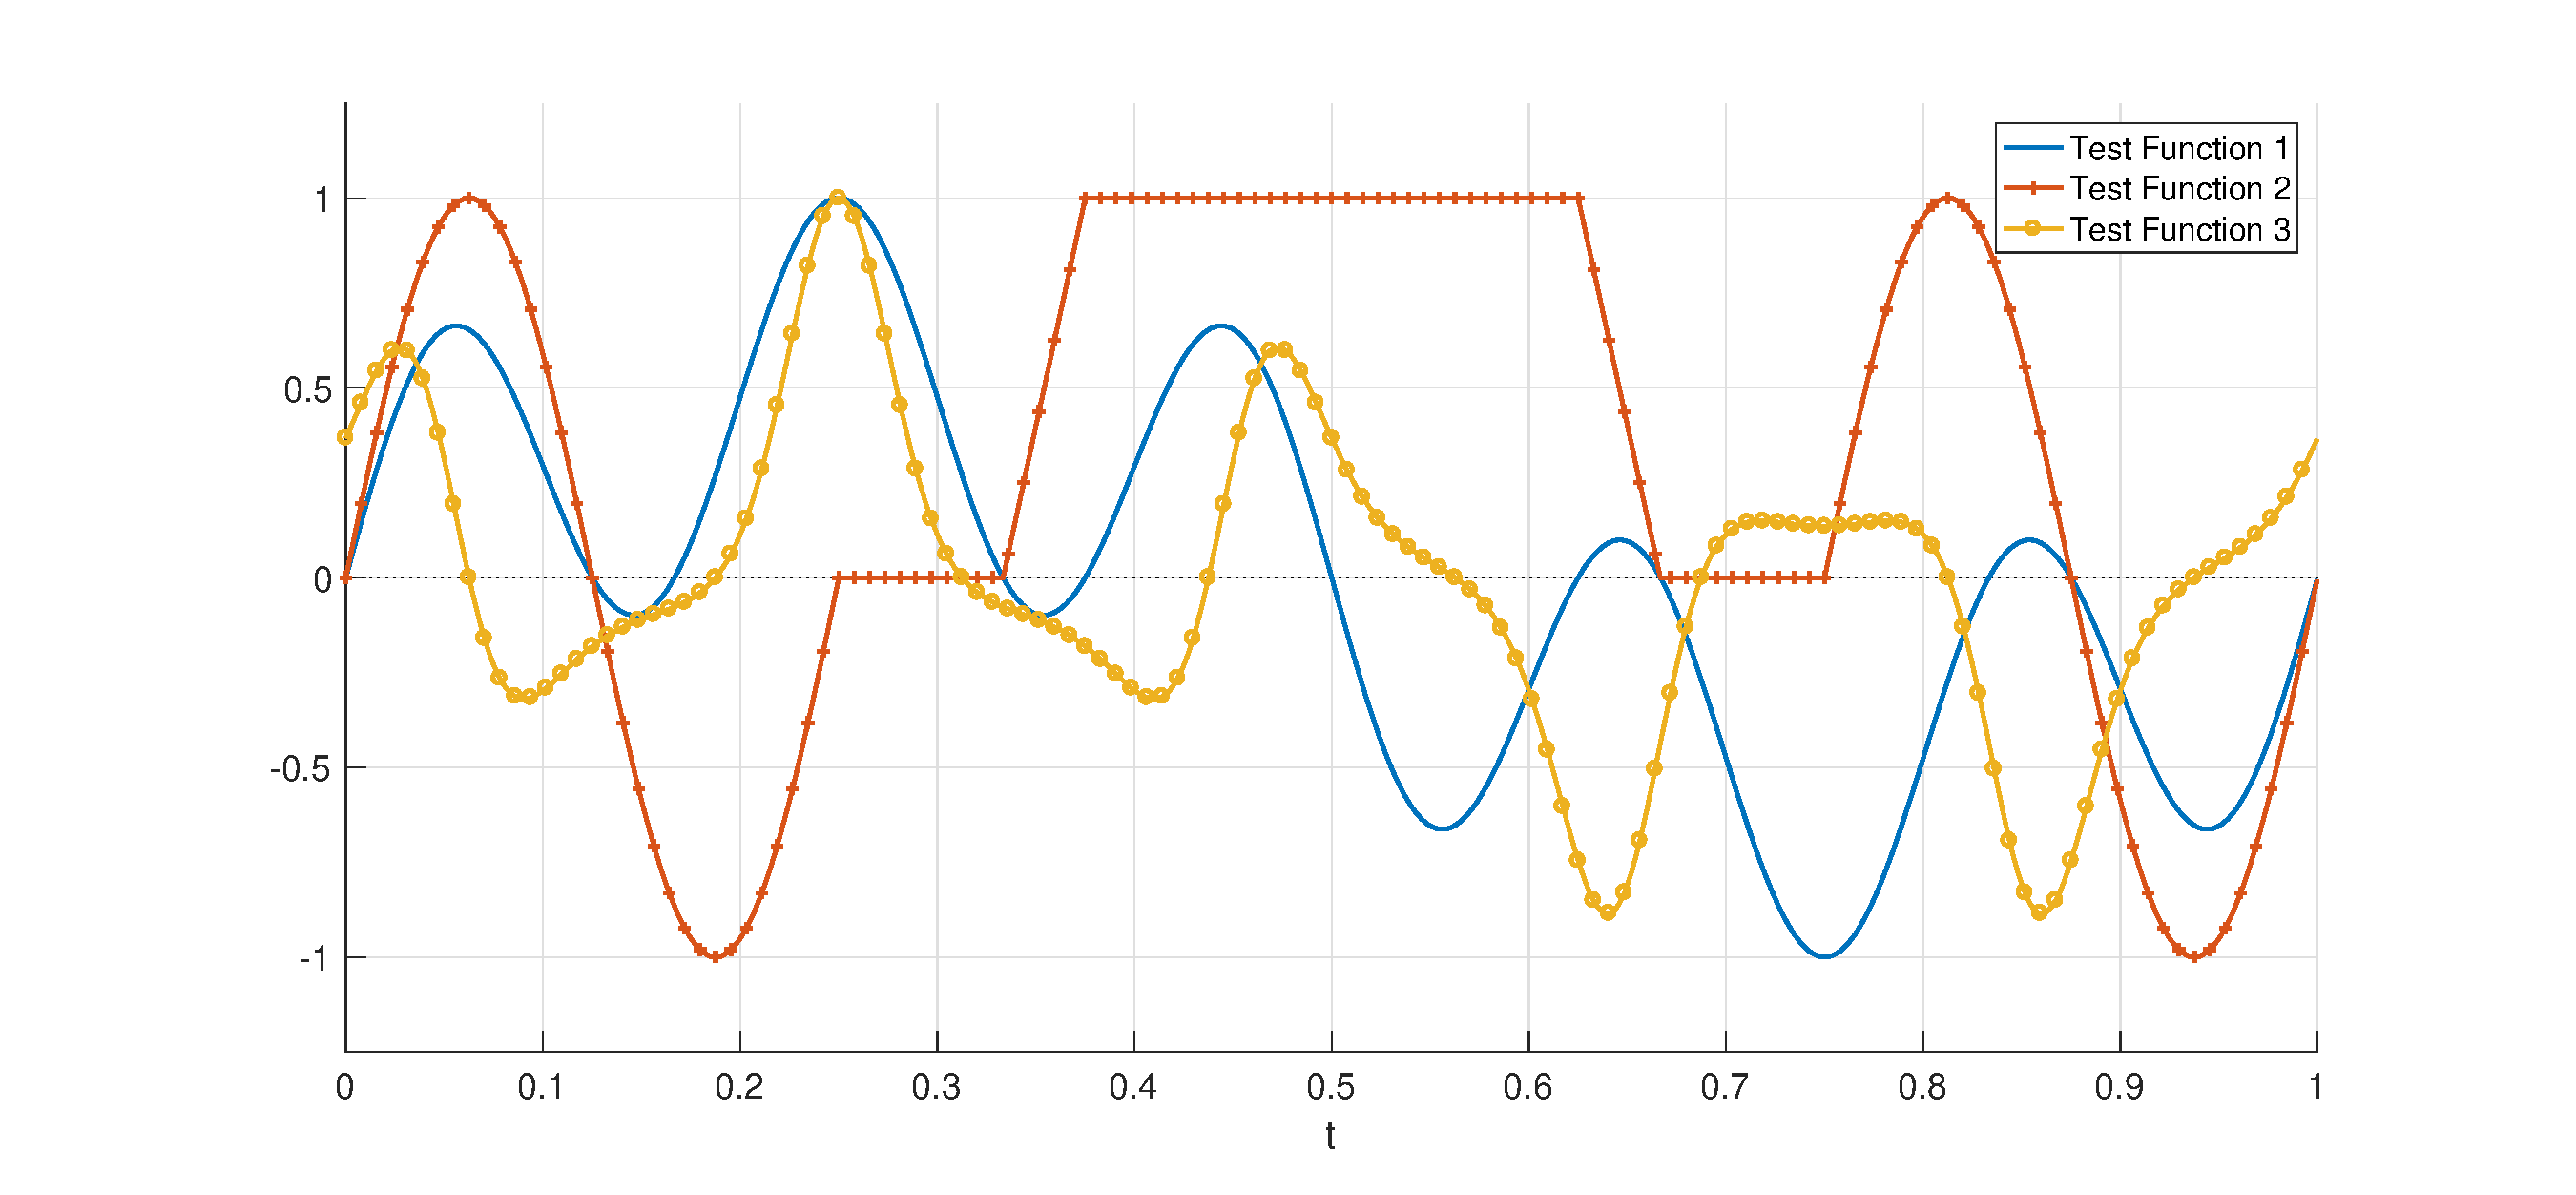
\includegraphics[scale = 0.45]{Figures/TestFunctions1D.eps}}
\caption{The three test functions considered in the numerical experiments. Note that the second test function is only piecewise-smooth, while the first and second functions are smooth. All three functions are 1-periodic.}
\label{TestFunctions}
\end{figure}

The interval $[0,1]$ is discretized as equispaced points $0, 1/N, 2/N, \ldots, (N-1)/N$ for $N = 4096$. In other words, the interval is discretized as the vector $\tVec = [t_1,t_2,\ldots,t_N]$ with $t_i = (i-1)/N$. The selected test function $f$ is then sampled at these points so that the discrete version $\fVec = [f_1,f_2,\ldots,f_N]$ has elements $f_i = f(t_i)$. For the discrete version of $k(x,t)$ to be used in the convolution with $\fVec$, the periodic extension of $k(x,t)$ is sampled in the same way that was used to construct $\fVec$. However, it is important to remember that unextended $k(x,t)$ was assumed to be centered at the origin and compactly supported on the interval $[-1/2,1/2]$. As such, a plot of $\kVec$ will not resemble the traditional graph of a Gaussian bump but instead be a depiction of a trough between bumps in the periodic extension of $k$; see Figure \ref{RegAndTroughGaussian}. In the experiments, the width of the Gaussian kernels are chosen to be 100 and 200.  \par

\begin{figure}
	\centerline{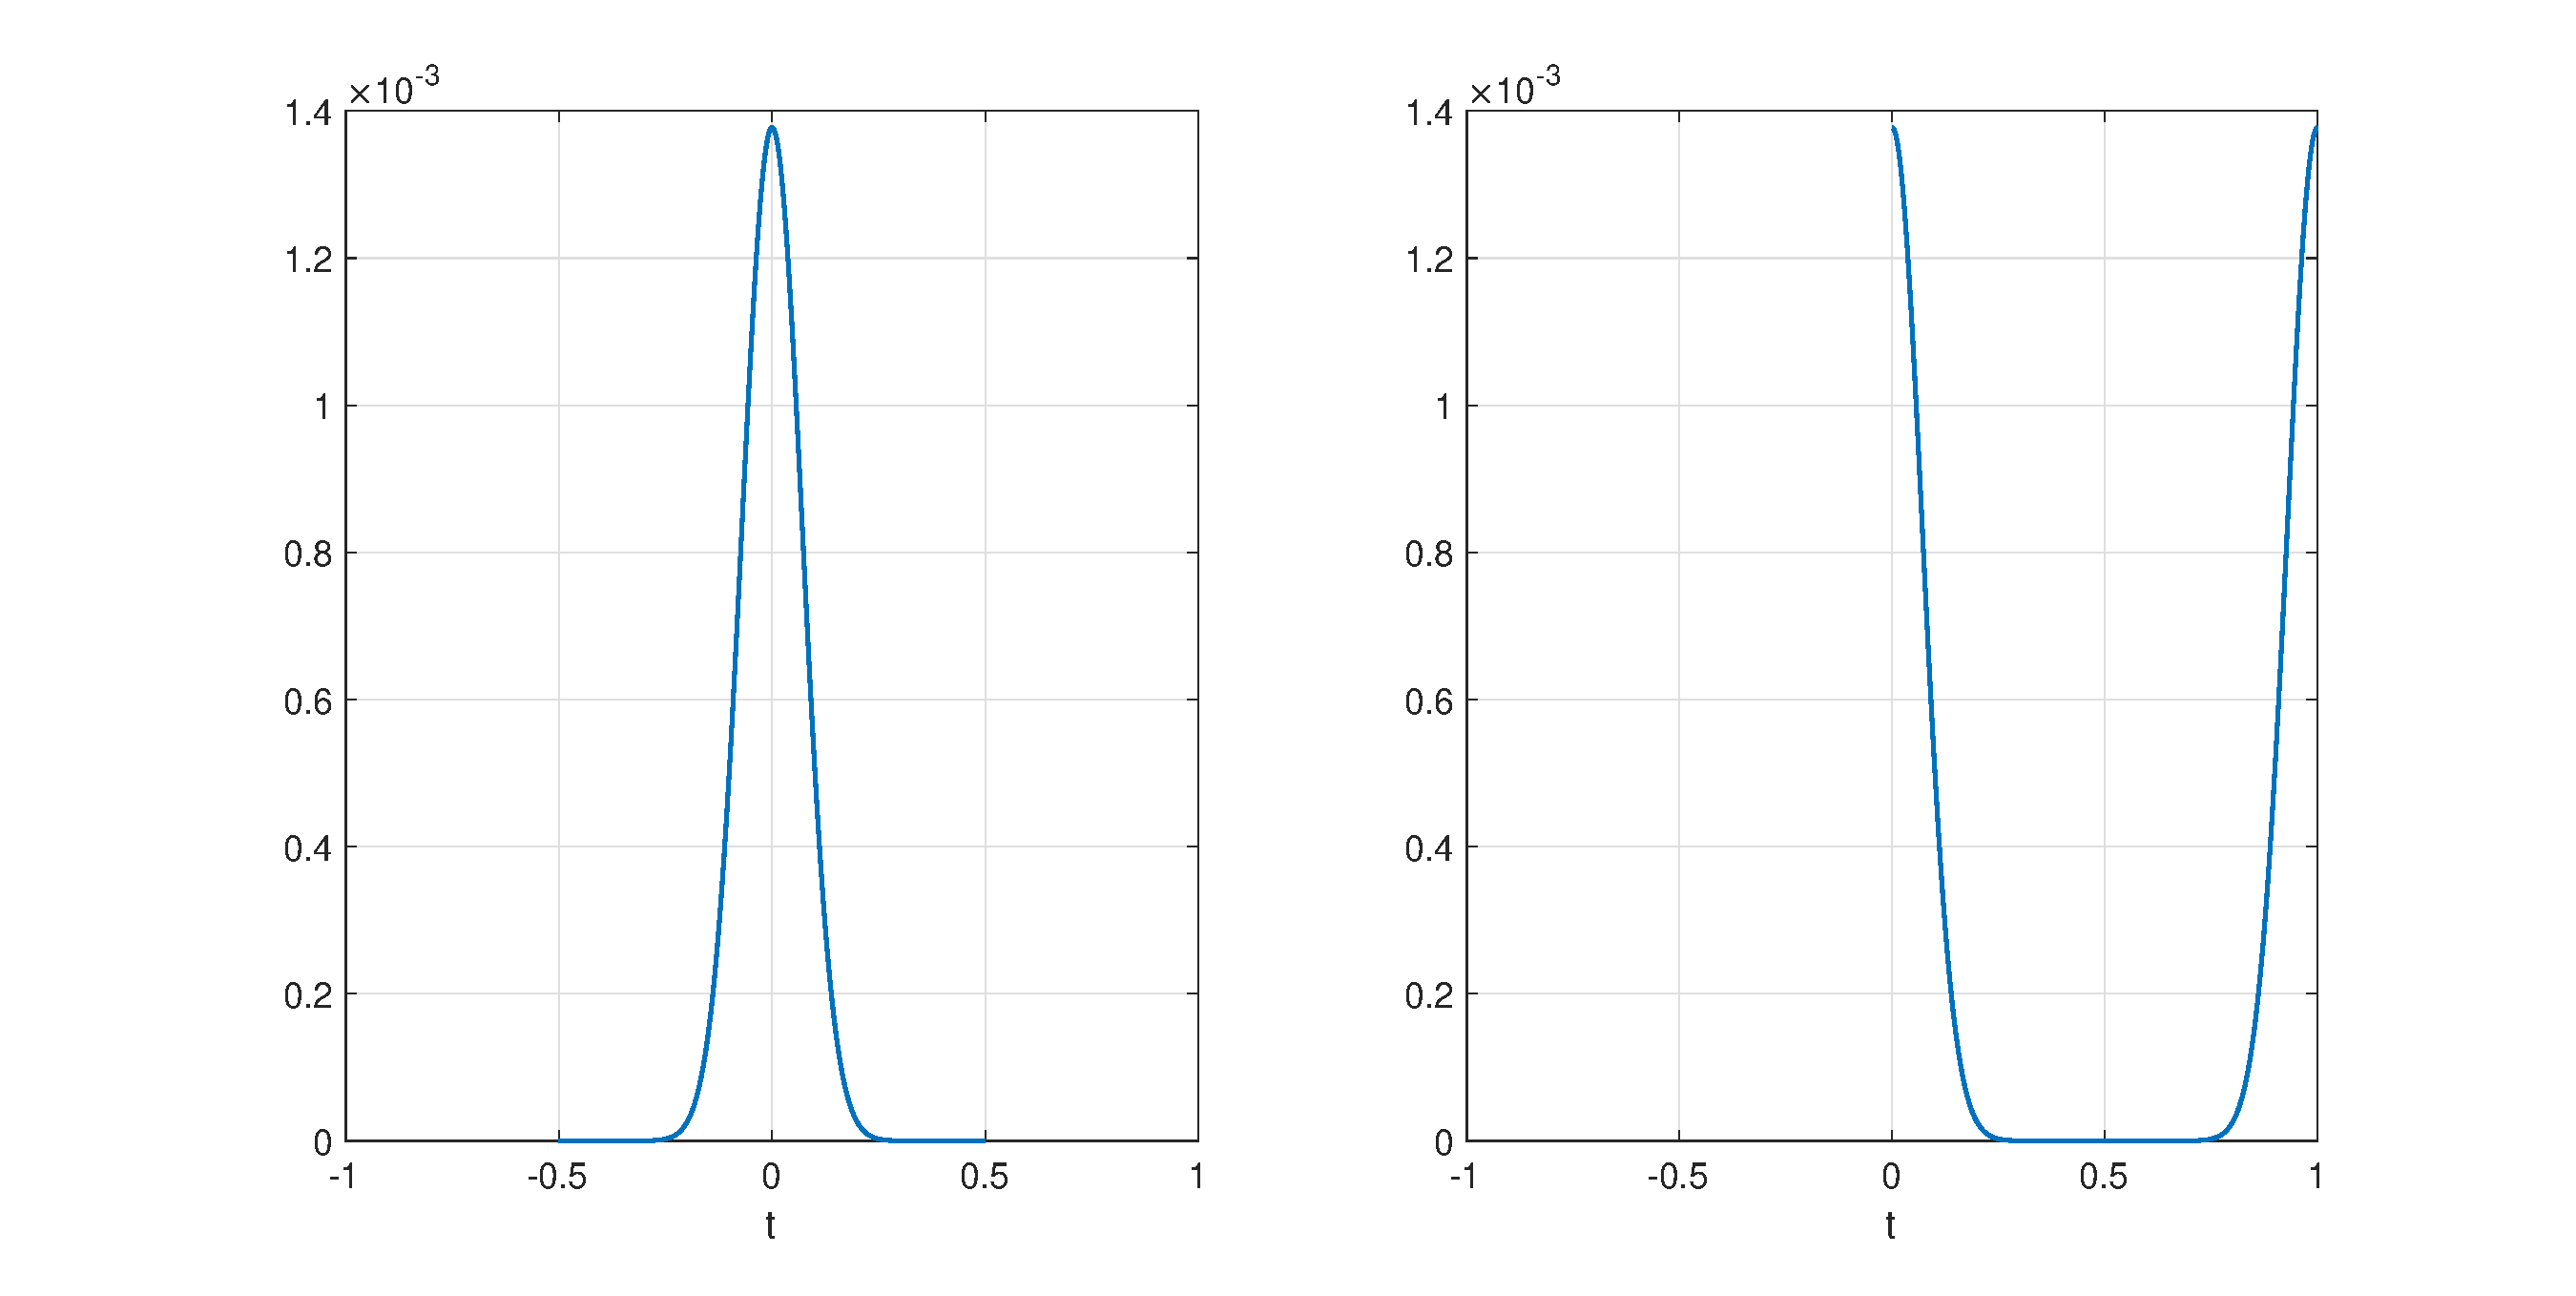
\includegraphics[scale = 0.45]{Figures/RegAndTroughGaussian.eps}}
\caption{Plots of different discretizations of the kernel $k(t)$. The discretization on the left reflects the compact support of $k(t)$ on the interval $[-1/2,1/2]$. The discretization on the right represents the periodic extension of $k(t)$ on the interval $[0,1]$.}
\label{RegAndTroughGaussian}
\end{figure}

With the discretizations $\fVec$ and $\kVec$ determined, the discretization $\gVec$ of $g(t)$ can be evaluation using either a circular convolution or a linear convolution with appropriate vector padding. Ultimately the vectors $\fVec$, $\kVec$, and $\gVec$ are vector discretizations of $f(t)$, $k(t)$, and $g(t)$, respectively. \par
Overall, two selections for the width of the Gaussian kernel, two selections 5 and 25 for SNR value, and three test functions lead to a total of 12 experimental configurations. For each configuration, 20 noise realizations were generated and tested. The full resolution problem was constructed using $N = 4096$ points. The downsamped resolutions were selected as $n \in \{16,32,\ldots,2048\}$ for a total of nine resolutions (eight values of $n$).

\subsection{Construction of noise} \label{sec:Construction of noise}

Though the definition of SNR varies, the definition chosen for this investigation is
\begin{equation}
\label{eq:SNR}
\text{SNR} = 10\log_{10}\left(\frac{P_{\text{signal}}}{P_{\text{noise}}}\right)
\end{equation}
where $P$ denotes average power. In the discrete setting, the average power of a signal $\mathbf{f}$ of length $N$ is defined as $\|\mathbf{f}\|^2/N$. Using this definition, $P_{\text{signal}} = \|\gVec\|^2/N$ and $P_{\text{noise}} = \|\noiseVec\|^2/N$ and so the quotient in the logarithm is $\|\gVec\|^2/\|\noiseVec\|^2$. The quotient can also be expressed as $(\|\gVec\|/\|\gnoiseVec - \gVec\|)^2$, which is the square of the multiplicative inverse of the relative error of $\gnoiseVec$. \par
In MATLAB, the noise vector $\noiseVec$ can be constructed by first taking an $N$-vector $\mathbf{e}$ drawn from the multivariate standard normal distribution and multiplying the vector by a constant $\noiseSD$. Doing so ensures that $\noiseVec$ has variance $\noiseSD^2$ because $\Var(\noise) = \Var(\noiseSD\:\mathbf{e}) = \noiseSD^2\:\Var(\mathbf{e})$ and $\mathbf{e}$ has unit variance. Thus it is useful to rearrange the equation defining SNR into an equation that provides a way of finding the necessary variance for a given SNR value. The rearrangement is shown below, with $\|\noiseVec\|^2$ replaced by $\E(\|\noiseVec\|^2)$.
\[\E(\|\noiseVec\|^2) = \frac{\|\gVec\|^2}{10^{(\text{SNR}/10)}}\]
Using the properties of expected value and the fact that $\E(\|\noiseVec\|^2) = \E(\|\noiseSD\:\mathbf{e}\|^2)$, the term on the left hand side of the equation can be changed as
\[\E(\|\noiseVec\|^2) = \E(\|\noiseSD\:\mathbf{e}\|^2) = \noiseSD^2 \sum_{j=1}^N \E(\mathbf{e}_i^2) = \noiseSD^2 \sum_{j=1}^N \left(\E(\mathbf{e}_i)^2 + \Var(\mathbf{e}_i)\right) = \noiseSD^2 \sum_{j=1}^N \left(0^2 + 1\right) = \noiseSD^2\:N.\]
Utilizing this change, the following equation for variance is obtained.
\begin{equation}
\label{eq:Var}
\noiseSD^2 = \frac{\|\gVec\|^2}{N \cdot 10^{(\text{SNR}/10)}}
\end{equation}
This equation is used for the numerical construction of the noise vectors. SNR values of 5 and 25 are used to generate the white noise added to $\gVec$, and one such data realization is shown in Figure \ref{NoisePlot1D_F2_S05_W200}. \par

\begin{figure}
	\centerline{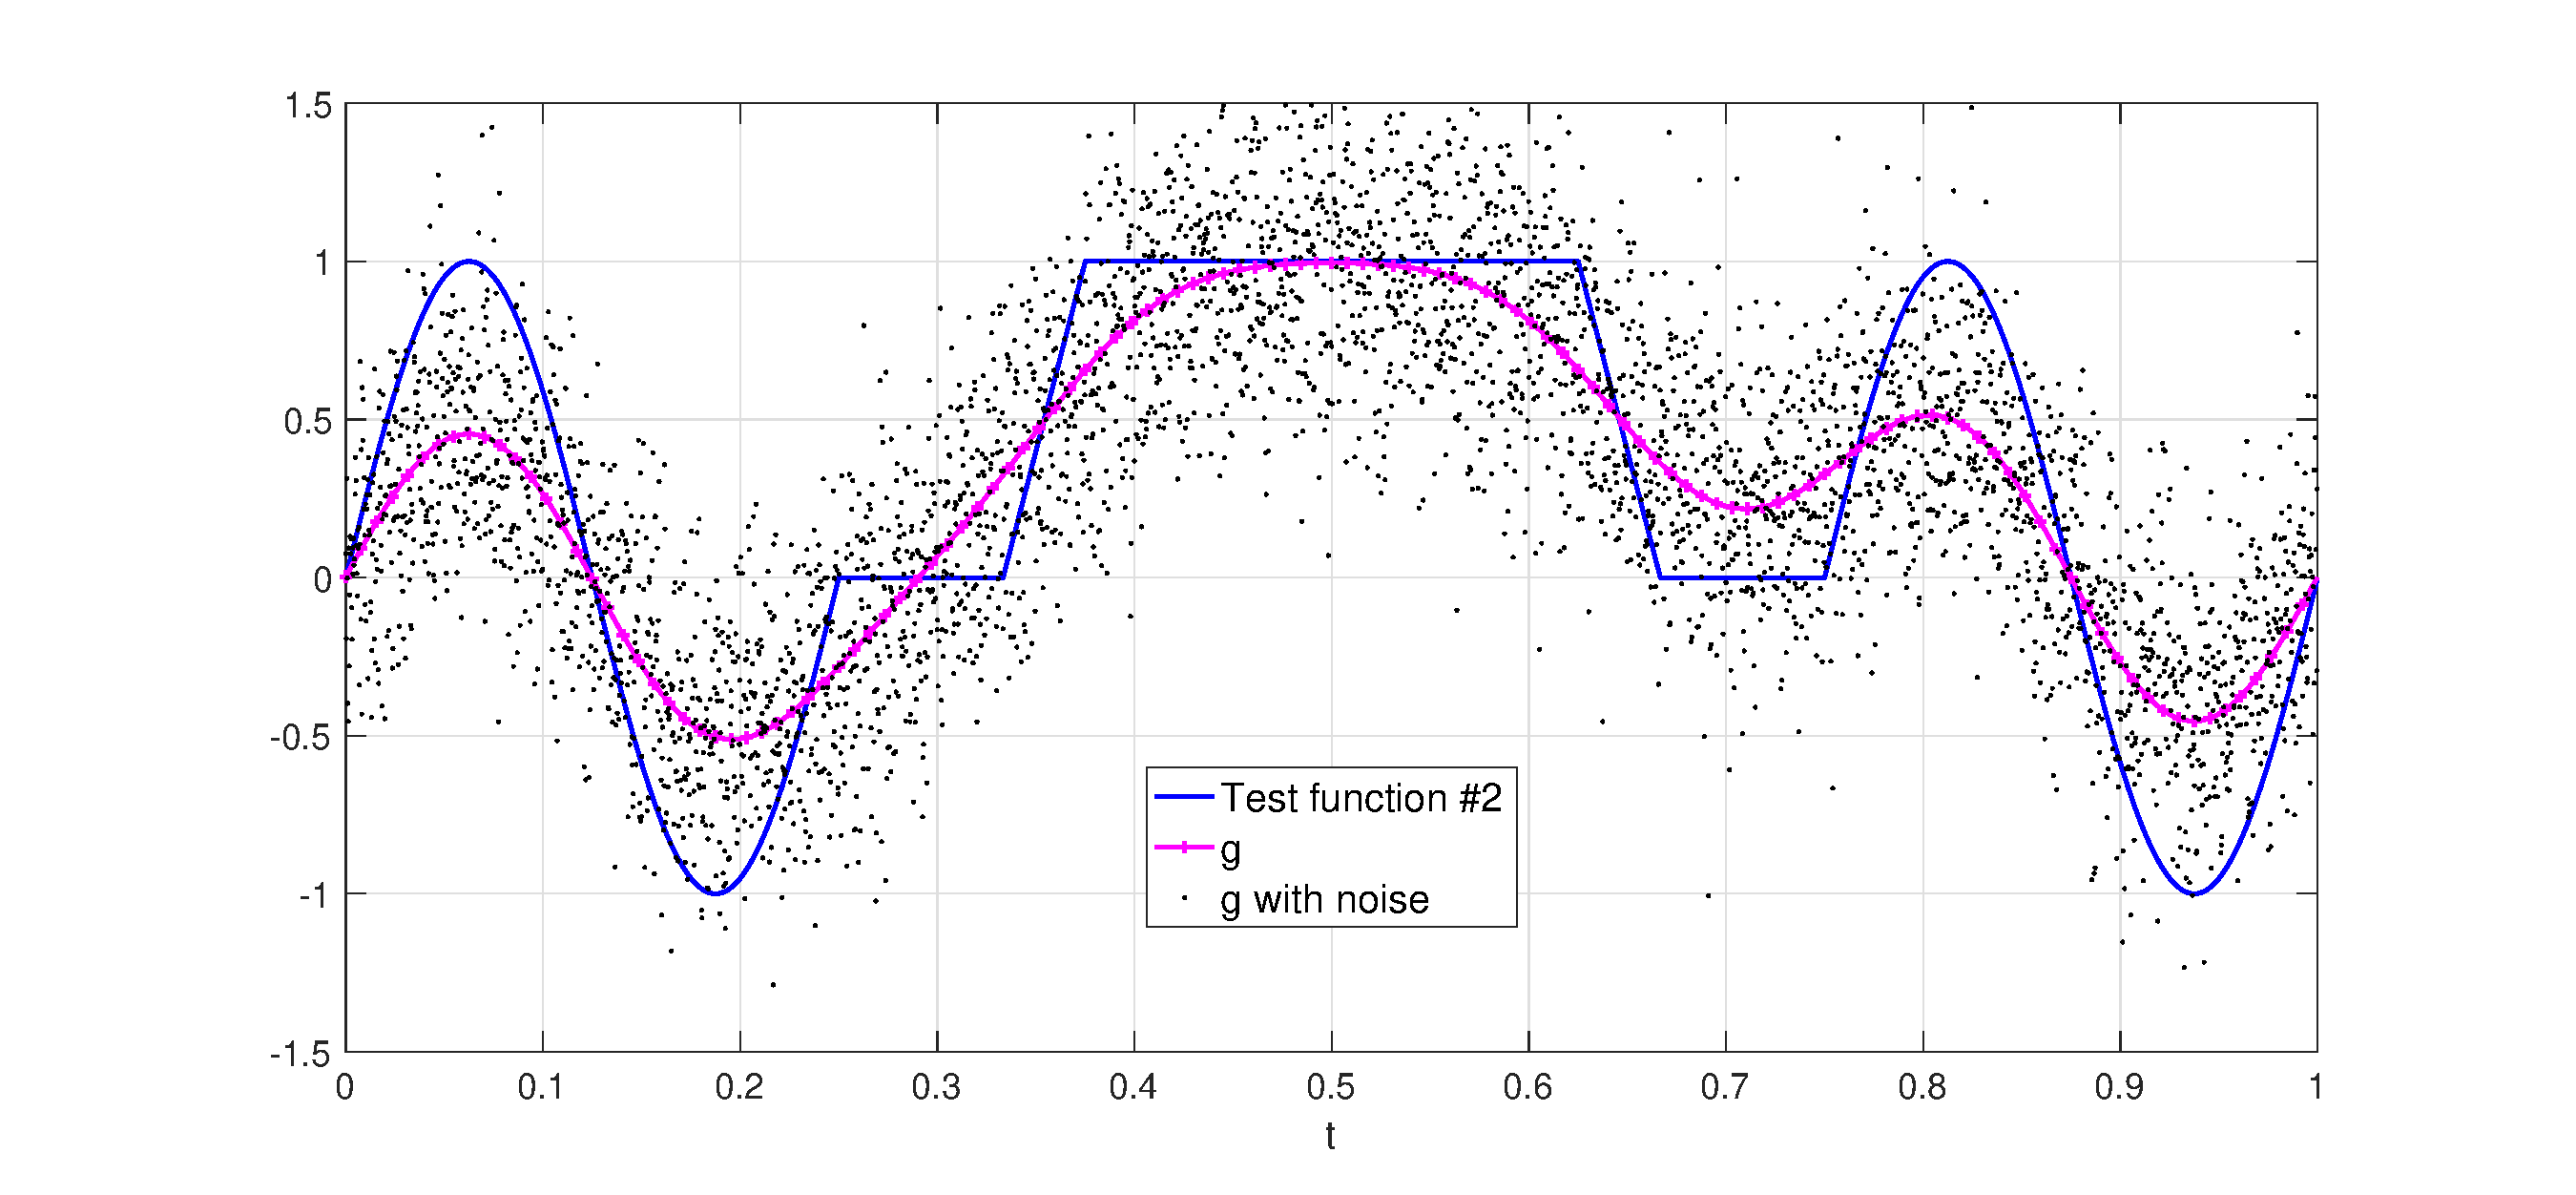
\includegraphics[scale = 0.45]{Figures/NoisePlot1D_F2_S05_W200.eps}}
\caption{The plot shows one data realization of $\gVec$ with noise, where the original function $f$ was the second test function. The SNR value is 5 and the width of the Gaussian PSF is 200.}
\label{NoisePlot1D_F2_S05_W200}
\end{figure}

For an accurate evaluation of the numerical experiments and their results, multiple realizations of noise are used. A primary advantage of multiple noise realizations is that the sample variance of noise vectors approaches the desired variance as the number of realizations increases. More rigorously, the mean of the sample variances of the noise vectors converges almost surely to the expected value of the sample variance, which is the desired variance $\noiseSD^2$; this is a direct consequence of the (strong) law of large numbers and the fact that the noise vectors are independent and identically distributed with standard normal distribution.  \par
Another numerical consideration regarding noise is how the sample variance changes across downsampling resolutions. To formalize the concept of downsampling in the context of this report, consider $\mathbf{z} = [z_1,z_2,\ldots,z_n]$. Then a vector $\mathbf{y}$ is called a downsampling of $\mathbf{z}$ if $\mathbf{y} = [z_{n_1},z_{n_2},\ldots,z_{n_m}]$, where $m \leq n$ and $n_j:\{1,2,\ldots,m\}\rightarrow\{1,2,\ldots,n\}$ is a strictly increasing function. This definition is analogous to the definition of a subsequence except with a finite number of terms. \par
Theoretically, the variance of the noise vector does not change when a vector is downsampled because of the properties of variance. For any $m\times n$ matrix $M$ and $n$-vector $\noiseVec \sim \mathcal{N}(\bm{0},\noiseSD^2I)$
\begin{equation}
\Var(M\noiseVec) = M\Var(\noiseVec)M^{\trans} = \noiseSD^2MIM^{\trans} = \noiseSD^2MM^{\trans}
\label{eq:VarProp}
\end{equation}
where $MM^\trans$ is an $m \times m$ matrix. Certainly for arbitrary $M$, $MM^\trans$ can differ from an $m \times m$ identity matrix, which would mean that the new noise vector $M\noiseVec$ no longer represents white noise. However, given an $n$-vector $\noiseVec \sim \mathcal{N}(\bm{0},\noiseSD^2I)$ and the goal of obtaining a downsampled version of $\noiseVec$, a matrix $E$ can be found such that $E\noiseVec$ is the downsampled vector. Since DFT's are utilized in the regularization process, a downsampled vector whose components are still equidistant from adjacent components is desirable. Since the finest sampling $\tVec$ of the interval $[0,1]$ has $N = 4096 = 2^{12}$ points, a natural downsampling with this property would be to select every other component of $\tVec$. The resulting downsampled vector would then have length $N/2 = 2048 = 2^{11}$. The matrix $E$ that accomplishes this downsampling is the $N/2 \times N$ matrix defined as
\begin{equation}
E = [\mathbf{e}_1 \: \mathbf{0} \: \mathbf{e}_2 \: \mathbf{0} \: \mathbf{e}_3 \: \mathbf{0} \ldots \mathbf{e}_N]
\label{eq:Downsampling matrix}
\end{equation}
where $\mathbf{0}$ is the $N/2$-vector of all zeros and $\mathbf{e}_j$ is the $N/2$-vector of all zeros except for 1 as the $j\text{th}$ component, $1 \leq j \leq N/2$. Another explanation of how to construct $E$ is to concatenate every other row of an $N \times N$ identity matrix. In an effort to clarify this downsampling process, let $\tVec^{n}$ denote the $n$-point downsampling of $\tVec$. Then with this new notation, $\tVec^{2046} = E\tVec$. \par
As a smaller example, consider the vector
\[\tVec = \begin{bmatrix}
0 & \dfrac{1}{8} & \dfrac{1}{4} & \dfrac{3}{8} & \dfrac{1}{2} & \dfrac{5}{8} & \dfrac{3}{4} & \dfrac{7}{8}
\end{bmatrix}^{\trans},\]
which is an equispaced 8-point discretization of $[0,1]$. The $4 \times 8$ matrix $E$ used to obtain downsampling $\tVec^{4}$ is
\[E = \begin{bmatrix}
1 & 0 & 0 & 0 & 0 & 0 & 0 & 0 \\
0 & 0 & 1 & 0 & 0 & 0 & 0 & 0 \\
0 & 0 & 0 & 0 & 1 & 0 & 0 & 0 \\
0 & 0 & 0 & 0 & 0 & 0 & 1 & 0 \\
\end{bmatrix}.\]
Then $\tVec^4$ obtained by the product $E\tVec$ has equispaced components as desired:
\[\tVec^4 = E\tVec = \begin{bmatrix}
0 & \dfrac{1}{4} & \dfrac{1}{2} & \dfrac{3}{4}
\end{bmatrix}^{\trans}.\]
\indent Another property of the $N/2 \times N$ matrix $E$ defined in \eqref{eq:Downsampling matrix} is that $EE^{\trans} = I$, where $I$ is the $N/2 \times N/2$ identity matrix.  This is a direct consequence of $\mathbf{e}_j\mathbf{e}_j^\trans = 1$ for all $j$ with $1 \leq j \leq N/2$. Using the property in \eqref{eq:VarProp}, the variance of the  noise vector $\noiseVec^{N/2}$ downsampled from $\noiseVec$ is then
\[\Var(\noiseVec^{N/2}) = \Var(E\noiseVec) = E\Var(\noiseVec)E^{\trans} = \noiseSD^2EE^{\trans} = \noiseSD^2I\]
where $I$ is the $N/2 \times N/2$ identity matrix. Therefore, downsampling white noise vectors in this way produces white noise vectors of half length, theoretically preserving variance across downsamples. As a final remark, the process of downsampling described here can be used to obtain downsampled vectors of length $N/(2^2), N/(2^3), \ldots, N/N$, though the final resolution in this report has been chosen as $N/(2^8) = 16$. \par 
While the variance of the noise is preserved across downsampling resolution in theory, numerically there is some fluctuation. As the downsampling resolutions decrease, i.e. the length of the downsampled vectors decreases, the sample variances more spread out. Figure \ref{VarPlot1D} demonstrates this phenomenon by showing boxplots of sample variance versus downsampling resolutions. \newpage

\begin{figure}[htb]
\centerline{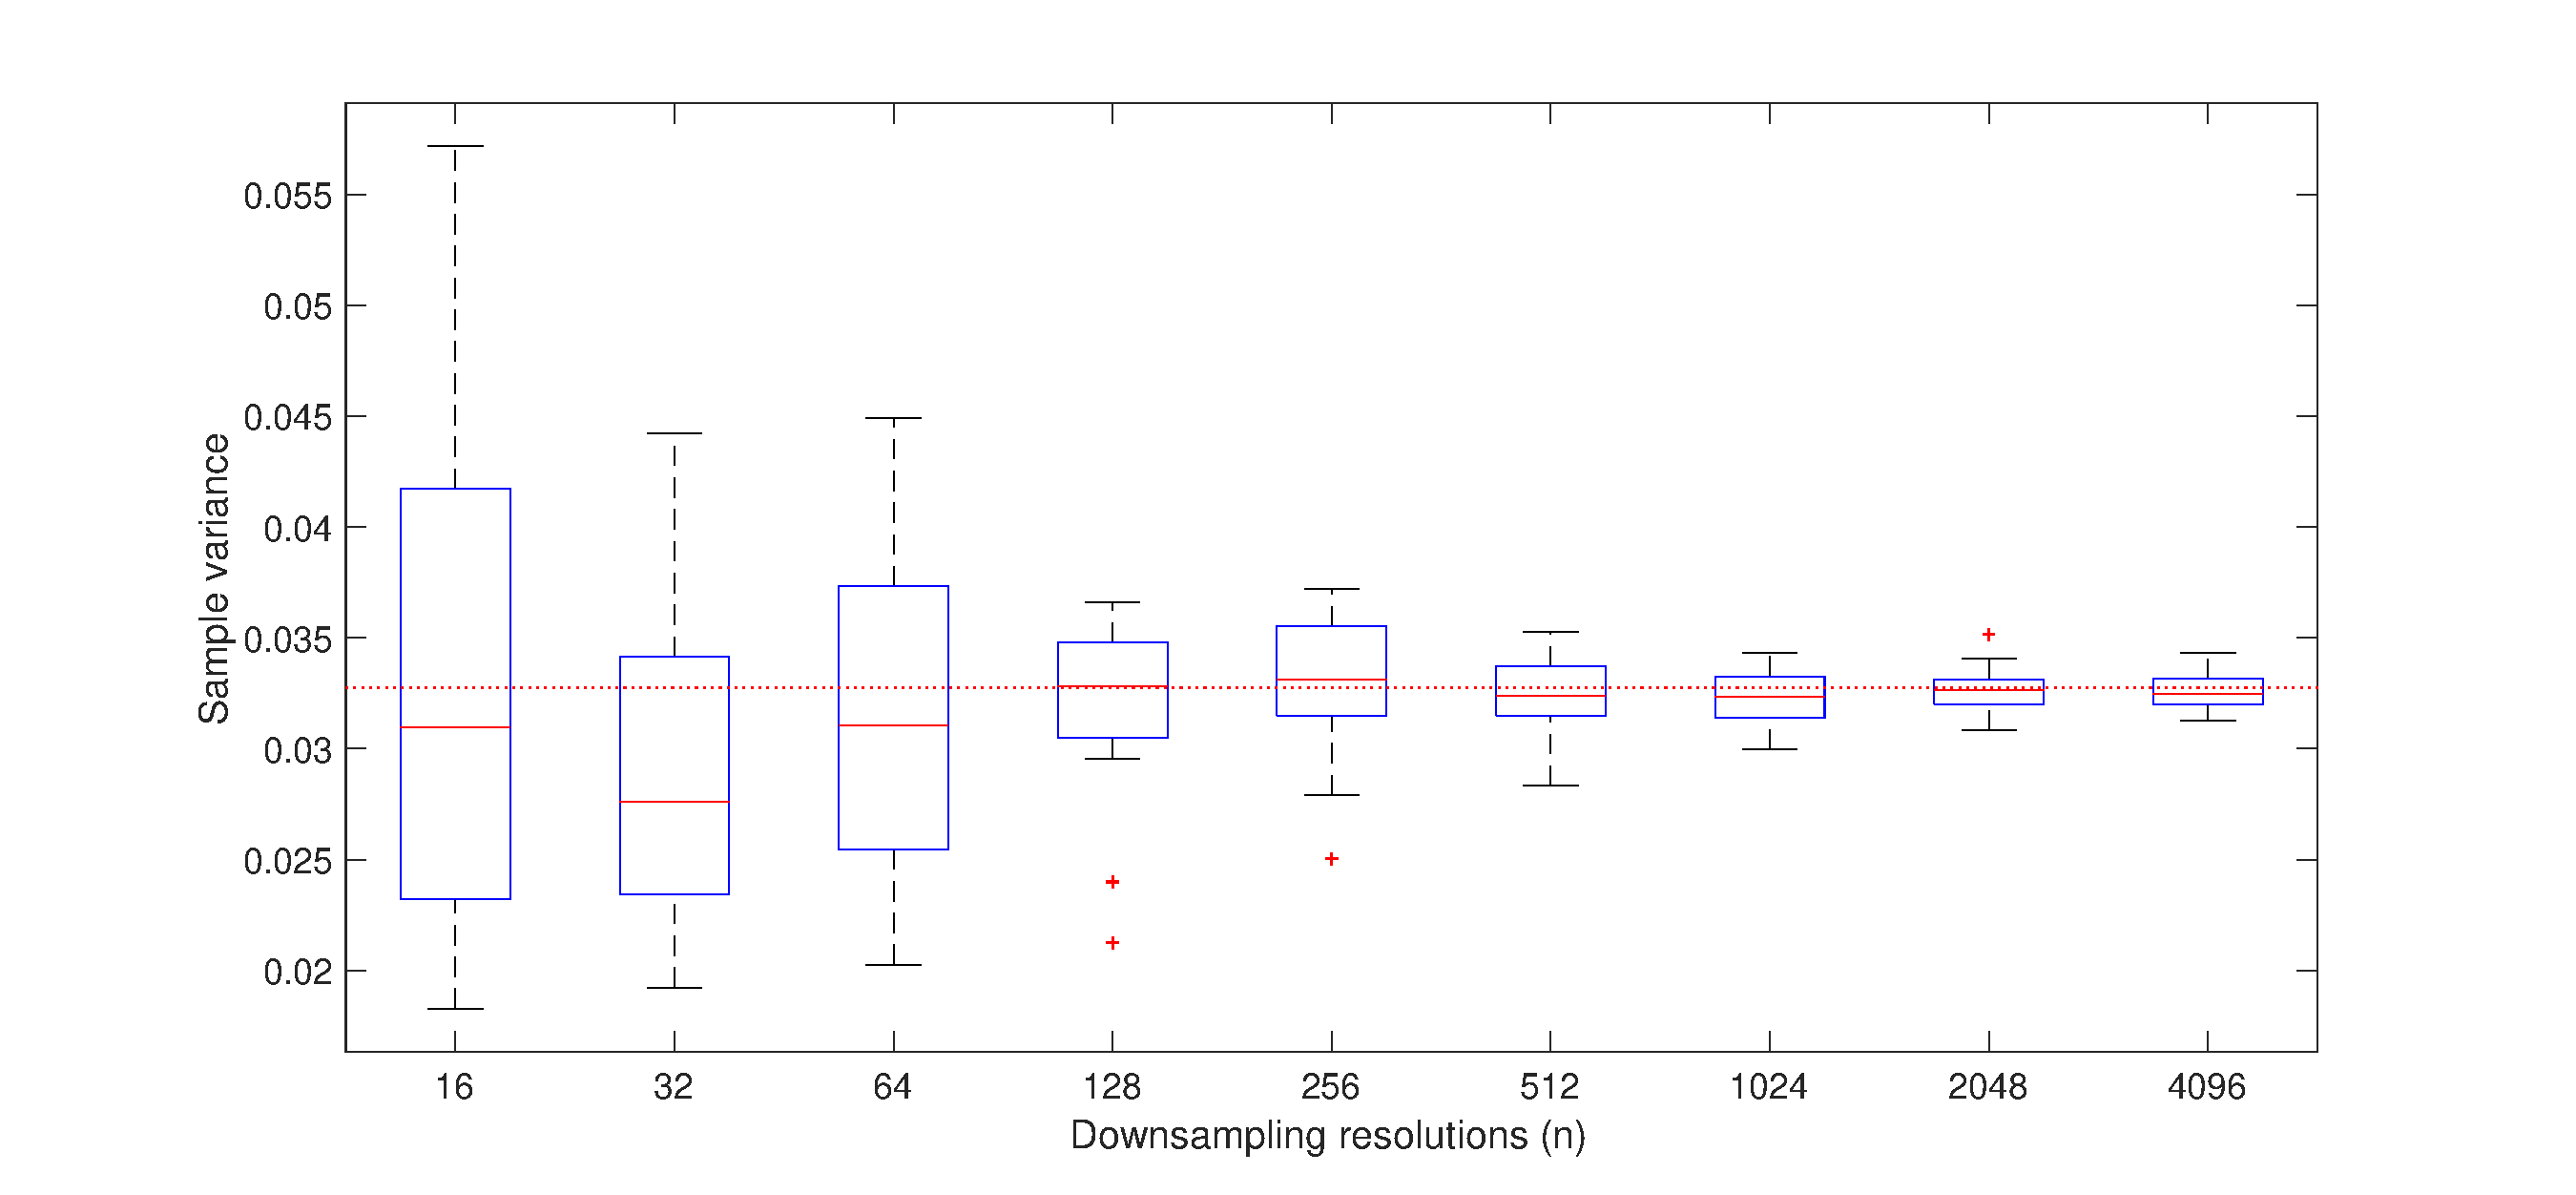
\includegraphics[scale=0.45]{Figures/VarPlot1D_F1_S05_W100_R20.eps}}
\caption{The boxplots were generated from the sample variances of downsampled noise vectors. The theoretical variance of the noise was set to 0.0327, which is indicated by the horizontal dotted line. This figure illustrates that as the lengths of the downsampled vectors decrease, the variance in the computed sample variances increases.}
\label{VarPlot1D}
\end{figure}

\section{Parameter estimation methods} \label{sec:Parameter estimation methods}

Perhaps the simplest method of selecting a regularization parameter is to use
\begin{equation}
\regparam_{\text{best}} := \argmin_{\regparam \geq 0} \|\fVec - \freg\|^2.
\label{eq:Minimize Error}
\end{equation}
Here ``best'' is used to indicate the fact that the parameter is chosen to minimize the error of the regularized solution. The primary disadvantage of using this method is that the true solution $\fVec$ must be known. Not only would knowing the true solution render the process of finding a regularized solution pointless, but in practice a true solution is not known. This motivates the use of other methods, which do not rely upon knowledge of a true solution. The three such methods considered in this report are the Unbiased Predictive Risk Estimator method (Section \ref{sec:Unbiased Predictive Risk Estimator}), the Generalized Cross Validation method (Section \ref{sec:Generalized Cross Validation}), and the Discepancy Principle method (Section \ref{sec:Discrepancy Principle}). Since true solutions are known for use in the numerical experiments, the method on line \eqref{eq:Minimize Error} will be used as a benchmark for comparing the other three methods.

\subsection{Unbiased Predictive Risk Estimator} \label{sec:Unbiased Predictive Risk Estimator}
The Unbiased Predictive Risk Estimator (UPRE) method is derived by considering the quantity
\[\PE := \kMat(\freg - \fVec).\]
This quantity $\PE$ is known as the \textit{predictive error}, and is an alternative to solution error defined as $\freg - \fVec$. Given the above definition, the mean squared norm of the predictive error is
\[\frac{1}{n}\|\PE\|^2 = \frac{1}{n}\|\kMat(\freg - \fVec)\|^2\]
which is called the predictive risk.  As a first step in deriving the UPRE method, assume that the noise $\noiseVec$ is a random vector, instead of a realization of a random vector. Direct consequences of this assumption are that $\gVec$ and $\freg$ are random vectors and the predictive risk $(1/n)\|\PE\|^2$ is a random variable. \par
Next, an $n \times n$ matrix $\A$ is defined as $\A = \kMat\R$ where $\R$ is a regularization matrix. The notation $\A$ is chosen to indicate that the matrix depends upon the regularization parameter contained in $\R$. Using the influence matrix with $\freg = \R\gnoiseVec$, the predictive error can be rewritten:
\begin{align*}
\PE &= \kMat\freg - \kMat\fVec \\
&= \A\gnoiseVec - \kMat\fVec \\
&= \A(\kMat\fVec + \noiseVec) - \kMat\fVec \\
&= (\A - I)\kMat\fVec + \A\noiseVec
\end{align*}
By the assumption that $\noiseVec$ is a discrete white noise vector, the Trace Lemma can be utilized to obtain an expression for the expected value of predictive risk.

\begin{TL}
Let $f \in \mathcal{H}$, where $\mathcal{H}$ is a deterministic, real Hilbert space, let $\noiseVec$ be a discrete noise vector with $\noiseVec \sim \mathcal{N}(0,\noiseSD^2)$, and let $B: \mathbb{R}^n \rightarrow \mathcal{H}$ be a bounded linear operator. Then
\[\E(\|f + B\noise\|_{\mathcal{H}}^2) = \|f\|_{\mathcal{H}}^2 + \noiseSD^2\trace({B^*}B)\]
where $B^*$ denotes the adjoint of $B$.
\end{TL}
\begin{proof}
By the linearity of inner products and the expected value operator,
\[\E(\|f + B\noiseVec\|_{\mathcal{H}}^2) = \E(\langle f + B\noiseVec, f + B\noiseVec\rangle_{\mathcal{H}}) = \E(\|f\|_{\mathcal{H}}^2) + 2\E(\langle f, B\noiseVec\rangle_{\mathcal{H}}) + \E(\langle B\noiseVec, B\noiseVec\rangle_{\mathcal{H}}).\]
The term $\E(\|f\|_{\mathcal{H}}^2)$ reduces to $\|f\|_{\mathcal{H}}^2$ because $f$ is an element of a deterministic Hilbert space. Next, the inner products can be rewritten using the adjoint of $B$:
\begin{align*}
\E(\|f + B\noiseVec\|_{\mathcal{H}}^2) &= \|f\|_{\mathcal{H}}^2 + 2\E(\langle f, B\noiseVec\rangle_{\mathcal{H}}) + \E(\langle B\noiseVec, B\noiseVec\rangle_{\mathcal{H}}) \\
&= \|f\|_{\mathcal{H}}^2 + 2\E(({B^*}f)^\trans\noiseVec) + \E({\noiseVec^\trans}{B^*}B\noiseVec) \\
&= \|f\|_{\mathcal{H}}^2 + 2\sum_{j=1}^n ({B^*}f)_j \E(\noise_j) + \sum_{j=1}^n\sum_{k=1}^n ({B^*}B)_{jk} \E({\noise_j}{\noise_k})
\end{align*}
Since $\noiseVec \sim \mathcal{N}(0,\noiseSD^2)$, the expected values of $\noise_j$ and ${\noise_j}{\noise_k}$ are zero and $\noiseSD^2\delta_{jk}$, respectively. Therefore the second term above is zero and the third term is a summation expression for $\noiseSD^2\trace({B^*}B)$.
\end{proof}

\noindent Applying the Trace Lemma to the expression for predictive risk yields
\[\E\left(\frac{1}{n}\|\PE\|^2\right) = \frac{1}{n}\E\left(\|(\A-I)\kMat\fVec + \A\noiseVec\|^2\right) = \frac{1}{n}\|(\A-I)\kMat\fVec\|^2 + \frac{\noiseSD^2}{n}\trace({\A^\trans}\A).\]
If Tikhonov regularization is used, then the influence matrix $\A$ is $\kMat(\kMat^\ctrans\kMat + \regparam{D^\ctrans}D)^{-1}\kMat^\ctrans$. The matrix $(\kMat^\ctrans\kMat + \regparam{D^\ctrans}D)^{-1}$ is symmetric as a result of $\kMat^\ctrans\kMat$ and $\regparam{D^\ctrans}D$ being individually symmetric, and thus the corresponding influence matrix $\A$ is symmetric.  With a symmetric matrix $\A$, the expected value of predictive risk is simplified to
\begin{equation}
\label{eq:PR}
\E\left(\frac{1}{n}\|\PE\|^2\right) = \frac{1}{n}\|(\A-I)\kMat\fVec\|^2 + \frac{\noiseSD^2}{n}\trace(\A^2).
\end{equation}
\indent The last step in the derivation of the UPRE method is to introduce the \textit{regularized residual}, which is defined as $\regres = \kMat\freg - \gnoiseVec$. The regularized residual is important because it is also used in the derivation of the generalized cross validation and discrepancy principle methods. Using the influence matrix $\A$, the expression for $\regres$ can also be written as
\[\regres = (\A-I)\gnoiseVec = (\A-I)(\kMat\fVec + \noiseVec) = (\A-I)\kMat\fVec + (\A-I)\noiseVec.\]
By the Trace Lemma and the expression for $\regres$, the expected value of $(1/n)\|\regres\|^2$ is
\[\E\left(\frac{1}{n}\|\regres\|^2\right) = \frac{1}{n}\|(\A-I)\kMat\fVec\|^2 + \frac{\noiseSD^2}{n}\trace({(\A-I)^\trans}(\A-I))\]
For symmetric $\A$, the term $(\A-I)^\trans(\A-I)$ becomes $(\A-I)^2 = \A^2 - 2\A + I$ and so by the linearity of the trace operator,
\begin{equation}
\label{eq:RR}
\E\left(\frac{1}{n}\|\regres\|^2\right) = \frac{1}{n}\|(\A-I)\kMat\fVec\|^2 + \frac{\noiseSD^2}{n}\trace(\A^2) - \frac{2\noiseSD^2}{n}\trace(\A) + \noiseSD^2.
\end{equation}
By comparing \eqref{eq:PR} and \eqref{eq:RR}, the equation for the expected value of $(1/n)\|\PE\|^2$ can be expressed as
\[\E\left(\frac{1}{n}\|\PE\|^2\right) = \E\left(\frac{1}{n}\|\regres\|^2\right) + \frac{2\noiseSD^2}{n}\trace(\A) - \noiseSD^2.\]
The UPRE is defined to be
\begin{equation}
\label{eq:UPRE}
\U(\regparam) = \frac{1}{n}\|\regres\|^2 + \frac{2\noiseSD^2}{n}\trace(\A) - \noiseSD^2
\end{equation}
and the UPRE method is to pick $\regparam_{\text{UPRE}} = \argmin_{\regparam \geq 0} \U(\regparam)$. \par 
Since the DFT is a the primary tool in the experiment, a spectral form of the UPRE function (one that involves DFT's) is desirable, as are spectral forms of the GCV and discrepancy principal functions in Sections \ref{sec:Generalized Cross Validation} and \ref{sec:Discrepancy Principle}. To derive a spectral form of \eqref{eq:UPRE}, first recall that for Tikhonov regularization, $\A = \kMat(\kMat^\ctrans\kMat + \regparam{D^\ctrans}D)^{-1}\kMat^\ctrans$. From \eqref{eq:CircDiag}, $\kMat = F^*\Delta{F}$, where $\Delta = \diag(\widehat{\kVec})$. If $D = F^\ctrans\Lambda{F}$ as well (with $\Lambda = \diag(\widehat{\dVec})$), then
\begin{align*}
\A &= \kMat(\kMat^\ctrans\kMat + \regparam{D^\ctrans}D)^{-1}\kMat^\ctrans \\
&= F^*\Delta{F}((F^*\Delta{F})^\ctrans F^\ctrans\Delta{F} + \regparam(F^\ctrans\Lambda{F})^\ctrans F^\ctrans\Lambda{F})^{-1}(F^*\Delta{F})^\ctrans \\
&= F^\ctrans\Delta{F}(F^\ctrans\Delta^\ctrans\Delta{F} + \regparam{F^\ctrans\Lambda^\ctrans\Lambda{F}})^{-1}F^\ctrans\Delta^\ctrans{F} \\
&= F^\ctrans\Delta{F}(F^\ctrans(\Delta^\ctrans\Delta + \regparam\Lambda^\ctrans\Lambda)F)^{-1}F^\ctrans\Delta^\ctrans{F} \\
&= F^\ctrans\Delta{F}F^\ctrans(\Delta^\ctrans\Delta + \regparam\Lambda^\ctrans\Lambda)^{-1}FF^\ctrans\Delta^\ctrans{F} \\
&= F^\ctrans\Delta(\Delta^\ctrans\Delta + \regparam\Lambda^\ctrans\Lambda)^{-1}\Delta^\ctrans{F}.
\end{align*}
The matrix $\Delta(\Delta^\ctrans\Delta + \regparam\Lambda^\ctrans\Lambda)^{-1}\Delta^\ctrans$ is diagonal, and so its diagonal entries are the the eigenvalues of $\A$. Then by definition of $\Delta$ and $\Lambda$, the $j$th diagonal entry of $\Delta(\Delta^\ctrans\Delta + \regparam\Lambda^\ctrans\Lambda)^{-1}\Delta^\ctrans$ is $|\widehat{k}_j|^2/(|\widehat{k}_j|^2 + \regparam|\widehat{d}_j|^2)$. Therefore,
\begin{equation}
\trace(\A) = \sum_{j = 0}^{n-1} \frac{|\widehat{k}_j|^2}{|\widehat{k}_j|^2 + \regparam|\widehat{d}_j|^2} = \sum_{j = 0}^{n-1} \filt(\regparam,|\widehat{k}_j|)
\label{eq:TraceUPRE}
\end{equation}
where $\filt$ is the Tikhonov filter function \eqref{eq:TikFilt}. Since the operator $D$ is fixed, the vector $\widehat{\dVec}$ can be pre-computed; this is reflected by the notation $\filt(\regparam,|\widehat{k}_j|)$. \par
Next, the definition of $\regres$ gives
\[\frac{1}{n}\|\regres\|^2 = \frac{1}{n}\|\kMat\freg - \gnoiseVec\|^2 = \sum_{j = 0}^{n-1} |\widehat{k}_j\widehat{(\freg)}_j - \widehat{\gnoise}_j|^2,\]
and \eqref{eq:TikFiltPsi} and \eqref{eq:TikSol} then produce
\begin{equation}
\frac{1}{n}\|\regres\|^2 = \sum_{j = 0}^{n-1} |\filt(\regparam,|\widehat{k}_j|)\widehat{\gnoise}_j - \widehat{\gnoise}_j|^2 = \sum_{j = 0}^{n-1} |\widehat{\gnoise}_j|^2(\mfilt(\regparam,|\widehat{k}_j|))^2.
\label{eq:RegResNorm}
\end{equation}
Combining \eqref{eq:TraceUPRE} and \eqref{eq:RegResNorm} produces the spectral from of the UPRE function:
\begin{equation}
\U(\regparam) = \sum_{j = 0}^{n-1} |\widehat{\gnoise}_j|^2(\mfilt(\regparam,|\widehat{k}_j|))^2 + \frac{2\noiseSD^2}{n}\sum_{j = -0}^{n-1} \filt(\regparam,|\widehat{k}_j|) - \noiseSD^2.
\label{eq:SpectralUPRE}
\end{equation} 
Since the UPRE method relies on finding a minimum of \eqref{eq:SpectralUPRE}, the constant $\noiseSD^2$ can be ignored during implementation. In an effort to be more descriptive (note that \eqref{eq:SpectralUPRE} also relies upon $n$), define
\begin{equation}
\U_n(\regparam) = \sum_{j = 0}^{n-1} |\widehat{\gnoise}_j|^2(\mfilt(\regparam,|\widehat{k}_j|))^2 + \frac{2\noiseSD^2}{n}\sum_{j = 0}^{n-1} \filt(\regparam,|\widehat{k}_j|).
\label{eq:SpectralUPREn}
\end{equation}
The problem of finding a minimizer of \eqref{eq:SpectralUPREn} can be recast as a root-finding problem by using the derivative of the UPRE function, which is
\begin{equation}
\U'_n(\regparam) = 2\regparam^2\left[\sum_{j = 0}^{n-1} \frac{|\widehat{\gnoise}_j|^2|\widehat{k}_j|^2}{(|\widehat{k}_j|^2 + \regparam^2)^3} - \frac{2\noiseSD^2}{n}\sum_{j = 0}^{n-1} \frac{|\widehat{k}_j|^2}{(|\widehat{k}_j|^2 + \regparam^2)^2}\right].
\label{eq:SpectralUPREnDeriv}
\end{equation}
It is clear that $\regparam = 0$ is a root of \eqref{eq:SpectralUPREnDeriv} regardless of the data and operator spectra, so this root should be ignored (since a solution generated for $\regparam = 0$ is in fact a non-regularized solution). Therefore any meaningful regularization parameter selected from the UPRE method will be a root of
\begin{equation}
V_n(\regparam) := \sum_{j = 0}^{n-1} \frac{|\widehat{\gnoise}_j|^2|\widehat{k}_j|^2}{(|\widehat{k}_j|^2 + \regparam^2)^3} - \frac{2\noiseSD^2}{n}\sum_{j = 0}^{n-1} \frac{|\widehat{k}_j|^2}{(|\widehat{k}_j|^2 + \regparam^2)^2}.
\label{eq:SpectralUPREnDeriv2}
\end{equation}
Now the variance of \eqref{eq:SpectralUPREnDeriv2} will be determined. Fixing $\regparam$ and noting that the second sum in \eqref{eq:SpectralUPREnDeriv2} is deterministic,
\begin{align*}
\Var\left(V_n(\regparam)\right) &= \Var\left(\sum_{j = 0}^{n-1} \frac{|\widehat{\gnoise}_j|^2|\widehat{k}_j|^2}{(|\widehat{k}_j|^2 + \regparam^2)^3}\right) \\
&= \sum_{j,\ell = 0}^{n-1} \frac{|\widehat{k}_j|^2|\widehat{k}_\ell|^2}{(|\widehat{k}_j|^2 + \regparam^2)^3(|\widehat{k}_\ell|^2 + \regparam^2)^3}\Cov\left(|\widehat{\gnoise}_j|^2,|\widehat{\gnoise}_\ell|^2\right). 
\end{align*}


\par 
Now consider the case where multiple data sets are available, which can arise from repeated observations of some time-invariant event. As an alternative to finding a regularization parameter for each data set, a single regularization parameter can be obtained by constructing an averaged version of \eqref{eq:SpectralUPREn}, assuming that $n$ is constant across all data sets to be considered. It is reasonable to expect that this single regularization parameter will perform worse that each individual parameter with respect to their corresponding data sets. However, computational time/resources could be saved because the method would involved solving a single minimization problem instead of solving a minimization problem for each data set. To bring this idea to fruition, some notation will be expanded. Let $R$ be the number of available data sets, and denote the $j$th data set by $\gnoiseVec^j$. Similarly, let $\U_n^j(\regparam)$ be the UPRE function associated with the $j$th data set.  The average of the UPRE functions is then 
\begin{align*}
\frac{1}{R}\sum_{j=1}^R \U_n^j(\regparam) &= \frac{1}{R}\sum_{j=1}^R \left(\sum_{i = 0}^{n-1} |\widehat{\gnoise^j}_i|^2(\mfilt(\regparam,|\widehat{k}_i|))^2 + \frac{2\noiseSD^2}{n}\sum_{i = 0}^{n-1} \filt(\regparam,|\widehat{k}_i|)\right) \\
&= \frac{1}{R}\sum_{j=1}^R \left(\sum_{i = 0}^{n-1} |\widehat{\gnoise^j}_i|^2(\mfilt(\regparam,|\widehat{k}_i|))^2\right) + \frac{1}{R}\sum_{j=1}^R \left(\frac{2\noiseSD^2}{n}\sum_{i = 0}^{n-1} \filt(\regparam,|\widehat{k}_i|)\right).
\end{align*}
By factoring terms from the first sum and noting that the summand of the second sum does not depend upon $j$, the function simplifies to
\begin{equation}
\frac{1}{R}\sum_{j=1}^R \U_n^j(\regparam) =  \sum_{i = 0}^{n-1} \left(\frac{1}{R}\sum_{j=1}^R |\widehat{\gnoise^j}_i|^2\right)(\mfilt(\regparam,|\widehat{k}_i|))^2 + \frac{2\noiseSD^2}{n}\sum_{i = 0}^{n-1} \filt(\regparam,|\widehat{k}_i|).
\label{eq:SpectralUPREavg}
\end{equation}
Numerically, \eqref{eq:SpectralUPREavg} can be readily obtained by summing the DFT's of the data sets; note that $\widehat{\kVec}$ is unchanged across data sets. \par
In addition to the numerical savings that are possible from using $(1/R)\sum_{j=1}^R \U_n^j(\regparam)$, a statistical interpretation of \eqref{eq:SpectralUPREavg} can be derived. Using \eqref{eq:DFT}, the definition of the DFT,
\[\frac{1}{R}\sum_{j=1}^R |\widehat{\gnoise}_i|^2 = \frac{1}{R}\sum_{j=1}^R |\widehat{g}_i + \widehat{\noise}_i|^2 \leq \frac{1}{R}\sum_{j=1}^R |\widehat{g}_i|^2  + \frac{1}{R}\sum_{j=1}^R |\widehat{\noise}_i|^2 \] 

\subsection{Generalized Cross Validation} \label{sec:Generalized Cross Validation}
The UPRE method requires knowledge of the variance $\noiseSD^2$ of the noise vector $\noiseVec$. In contrast, the generalized cross validation (GCV) method does not require knowledge of $\noiseSD^2$. The GCV functional is
\begin{equation}
\label{eq:GCV}
\GCV(\regparam) = \frac{\frac{1}{n}\|\regres\|^2}{\left[\frac{1}{n}\trace(I-\A)\right]^2},
\end{equation}
where $\regres$ is the regularized residual defined in the derivation of the UPRE method. Similarities between the GCV and UPRE methods are that both functionals are estimators of the predictive risk, and the regularization parameter $\regparam$ is chosen as the minimizers of these functionals. \par 
By the linearity of the trace operator, $\trace(I-\A) = \trace(I)-\trace(\A) = n - \trace(\A)$. Then by \eqref{eq:TikFiltPsi} and \eqref{eq:TraceUPRE},
\begin{equation}
\trace(I-\A) = n - \sum_{j = 0}^{n-1} \filt(\regparam,|\widehat{k}_j|) = \sum_{j = 0}^{n-1} 1 - \filt(\regparam,|\widehat{k}_j|) = \sum_{j = 0}^{n-1} \mfilt(\regparam,|\widehat{k}_j|).
\label{eq:TraceGCV}
\end{equation}
Substituting \eqref{eq:RegResNorm} and \eqref{eq:TraceGCV} into \eqref{eq:GCV} produces the spectral form of the GCV function:
\begin{equation}
\GCV(\regparam) = \frac{\sum_{j = 0}^{n-1} |\widehat{\gnoise}_j|^2(\mfilt(\regparam,|\widehat{k}_j|))^2}{(\frac{1}{n}\sum_{j = 0}^{n-1} \mfilt(\regparam,|\widehat{k}_j|))^2} = \frac{n^2\sum_{j = 0}^{n-1} |\widehat{\gnoise}_j|^2(\mfilt(\regparam,|\widehat{k}_j|))^2}{(\sum_{j = 0}^{n-1} \mfilt(\regparam,|\widehat{k}_j|))^2}.
\label{eq:SpectralGCV}
\end{equation} \par 
The case where multiple data sets are available will now be considered using notation analogous to that introduced in Section \ref{sec:Unbiased Predictive Risk Estimator}; let $\GCV_n^j(\regparam)$ be the GCV function associated with the $j$th data set $\gnoiseVec^j$ for $j = 1,\ldots,R$. Since the denominator in \eqref{eq:SpectralGCV} is independent of the data,
\begin{equation}
\frac{1}{R}\sum_{j=1}^R \GCV_n^j(\regparam)  = \frac{n^2\sum_{j = 0}^{n-1} \left(\sum_{j=1}^R |\widehat{\gnoise^j}_j|^2\right)(\mfilt(\regparam,|\widehat{k}_j|))^2}{R(\sum_{j = 0}^{n-1} \mfilt(\regparam,|\widehat{k}_j|))^2}.
\label{eq:SpectralGCVsum}
\end{equation}

\subsection{Discrepancy Principle} \label{sec:Discrepancy Principle}
As a start to a stochastic derivation of the discrepancy principle method (for a deterministic derivation, see \cite{Vogel:2002}), consider the case where $\freg \approx \fVec$. In this case,
\[\regres = \kMat\freg - \gnoiseVec \approx \kMat\fVec - \gnoiseVec = \noiseVec.\]
with a direct consequence being that $\E((1/n)\|\regres\|^2) \approx \E((1/n)\|\noiseVec\|^2) =\noiseSD^2$. Thus the discrepancy principle is to choose $\regparam$ such that $(1/n)\|\regres\|^2 = \noiseSD^2$. A similarity exists between the discrepancy principle and the UPRE method in that the variance of the noise in the data must be known for both methods. \par 
Implementation of this method requires finding a solution of $\D(\regparam) = 0$, where $\D(\regparam)$ is defined to be
\begin{equation}
\label{eq:DP}
\D(\regparam) = \frac{1}{n}\|\regres\|^2 - \noiseSD^2.
\end{equation}
In other words, implementation of the discepancy principle method is equivalent to finding a root of $\D(\regparam)$. The spectral form of the discrepancy principle function is obtained directly from \eqref{eq:RegResNorm} by substituting the regularized residual term:
\begin{equation}
\D(\regparam) = \sum_{j = 0}^{n-1} |\widehat{\gnoise}_j|^2(\mfilt(\regparam,|\widehat{k}_j|))^2 - \noiseSD^2.
\label{eq:SpectralDP}
\end{equation}
The function $\D(\regparam)$ will be near zero when the sum in \eqref{eq:SpectralDP} is close to $\noiseSD^2$.  Furthermore, $\D(\regparam)$ is monotone increasing on $(0,\infty)$ because for all $\regparam > 0$,
\[\frac{d}{d\regparam}\left\{\D(\regparam)\right\} = 4\sum_{j = 0}^{n-1} \frac{|\widehat{\gnoise}_j|^2|\widehat{k}_j|^2\regparam^3}{\left(|\widehat{k}_j|^2 + \regparam^2\right)^3} \geq 0\]
If the range of $\regparam$ being considered for roots of \eqref{eq:SpectralDP} is not chosen carefully, it is possible that no regularization parameter will be obtained; see Section \ref{The MDP method} for further discussion. If \eqref{eq:SpectralDP} does not have a root in $[0,\infty)$ (recall that by definition, $\regparam \geq 0$), there is only one possibility because $\D(0) = -\noiseSD^2 < 0$. Since the function is monotone increasing, the function must have a root or approach some negative horizontal asymptote. By looking at \eqref{eq:TikFiltPsi}, it is clear that $(\mfilt(\regparam,|\widehat{k}_i|))^2 \leq 1$ for all $\lambda \geq 0$. Thus,
\[\sum_{j = 0}^{n-1} |\widehat{\gnoise}_j|^2(\mfilt(\regparam,|\widehat{k}_j|))^2 - \noiseSD^2 \leq \sum_{j = 0}^{n-1} |\widehat{\gnoise}_j|^2 - \noiseSD^2,\]
and so \eqref{eq:SpectralDP} will approach a negative horizontal asymptote if $\sum_{j = 0}^{n-1} |\widehat{\gnoise}_j|^2 < \noiseSD^2$. \par 
Again adopting the notation introduced in Section \ref{sec:Unbiased Predictive Risk Estimator}, let $\D_n^j(\regparam)$ be the MDP function associated with the $j$th data set $\gnoiseVec^j$ for $j = 1,\ldots,R$. Then 
\begin{equation}
\frac{1}{R}\sum_{j=1}^R \D_n^j(\regparam)  = \sum_{i = 0}^{n-1} \left(\frac{1}{R} \sum_{j=1}^R |\widehat{\gnoise^j}_i|^2\right)(\mfilt(\regparam,|\widehat{k}_i|))^2 - \noiseSD^2. 
\label{eq:SpectralDPavg}
\end{equation}
As previously stated, the discrepancy function \eqref{eq:SpectralDP} is monotone increasing, and so the scaled sum \eqref{eq:SpectralDPavg} is monotone increasing as well. If there are data realizations that would otherwise result in discrepancy principle functions that prove difficult for finding a root, averaging these functions with better-behaved functions could provide a single function with a meaningful root (here ``better-behaved" means that the function has a root located within an interval that is not excessively large). The hope is that the poorly-behaved functions are outliers so that the average of the functions can be expected to have a root. If for some reason the better-behaved functions are themselves the outliers, then this averaging approach would not be expected to yield meaningful results. \par 
Unlike the UPRE and GCV functionals, the monotonicity of the MDP functional can used to at least provide an interval for a root of \eqref{eq:SpectralDPavg}. 
\begin{lemma}
Let $f_1,\ldots,f_R$ be a family of continuous, monotone increasing functions on an interval $I = [a,b]$ having roots $x_1,\ldots x_R \in I$, respectively. Then the function $\overline{f} = (1/R)\sum_{j=1}^R f_i$ has a root in $[x_m,x_M]$, where $x_m = \min\{x_1,\ldots x_R\}$ and $x_M = \max\{x_1,\ldots x_R\}$.
\end{lemma}
\begin{proof}
Let the family of functions $f_1,\ldots,f_R$ be as required. Relabel the functions so that their respective roots are such that $x_1 \leq \ldots \leq x_R$. Then $x_m = \min\{x_1,\ldots,x_R\} = x_1$ and $x_M = \max\{x_1,\ldots,x_R\} = x_R$. Thus it must be shown that $\overline{f} = (1/R)\sum_{j=1}^R f_i$ has a root in $[x_1,x_R]$. Since each $f_i$ is monotone increasing on $[a,b] \supseteq [x_1,x_R]$ and $x_1 \leq \ldots \leq x_R$, $f_i(x_1) \leq 0$ for $i = 1,\ldots,R$. Similarly, $f_i(x_R) \geq 0$ for $i = 1,\ldots,R$. Thus $\overline{f}(x_1) \leq 0$ and $\overline{f}(x_R) \geq 0$, with equality only when $x_1 = \ldots = x_R$. However if this were the case, $\overline{f}(x_1) = \overline{f}(x_R) = 0$ and so certainly $\overline{f}$ has a root in $[x_1,x_R] = \{x_1\} = \ldots = \{x_R\}$. \par 
If roots are not equal, then $\overline{f}(x_1) < 0$ and $\overline{f}(x_R) > 0$ since there would exist some $i = 1,\ldots,k$ such that $f_i(x_1) < 0$ or $f_i(x_R) > 0$, again following from the monotoncity of each function in the family. Since $\overline{f}$ is a linear combination of continuous functions, $\overline{f}$ itself is continuous. Thus having $\overline{f}(x_1) < 0$ and $\overline{f}(x_R) > 0$ implies that $\overline{f}$ has a root in $[x_1,x_R]$ by Bolzano's theorem (a corollary to the intermediate value theorem).
\end{proof}

\section{Effects of downsampling} \label{sec:Effects of downsampling}
While analysis has been conducted regarding the convergence of predictive and estimation error for Tikhonov regularization as the number of sample points becomes large \cite{Vogel:2002}, the effects of reducing the number of sample points must be explored. To begin, results about aliasing and DFT components will be presented, followed by an analysis of each parameter estimation method in relation to downsampling. 

\section{Numerical Results} \label{Numerical results}

\subsection{The UPRE method} \label{The UPRE method}
A primary challenge of using the UPRE method with downsampled signals is that for a course downsampling (in other words, a small number of sample points), the resulting UPRE graphs are shallow. This shallowness makes finding a minimum difficult, and sometime the selected parameter is too small. Figure \ref{fig:UPRElambdas} shows that there are often outlier parameters that are too small, even sometimes for downsamplings with a moderate number of points. At $n = 16$, the range of the parameter values is larger than for the other downsampling levels, which can also be attributed to the shallowness of the function graphs. \par 
A consequence of choosing the regularization parameter to be too small is that the resulting relative errors are large; the outliers in Figure \ref{fig:UPREerrors} are the relative errors corresponding to the parameter outliers in Figure \ref{fig:UPRElambdas}. Unfortunately the error outliers can be significant, as even evidenced by the outlier at the full $N = 4096$ level. \par 
Fortunately, the averaged UPRE method appears to overcome the effects of the outliers. Figure \ref{fig:UPRElambdas} shows that for each downsampling level, the parameter found using the average UPRE method was larger than the mean of the parameters found by applying the UPRE to the noise realizations individually. As a result, the corresponding relative errors are less than the means of the errors for each downsampling level, displayed in Figure \ref{fig:UPREerrors}. However, the benefit derived from using the averaged UPRE method might be a consequence of the outliers themselves. Following the approximate region of the minimums of the UPRE functions (shown in Figure \ref{fig:UPREfunctions}), the functions increase rapidly. Thus functions that are excessively shallow may have this region of rapid increase located before the region of the minimums of the other functions. It could be the case that when the average UPRE function is formed, these outlier regions of rapid increase might push the final minimum toward a location that is actually beyond the region of the minimums of the non-outlier functions, resulting in a parameter that is larger than the mean of the individual parameters. Of course, this analysis is not rigorous and perhaps worthy of further investigation. 

\begin{figure}
	\centering
	\begin{subfigure}[b]{0.45\textwidth}
        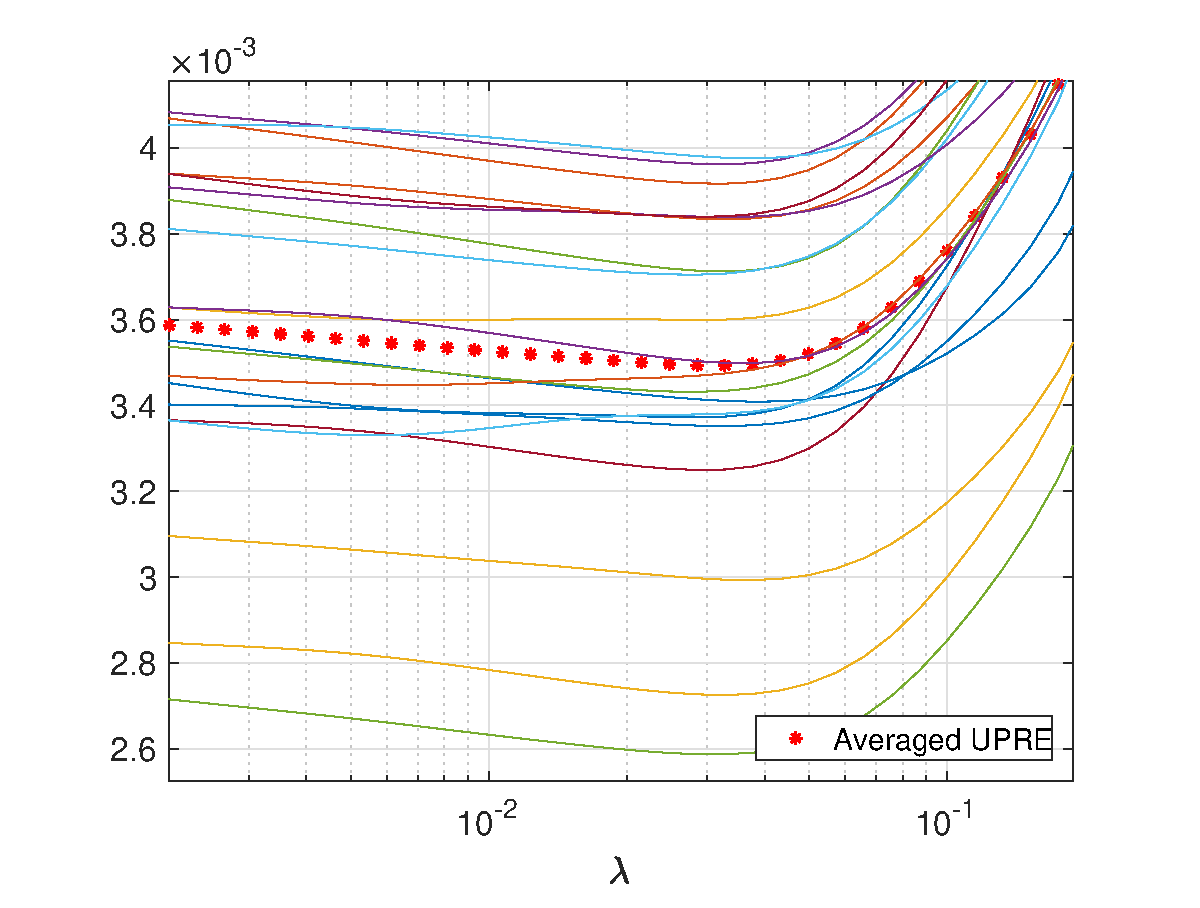
\includegraphics[width=\textwidth]{Figures/UPRE_AvgPlot1D_F1_S15_W100_R20.eps}
        \caption{}
        \label{fig:UPREfunctions}
    \end{subfigure}
    \begin{subfigure}[b]{0.45\textwidth}
        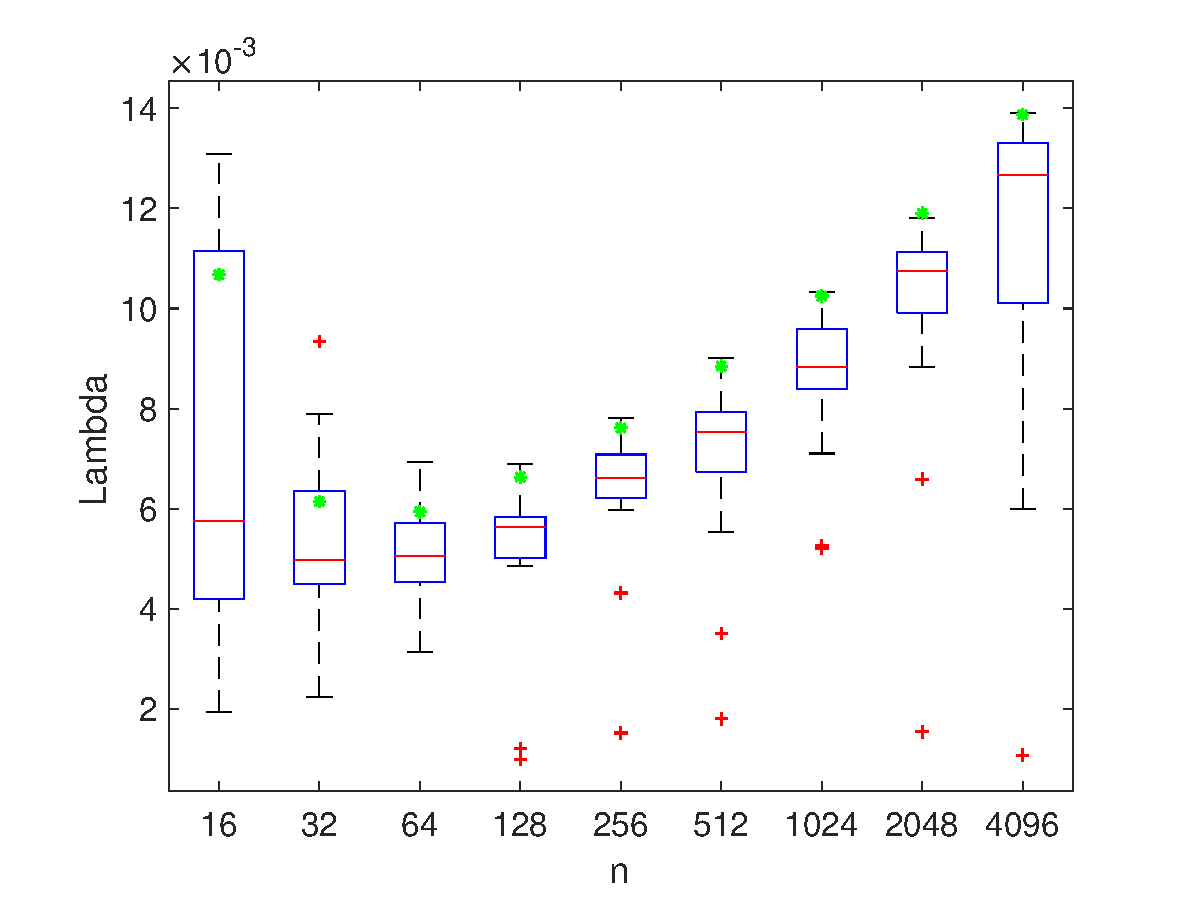
\includegraphics[width=\textwidth]{Figures/UPRE_LamPlot1D_F1_S15_W100_R20.eps}
        \caption{}
        \label{fig:UPRElambdas}
    \end{subfigure}
    \begin{subfigure}[b]{0.45\textwidth}
        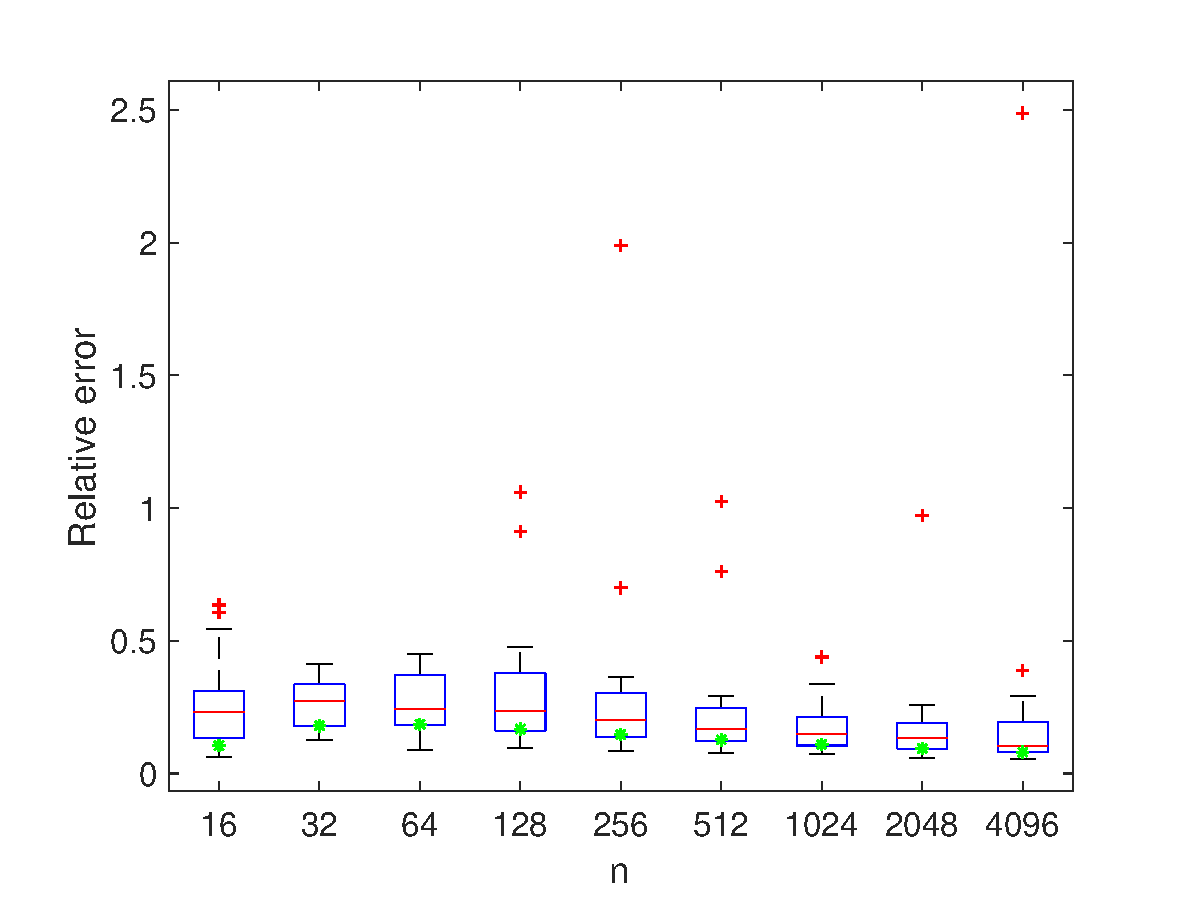
\includegraphics[width=\textwidth]{Figures/UPRE_ErrPlot1D_F1_S15_W100_R20.eps}
        \caption{}
        \label{fig:UPREerrors}
    \end{subfigure}
    \caption{Three plots showing the averaged UPRE results for the first test function with an SNR of 15 and  a Gaussian width parameter of 100. Figure \ref{fig:UPREfunctions} shows a zoomed-in portion of the averaged UPRE graph in comparison with graphs pertaining to the 20 noise realizations at a downsampling level of $n = 128$. Figure \ref{fig:UPRElambdas} shows that the resulting regularization parameter is typically greater than the average of the individual regularization parameters. Figure \ref{fig:UPREerrors} shows that the relative error corresponding to the parameter chosen from the average UPRE method is less than the average of the individual relative errors.}
\label{fig:UPREplots}
\end{figure} 

\subsection{The GCV method} \label{The GCV method}
The numerical results of the GCV method are similar to those of the UPRE method. At times the graphs of the GCV functions are shallow and thus difficult to minimize. This is apparent from the parameter outliers in Figure \ref{fig:GCVlambdas} and the corresponding error outliers in Figure \ref{fig:GCVerrors}. The range of the parameters selected at the $n = 16$ is again significant. Some of the parameters at this level were selected so small (quite near to zero) so that the relative errors were excessively large; the largest relative error was approximately 35, and as a result the vertical axis in Figure \ref{fig:GCVerrors} had to be scaled so that errors larger than 2 are simply grouped in a non-scaled region to produce a tractable plot. \par 
In contrast to the UPRE method, the averaged version of the GCV method selected a regularization parameter that was worse than those selected by using individual noise realizations. The consequence of this is that the corresponding relative errors were larger than the mean of the individual relative errors. Thus the averaged GCV method does not appear to be a viable parameter selection approach. \par 
As previously mentioned, for the minimization-based methods UPRE and GCV, the shallowness of some of the curves made finding a meaningful minimum difficult. The approach that might be worth considering is to find the location of maximum curvature, which follows the observations and analysis presented in \cite{HansenOLeary}. \par 
The signed curvature of a function $f$, assuming appropriate differentiablility, is
\begin{equation}
\kappa(x) = \frac{f''(x)}{(1+(f'(x))^2)^{3/2}}.
\label{Eq:Curvature}
\end{equation}
Including the sign of the curvature is useful since a location of maximum curvature could be associated with local maximum instead of a minimum. A numerical approximation to \eqref{Eq:Curvature} can be readily obtained by discretizing $f$ on the domain of interest and using the finite difference approximations
\[f'(x) \approx \frac{x_{j+1} - x_{j}}{\Delta{x}} \text{ and } f''(x) \approx \frac{x_{j-1} - 2x_j + x_{j+1}}{(\Delta{x})^2}\]
for approximations of the derivatives. In MATLAB, the built-in function \texttt{diff} can be used to generate the derivative approximations. \par 
Once a discretization of curvature is obtained, the location of maximum curvature is determined and this location is taken to be the regularization parameter from the UPRE and GCV methods. While the approach of maximizing curvature is not the same as finding a minimum a function itself, this approach could avoid the numerical challenges of minimizing the shallow UPRE and GCV functions. 

\begin{figure}
	\centering
	\begin{subfigure}[b]{0.45\textwidth}
        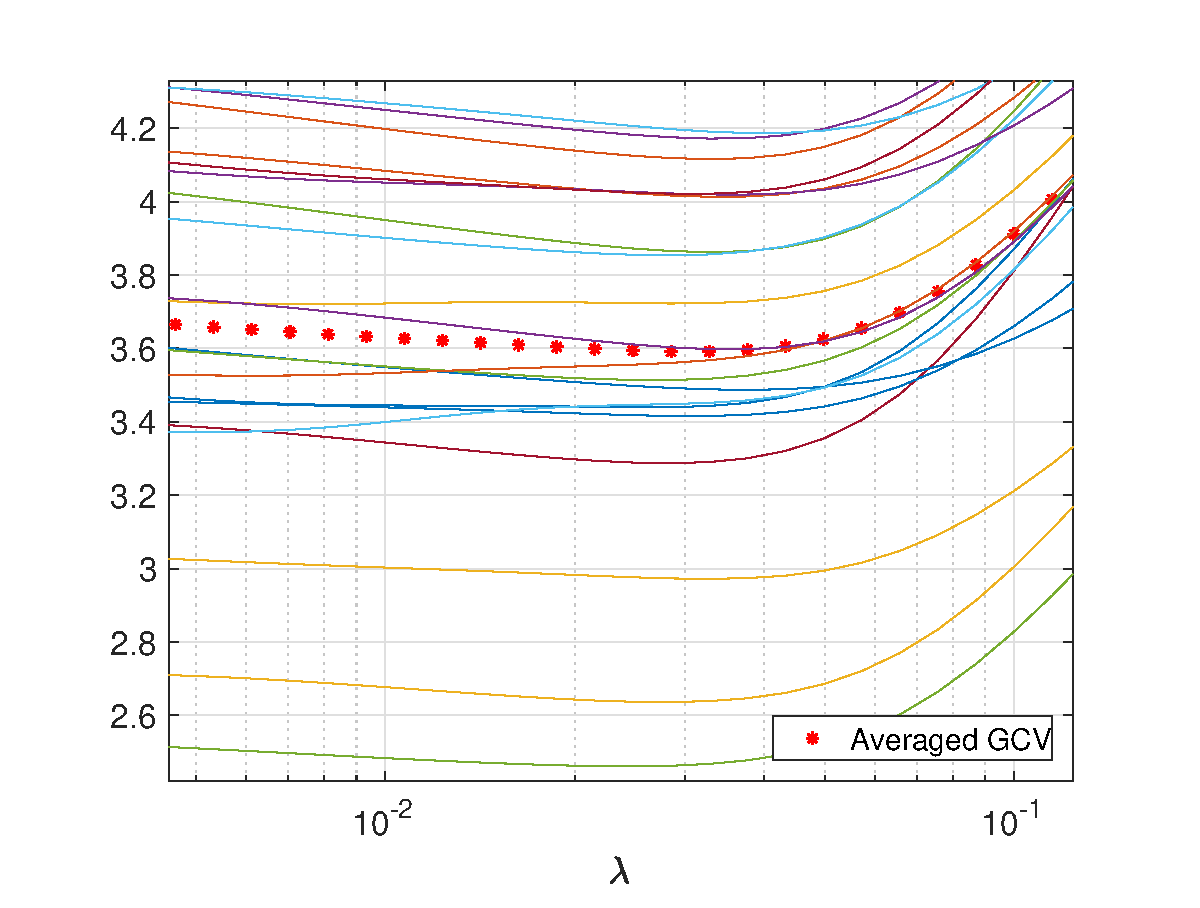
\includegraphics[width=\textwidth]{Figures/GCV_AvgPlot1D_F1_S15_W100_R20.eps}
        \caption{}
        \label{fig:GCVfunctions}
    \end{subfigure}
    \begin{subfigure}[b]{0.45\textwidth}
        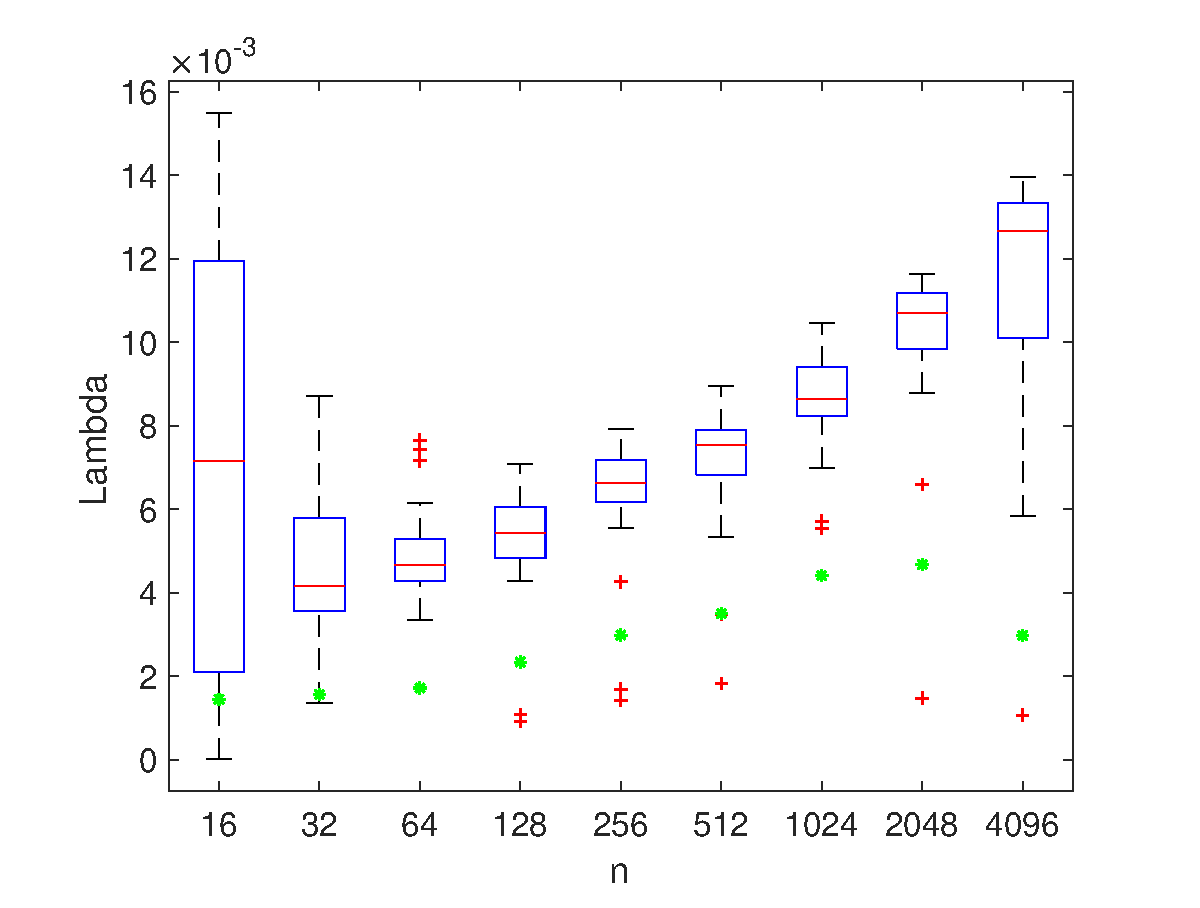
\includegraphics[width=\textwidth]{Figures/GCV_LamPlot1D_F1_S15_W100_R20.eps}
        \caption{}
        \label{fig:GCVlambdas}
    \end{subfigure}
    \begin{subfigure}[b]{0.45\textwidth}
        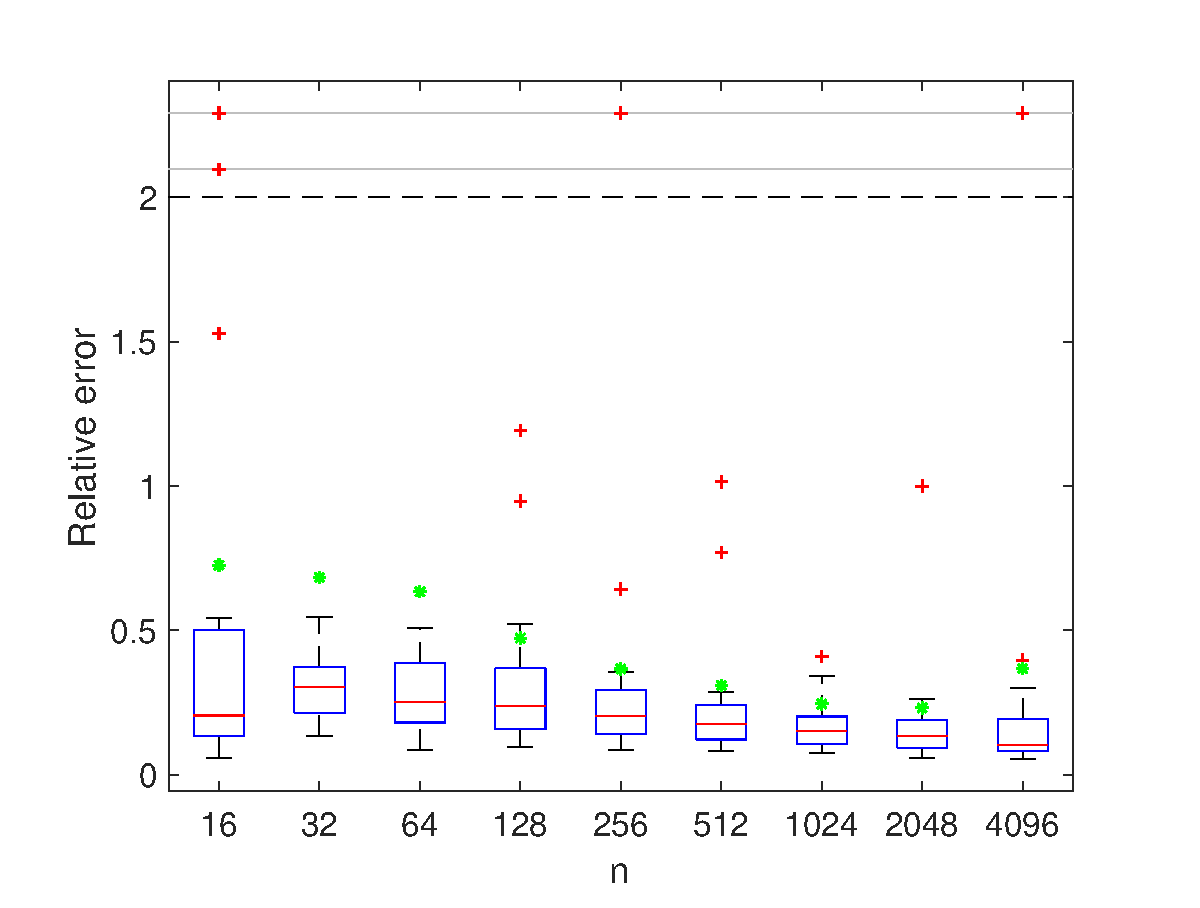
\includegraphics[width=\textwidth]{Figures/GCV_ErrPlot1D_F1_S15_W100_R20.eps}
        \caption{}
        \label{fig:GCVerrors}
    \end{subfigure}
    \caption{Three plots showing the averaged GCV results for the first test function with an SNR of 15 and a Gaussian width parameter of 100. Figure \ref{fig:GCVfunctions} shows a zoomed-in portion of the averaged GCV graph in comparison with graphs pertaining to the 20 noise realizations at a downsampling level of $n = 128$. Figure \ref{fig:GCVlambdas} shows that the resulting regularization parameter is typically less than the average of the individual regularization parameters. Figure \ref{fig:GCVerrors} shows that the relative error corresponding to the parameter chosen from the average GCV method is greater than the average of the individual relative errors.}
\label{fig:GCVplots}
\end{figure}

\subsection{The MDP method} \label{The MDP method}

\begin{figure}
\centering
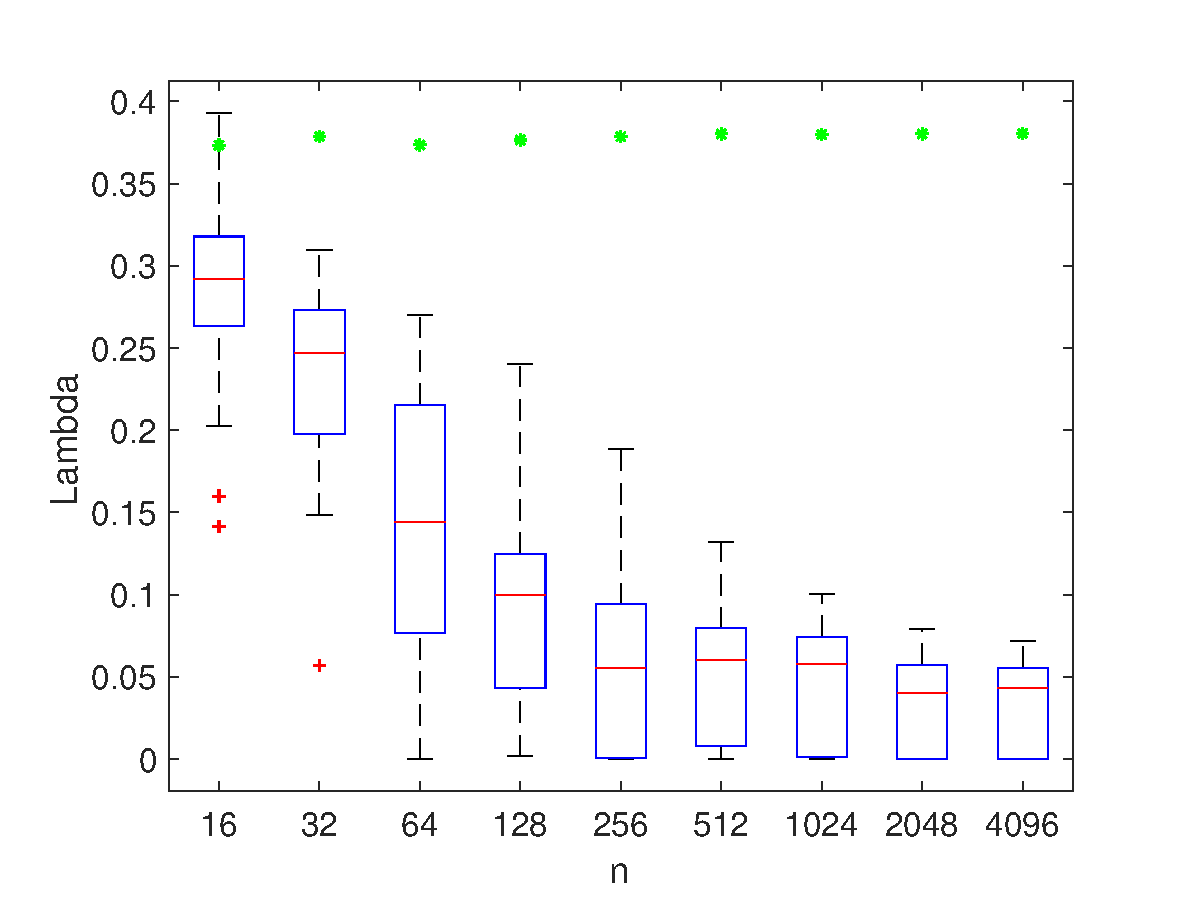
\includegraphics[width=\textwidth]{Figures/MDP_LamPlot1D_F1_S15_W100_R20.eps}
\caption{The parameter selected by the average MDP method appear to be constant, and outside of the range of the parameters found by using the individual noise realizations. This contradicts the lemma in Section \ref{The MDP method}; more investigation is needed.}
\label{fig:MDPlambdas}
\end{figure}

\bibliographystyle{siam}
\bibliography{Parameter-Estimation}

\end{document}
